\documentclass{article}
\usepackage[margin=2.5cm, includefoot, footskip=30pt]{geometry}

\setlength{\parindent}{0em}
\setlength{\parskip}{1em}
\renewcommand{\baselinestretch}{1}

%%%%Packages%%%%
\usepackage{amsmath}
\usepackage{booktabs}
\usepackage{graphics}
\usepackage{multicol}
\usepackage[ruled,vlined]{algorithm2e}
\usepackage{setspace}
\usepackage{graphicx}
\usepackage{subcaption}
\usepackage{hyperref}
\usepackage{color,colortbl}
\usepackage{array}
\usepackage{booktabs}
\usepackage{tabularx}
\usepackage{wrapfig, blindtext}
\usepackage[table]{xcolor}
%%%%%%%%%%%%%%%%%

\definecolor{Gray}{gray}{0.92}
\usepackage[first=0,last=9]{lcg}
\newcommand{\ra}{\rand0.\arabic{rand}}

\newcommand{\uniquenumberofseeds}{11400}
\newcommand{\numberofalltournaments}{45606}
\newcommand{\numberofstrategies}{195}

\setlength{\tabcolsep}{3pt}

\title{A meta analysis of tournaments and an evaluation of performance in the
Iterated Prisoner's Dilemma.}
\author{Nikoleta E. Glynatsi, Vincent A. Knight}
\date{}

\begin{document}

\maketitle

\begin{abstract}
The Iterated Prisoner's Dilemma has been used for decades as a model of
behavioural interactions. From the celebrated performance of Tit for Tat, to the
introduction of the zero-determinant strategies, to the use of sophisticated
structures such as neural networks, the literature has been exploring the
performance of strategies in the game for years. The results of the literature,
however, have been relying on the performance of specific strategies in a finite
number of tournaments. This manuscript evaluates
\numberofstrategies strategies' effectiveness in more than 40000 tournaments.
The top ranked strategies are presented, and moreover, the impact of features on
their success are analysed using machine learning techniques. The analysis
determines that the cooperation ratio of a
strategy in a given tournament compared to the mean and median cooperator is the
most important feature. The conclusions are distinct for different types of
tournaments. For instance a strategy with a theory of mind would aim to be the mean/median
cooperator in standard tournaments, whereas in tournaments with probabilistic
ending it would aim to cooperate 10\% of the times the median cooperator did.
\end{abstract}

\section{Background}

The Iterated Prisoner's Dilemma (IPD) is a repeated two player game that models
behavioural interactions, and more specifically, interactions where
self-interest clashes with collective interest. At each turn of the game both
players, simultaneously and independently, decide between cooperation (C) and
defection (D) whilst having memory of their prior interactions. The payoffs for each
player, at each turn, is influenced by their own choice and the choice of the
other player. The payoffs of the game are generally defined by:

\[\begin{pmatrix}
R & S \\
T & P
\end{pmatrix}\]

where \(T > R > P > S\) and \(2R > T + S\). The most common values used in
the literature~\cite{Axelrod1981} are $R=3, P=1, T=5, S=0$. These values are also
used in this work.

Conceptualising strategies and understanding the best way of playing the game
has been of interest to the scientific community since the formulation of the
game in 1950~\cite{Flood1958}. Following the computer tournaments of Axelrod in the
1980's~\cite{Axelrod1980a, Axelrod1980b}, a strategy's performance in a round
robin computer tournament became a common evaluation technique for newly designed
strategies. Today more than 200 strategies exist in the literature and several
tournaments, following on from Axelrod's, have been undertaken~\cite{Bendor1991,
Harper2017, Kendall2007, Stephens2002, Stewart2012}.

In the 80's, Axelrod performed two computer tournaments~\cite{Axelrod1980a,
Axelrod1980b}. The contestants were strategies submitted in the form of computer
code. They competed against all other entries, a copy of themselves and a random
strategy. The winner was decided on the average score a strategy achieved. The
winner of both tournaments was the simple strategy Tit For Tat which cooperated
on the first turn and then simply copied the previous action of it's opponent.
Due to the strategy's strong performance in both tournaments, and moreover in a
series of evolutionary experiments~\cite{Axelrod1981}, Tit For Tat was thought
to be the most robust basic strategy in the IPD.

However, further research proved that the strategy had weaknesses, and more
specifically, it was shown that the strategy suffered in environments with
noise~\cite{Bendor1991, Donninger1986, Molander1985, Hammerstein1984}. This was
mainly due to the strategy's lack of generosity and contrition. The strategy was
quick to punish a defection, and in a noisy environment it could lead to a
repeated cycle of defections and cooperations. Some new strategies, more
robust in tournaments with noise, were soon introduced and became the new
protagonists of the game. These include Nice and Forgiving~\cite{Bendor1991},
Pavlov~\cite{Nowak1993} and Generous Tit For Tat~\cite{Nowak1992}.

In 2004, a $20^{\text{th}}$ Anniversary Iterated Prisoner Dilemma Tournament
took place with 233 entries. This time the winning strategy was not designed on
a reciprocity based approach but on a mechanism of
teams~\cite{J.P.Delahaye1993Lp, J.P.Delahaye1995LIeP, A.Rogers2007Ctpw}. A team
from Southampton University took advantage of the fact that a participant was
allowed to submit multiple strategies. They submitted a total of 60 strategies
that could recognise each other and colluded to increase one members score.
This resulted with three of the strategies to be ranked in the top spots. The
performance of the Southampton University team received mixed attention, though
they had won the tournament as stated in~\cite{us_blog} "technically this
strategy violates the spirit of the Prisoner's Dilemma, which assumes that the
two prisoners cannot communicate with one another".

Another set of IPD strategies that have received a lot of attention
are the zero-determinant strategies (ZDs)~\cite{Press2012}. By
forcing a linear relationship between the payoffs ZDs can ensure that they will
never receive less than their opponents. The
American Mathematical Society's news section stated that ``the world of game
theory is currently on fire''.
ZDs are indeed a set of mathematically unique strategies
and robust in pairwise interactions, however, their simplicity and extortionate
behaviour have been tested. In~\cite{Harper2017} a tournament containing over
200 strategies, including ZDs, was ran and none of them
ranked in top spots. Instead, the top ranked strategies were a set of
trained strategies based on lookup tables~\cite{Axelrod1987}, hidden markov
models~\cite{Harper2017} and finite state automata~\cite{Miller1996}.

Though only a select pieces of work have been discussed, the IPD literature is
rich, and new strategies and competitions are being published every year~\cite{Glynatsi2019}. The
question, however, still remains the same: what is the best way to play the
game? Compared to other works, whereas a few selected strategies are evaluated
on a small number of tournaments, this manuscript evaluates the performance of \numberofstrategies
strategies in \numberofalltournaments tournaments. These tournaments do not
consist of just standard round robin tournaments, but also tournaments with noise
and tournaments with a probabilistic ending. The later part of the paper, evaluates
the impact of features on the performance of the strategies using modern
machine learning techniques. These features include measures regarding a
strategy's behaviour and measures regarding the tournaments. The data set used
in this work has been made publicly available~\cite{data} and can be used
for further analysis and insights.

The different tournament types as well as the data collection, which is made
possible due to an open source package called Axelrod-Python,
are covered in Section~\ref{section:data_collection}.
Section~\ref{section:top_performances}, focuses on the best performing
strategies for each type of tournament and overall.
Section~\ref{section:evaluation_of_performance}, explores the traits which
contribute to good performance, and finally the results are summarised in
Section~\ref{section:conclusion}. This manuscripts uses several parameters.
These are introduced in the following sections, however, the full set of
parameters and their definitions are given in Appendix~\ref{app:parameters}.
A list of all strategies including citations of their origins is given in
Appendix~\ref{app:list_of_players}.

\section{Data collection}\label{section:data_collection}

For the purposes of this manuscript a data set containing results of IPD
tournaments has been generated and is available at~\cite{data}. This was done using the
open source package Axelrod-Python library~\cite{axelrodproject} (APL), and more specifically,
version 3.0.0. APL allows for different types of IPD computer
tournaments to be simulated whilst containing a list of over 180 strategies.
Most of these are strategies described in the literature with a few exceptions
being strategies that have been contributed specifically to the package. This
paper make use of \numberofstrategies strategies implemented in version 3.0.0. A
list of the strategies is given in the Appendix~\ref{app:list_of_players}.
Though APL features several tournament types, this work considers
standard, noisy, probabilistic ending and noisy probabilistic ending
tournaments.

\textbf{Standard tournaments}, are tournaments similar to that of Axelrod's
in~\cite{Axelrod1980a}. There are \(N\) strategies which all play an iterated
game of \(n\) number of turns against each other. Note that self interactions
are not included. Similarly, \textbf{noisy
tournaments} have \(N\) strategies and \(n\) number of turns, but at each turn
there is a probability \(p_n\) that a player's action will be flipped.
\textbf{Probabilistic ending tournaments}, are of size \(N\) and after each turn
a match between strategies ends with a given probability \(p_e\). Finally,
\textbf{noisy probabilistic ending} tournaments have both a noise probability
\(p_n\) and an ending probability \(p_e\). For smoothing the simulated results a
tournament is repeated for \(k\) number of times. This was allowed to vary 
in order to evaluate the effect of smoothing. The winner of each tournament
is based on the average score a strategy achieved and not by the number of wins.

The process of collecting tournament results implemented in this manuscript is described by
Algorithm~\ref{algorithm:data_generation}. For each trial a random size \(N\) is
selected, and from the \numberofstrategies strategies a random list of \(N\) strategies is
chosen. For the given list of strategies a standard, a noisy, a probabilistic
ending and a noisy probabilistic ending tournament are performed and repeated
\(k\) times. The parameters for the tournaments, as well as the number of
repetitions, are selected once for each trial. The parameters and their
respective minimum and maximum values are given by
Table~\ref{table:parameters_values}.

\begin{table}[!htbp]
    \begin{center}
        \resizebox{.6\textwidth}{!}{
        \begin{tabular}{lcccc}
    \toprule
    parameter & parameter explanation &   min value & max value \\
    \midrule
    $N$ & number of strategies  & 3 & 195 \\
    $k$ & number of repetitions  & 10 & 100 \\
    $n$ & number of turns      & 1 & 200 \\
    $p_n$ & probability of flipping action at each turn  & 0 & 1   \\
    $p_e$ & probability of match ending in the next turn & 0 & 1   \\
    \bottomrule
        \end{tabular}}
    \end{center}
    \caption{Data collection; parameters' values}
    \label{table:parameters_values}
\end{table}

The source code for the data collection, as well as the source code for
the analysis, which will be discussed in the following sections, have been written
following best practices~\cite{Aberdour2007, Benureau2018}. It has been packaged
and is available here. %TODO archive code

\begin{algorithm}[!htbp]
    \setstretch{1.35}
    \ForEach{\text{seed} $\in [0, 11420]$}{
        $N \gets \text{randomly select integer}\in [N_{min}, N_{max}]$\;
        $\text{players} \gets  \text{randomly select $N$ players}$\;
        $k \gets  \text{randomly select integer}\in [k_{min}, k_{max}]$\;
        $n \gets  \text{randomly select integer}\in [n_{min}, n_{max}]$\;
        $p_n \gets  \text{randomly select float}\in [p_{n\, min}, p_{n\, max}]$\;
        $p_e \gets   \text{randomly select float}\in [p_{e\, min}, p_{e\, max}]$\;
        \vspace{0.4cm}
        $\text{result standard}$ $\gets$ Axelrod.tournament$(\text{players}, n, k)$\;
        $\text{result noisy}$ $\gets$ Axelrod.tournament$(\text{players}, n, p_n, k)$\;
        $\text{result probabilistic ending}$ $\gets$ Axelrod.tournament$(\text{players}, p_e, k)$\;
        $\text{result noisy probabilistic ending}$ $\gets$ Axelrod.tournament$(\text{players}, p_n, p_e, k)$\;

    }
    \KwRet{result standard, result noisy, result probabilistic ending,
    result noisy probabilistic ending}\;
    \caption{Data collection Algorithm}
    \label{algorithm:data_generation}
\end{algorithm}

A total of \uniquenumberofseeds trials of Algorithm~\ref{algorithm:data_generation} have been
run. For each trial the results for 4 different tournaments were collected,
thus a total of \numberofalltournaments $(\uniquenumberofseeds \times 4)$ tournament results have been
retrieved. Each tournament outputs a result summary in the form of
Table~\ref{table:output_result}. Each strategy have participated on average in
5154 tournaments of each type. The strategy with the maximum participation in each
tournament type is Inverse Punisher with 5639 entries. The strategy with the
minimum entries is EvolvedLookerUp 1 1 1 which was selected in 4693 trials.

The result summary, Table~\ref{table:output_result}, has \(N\) rows
because each row contains information for each strategy that participated in the
tournament. The information includes the strategy's rank, median score, the rate
with which the strategy cooperated $(C_r)$, its match win count and the
probability that the strategy cooperated in the opening move. Moreover, the
probabilities of a strategy being in any of the four states ($CC, CD, DC, DD$),
and the rate of which the strategy cooperated after each state. A feature that
has been manually included is the \textbf{normalised rank}. The normalised rank,
denoted as $r$, is calculated as a strategy's rank divided by the tournament's
size ($N$). In the next section the performance of these strategies is evaluated
based on their normalised rank.

\newcolumntype{g}{>{\columncolor{Gray}}c}
\begin{table}[!htbp]
    \begin{center}
    \resizebox{\textwidth}{!}{
    \begin{tabular}{ccccccgcgcgcgcg}
    \toprule 
    & & & & & &   \multicolumn{8}{g}{Rates}  \\
    Rank & Name & Median score & Cooperation rating $(C_r)$ & Win & Initial C &
    CC & CD & DC & DD & CC to C & CD to C & DC to C & DD to C \\
    0 &  EvolvedLookerUp2 2 2 & 2.97 & 0.705 & 28.0 & 1.0 & 0.639 & 0.066 & 0.189 &
    0.106 & 0.836 & 0.481 & 0.568 & 0.8 \\
    1 &  Evolved FSM 16 Noise 05 & 2.875 & 0.697 & 21.0 & 1.0 & 0.676 & 
    0.020 & 0.135 & 0.168 & 0.985 & 0.571 & 0.392 & 0.07 \\
    2 & PSO Gambler 1 1 1 & 2.874 & 0.684 &  23.0 &     1.0 &    0.651 &    0.034 &    0.152 &    0.164
    & 1.000 & 0.283 & 0.000 & 0.136 \\
    3 &  PSO Gambler Mem1 &  2.861 &        0.706 &  23.0 &      1.0 &    0.663
    &    0.042 &    0.145 &    0.150 &  1.000 &  0.510 &  0.000 &  0.122 \\
    4 &          Winner12 &  2.835 &        0.682 &  20.0 &      1.0 &
    0.651 &    0.031 &    0.141 &    0.177 &  1.000 &  0.441 &  0.000 &  0.462 \\
    $\dots$ & $\dots$ & $\dots$ & $\dots$ & $\dots$ & $\dots$ & $\dots$ & $\dots$ &
    $\dots$ & $\dots$ & $\dots$ & $\dots$ & $\dots$ & $\dots$ \\
    \bottomrule
    \end{tabular}}
\end{center}
\caption{Output result of a single tournament.}\label{table:output_result}
\end{table}

\section{Top ranked strategies}\label{section:top_performances}

This section evaluates the performance of \numberofstrategies IPD strategies. The performance of
each strategy is evaluated in four tournament types, which were presented in Section
\ref{section:data_collection}, followed by an evaluation of their performance
over all the \numberofalltournaments simulated tournaments of this work.

Each strategy participated in multiple tournaments of the same type (on average 5154).
For example Tit For Tat participated in a total of 5114
tournaments of each type. The strategy's normalised rank distribution in these
is given in Figure~\ref{fig:tit_for_tat_r_distribution}. A value of \(r =
0\) corresponds to a strategy winning the tournament where a value of
\(r = 1\) corresponds to the strategy coming last. Because of the strategies'
multiple entries their performance is evaluated based on the
\textbf{median normalised rank} denoted as \(\bar{r}\).

\begin{figure}[!htbp]
    \centering
    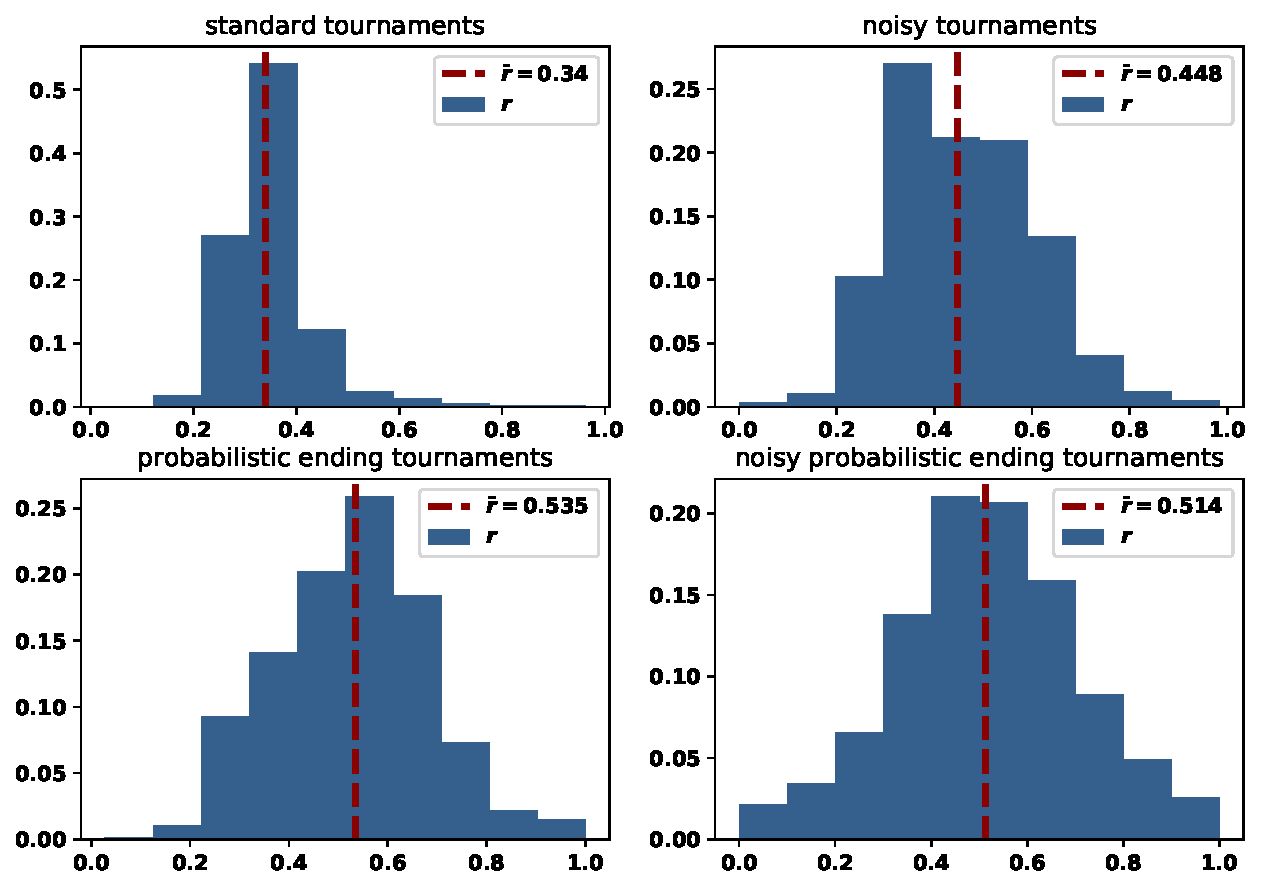
\includegraphics[width=.6\textwidth]{../images/tit_for_tat_r_distributions.pdf}
    \caption{Tit For Tat's $r$ distribution in tournaments. The best performance
    of the strategy has been in standard tournaments where it achieved a $\bar{r}$
    of 0.34.}
    \label{fig:tit_for_tat_r_distribution}
\end{figure}

The top 15 strategies for each tournament type based on \(\bar{r}\) are given in
Table~\ref{table:top_performances}.

\newcolumntype{g}{>{\columncolor{Gray}}l}
\begin{table}[!htbp]
    \begin{center}
    \resizebox{.9\textwidth}{!}{
        \begin{tabular}{lggllggllr}
\toprule
& \multicolumn{2}{g}{Standard} & \multicolumn{2}{c}{Noisy} & \multicolumn{2}{g}{Probabilistic ending} &  \multicolumn{2}{c}{Noisy probabilistic ending} \\
\midrule
& Name & $\bar{r}$ &                 Name & $\bar{r}$ &               Name & $\bar{r}$ &                 Name & $\bar{r}$ \\
\midrule
1 &           Evolved HMM 5 &   0.00667 &               Grumpy &    0.1402 &          Fortress4 &   0.01266 &           Alternator &    0.3037 \\
2 &          Evolved FSM 16 &   0.00995 &                  $e$ &   0.19388 &           Defector &   0.01429 &               $\phi$ &   0.30978 \\
3 &    EvolvedLookerUp2 2 2 &   0.01064 &       Tit For 2 Tats &    0.2069 &  Better and Better &   0.01587 &                  $e$ &    0.3125 \\
4 & Evolved FSM 16 Noise 05 &   0.01667 &         Cycle Hunter &   0.21538 &    Tricky Defector &   0.01875 &                $\pi$ &   0.31686 \\
5 &       PSO Gambler 2 2 2 &   0.02143 &       Risky QLearner &   0.22222 &          Fortress3 &   0.02174 &    Limited Retaliate &   0.35263 \\
6 &             Evolved ANN &   0.02878 &          Retaliate 3 &   0.22887 &     Gradual Killer &   0.02532 &     Anti Tit For Tat &   0.35431 \\
7 &           Evolved ANN 5 &    0.0339 &        Cycler CCCCCD &   0.23507 &         Aggravater &   0.02778 &          Retaliate 3 &   0.35563 \\
8 &       PSO Gambler 1 1 1 &   0.03704 &          Retaliate 2 &   0.23913 &             Raider &   0.03077 &  Limited Retaliate 3 &   0.35563 \\
9 &           Evolved FSM 4 &   0.04891 &      Defector Hunter &   0.24038 &         Cycler DDC &   0.04545 &            Retaliate &   0.35714 \\
10 &        PSO Gambler Mem1 &   0.05036 &            Retaliate &   0.24177 &        Hard Prober &   0.05128 &          Retaliate 2 &   0.35767 \\
11 &                Winner12 &   0.06011 &  Hard Tit For 2 Tats &      0.25 &         SolutionB1 &   0.06024 &  Limited Retaliate 2 &   0.36134 \\
12 &            Fool Me Once &    0.0614 &             ShortMem &   0.25286 &      Meta Minority &   0.06077 &             Hopeless &   0.36842 \\
13 &                     DBS &   0.07143 &  Limited Retaliate 3 &   0.25316 &              Bully &   0.06081 &    Arrogant QLearner &   0.40651 \\
14 &           DoubleCrosser &     0.072 &    Limited Retaliate &   0.25706 &    Fool Me Forever &    0.0708 &    Cautious QLearner &   0.40909 \\
15 &             BackStabber &   0.07519 &                $\pi$ &   0.25801 &             EasyGo &   0.07101 &      Fool Me Forever &   0.41764 \\
\bottomrule
    \end{tabular}
    
    }
\end{center}
\caption{Top performances for each tournament type based on $\bar{r}$.}
\label{table:top_performances}
\end{table}

In standard tournaments 10 out of the 15 top strategies are introduced
in~\cite{Harper2017}. These are strategies based on finite state automata (FSM),
hidden markov models (HMM), artificial neural networks (ANN), lookup tables
(LookerUp) and stochastic lookup tables (Gambler) that have been trained using
reinforcement learning algorithms (evolutionary and particle swarm algorithms).
They have been trained to perform well against the strategies
in APL in a standard tournament, thus their performance in the
specific setting was anticipated. DoubleCrosser, and Fool Me Once, are
strategies not from the literature but from the APL. DoubleCrosser
is a strategy that makes use of the number of turns because it is set to defect on
the last two rounds. The strategy was expected to not perform as well in
tournaments where the number of turns is not specified, but the strategy did not
perform well in tournaments with noise either. Finally, Winner
12~\cite{mathieu2017} and DBS~\cite{Au2006} are both from the the literature.
DBS is strategy specifically designed for noisy environments, however, it ranks
highly only in standard ones.

Figure~\ref{fig:std_results} gives the distributions of $r$ for the top
ranked strategies. The distributions are skewed towards zero and the highest
median, of the top 15 strategies, is at 0.075. This indicates that the top ranked
strategies perform well in any given standard tournament, regardless of the opponents and
the number of turns.

\begin{figure}[!htbp]
    \centering
    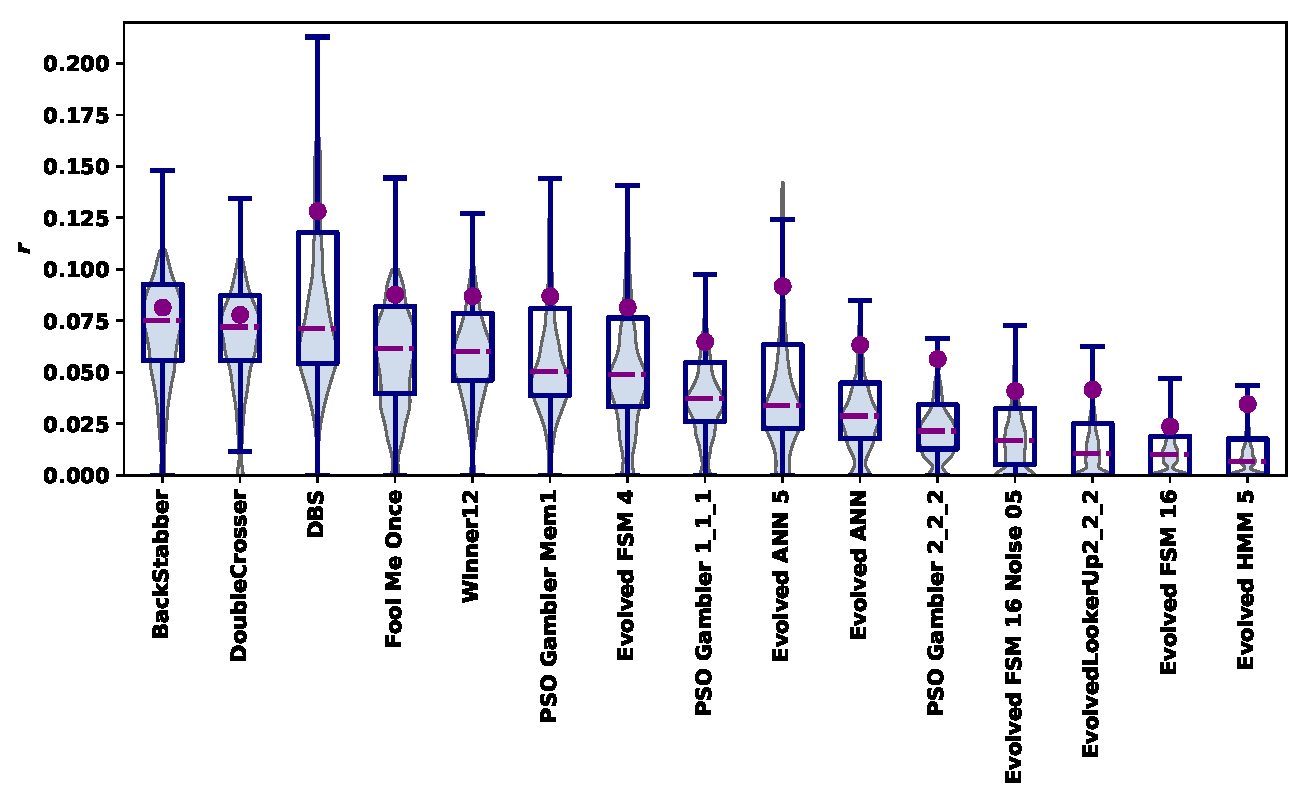
\includegraphics[width=.7\textwidth]{../images/performance_standard.pdf}
    \caption{$r$ distributions of top 15 strategies in standard tournaments.}\label{fig:std_results}
\end{figure}

The top strategies in noisy tournaments are shown in Figure~\ref{fig:noisy_results}. These include deterministic strategies, such
as Tit For 2 Tats~\cite{Axelrod1980b}, Slow Tit For Two Tats~\cite{axelrodproject}, Hard Tit For 2 Tats~\cite{Stewart2012}
and Cycler CCCCCD, and strategies which decide their actions based on the
cooperations to defections ratio, such as ShortMem~\cite{Carvalho2013}, Grumpy
and $e$~\cite{axelrodproject}. Slow Tit For Two Tats is the same strategy as 
Tit For 2 Tats, and at the time of writing this manuscript the
contributors of~\cite{axelrodproject} made a new release where the strategy
has been removed. However, for the purpose of this work the strategy is kept.
The Retaliate and
Limited Retaliate strategies are implemented in APL by the
same contributor. They are strategies designed to defect if the opponent has
tricked them more often than \(x\%\) of the times that they have
done the same. Finally, in $4^{\text{th}}$ and $9^{\text{th}}$ place are Hunter
strategies which try to extort strategies that play cyclically
and defectors.

From Figure~\ref{fig:noisy_results}, it is evident that the normalised rank
distributions in noisy environments are more variant with higher medians
compared to standard tournaments. The distributions are bimodal. This indicates
that although the top ranked strategies mainly performed well, there are several
tournaments that they ranked in the bottom half. To gain a better understanding
of the behaviour in noisy tournaments, the \(r\) distributions for the top 6
of Figure~\ref{fig:noisy_results} strategies over the noise probability \(p_n\),
are given in Figure~\ref{fig:effect_of_noise}.

\begin{figure}[!htbp]
    \centering
    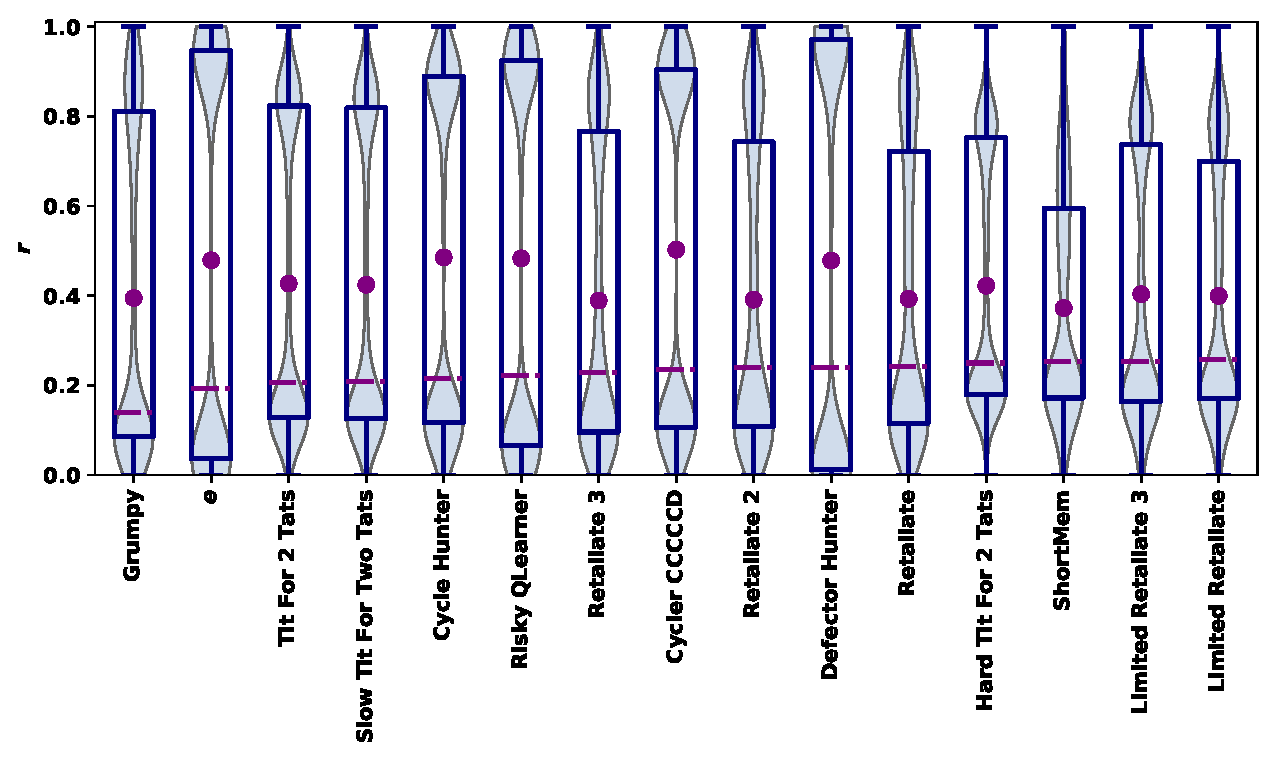
\includegraphics[width=.7\textwidth]{../images/performance_noise.pdf}
    \caption{\(r\) distributions for best performed strategies in noisy tournaments.}
    \label{fig:noisy_results}
\end{figure}

Figure~\ref{fig:effect_of_noise} shows that for \(p_n\) values lower than 0.5
Grumpy, Tit For 2 Tats and Slow Tit For Two Tat perform moderately, and \(e\),
Cycle Hunter and Ricky QLearner perform poorly. At \(p_n=0.5\) all the
distributions become bimodal. This is because with a noise probability of 0.5,
all strategies correspond to a random player. Interestedly, for a \(p_n\) larger
than 0.5 all of the 6 strategies become successful. Note that a value \(p_n=1\)
corresponds to a strategy playing opposite from what it intended to. Thus, it is
demonstrated that the successful strategies is noisy tournaments are sometimes
effective when \(p_n=0.5\) but overall they are very successful whn they are
playing opposite from their original design. If during the data collection a
\(p_n\) strictly less 0.5 was considered then the top ranked strategies would be
different. There are a total of 5661 trials where \(p_n<0.5\) and the top ranked
strategies are given in Table~\ref{table:subset_noise_result}. The median ranks
are lower than before and the top spots are mainly overtaken by Meta strategies
which include NMWE deterministic and NMWE Long Memory. The Meta
strategies~\cite{axelrodproject} create a team of strategies for themselves and
choose to play as a member of their team based on their scores against a given
opponent.

\begin{figure}[!htbp]
    \centering
    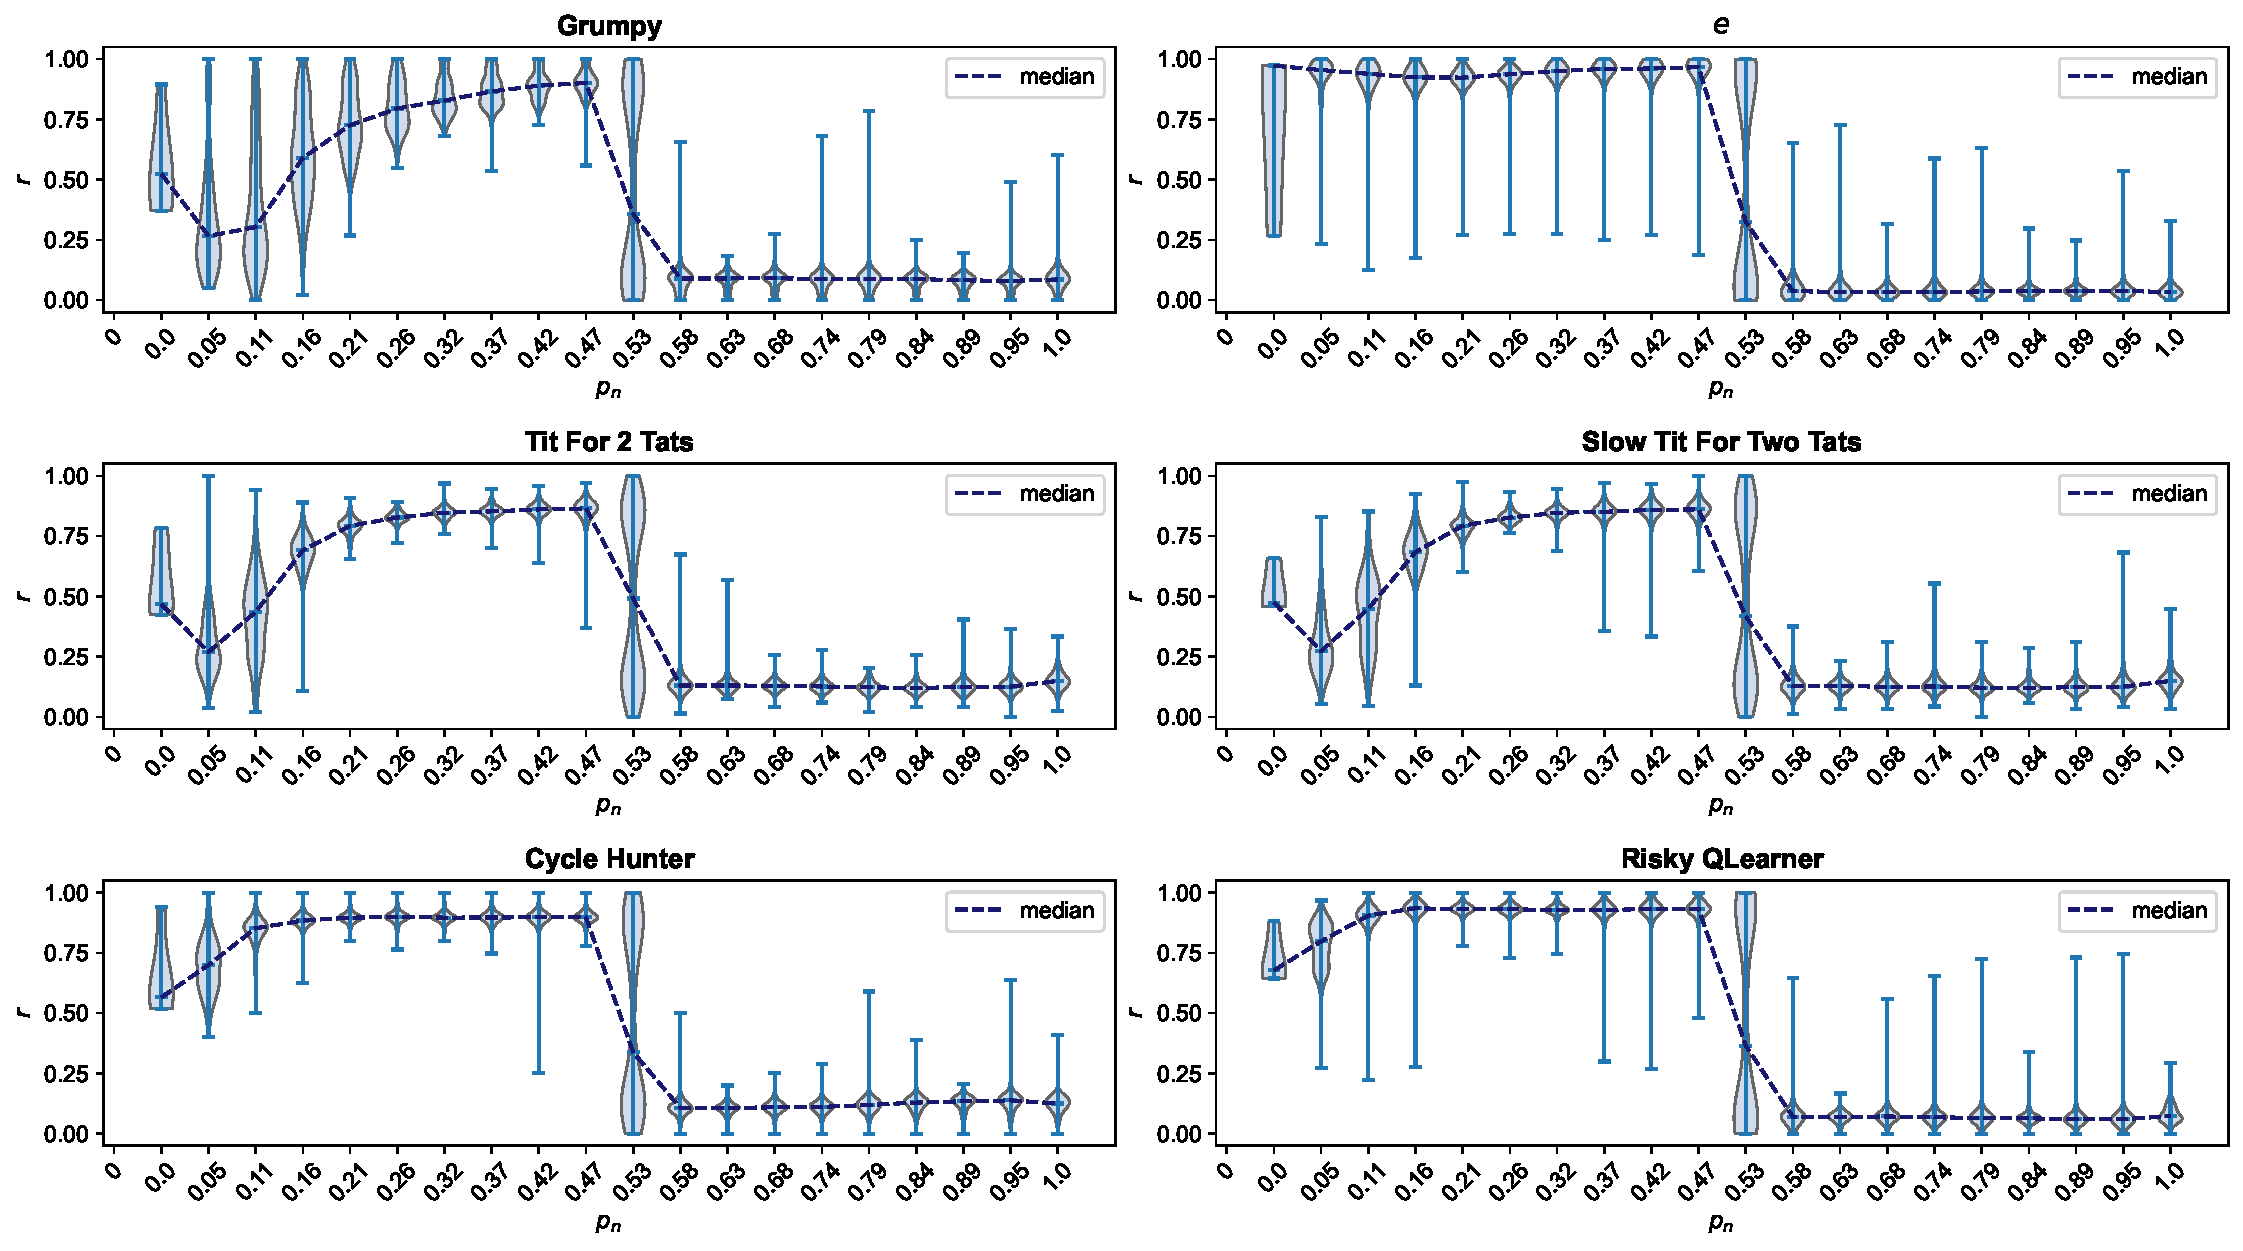
\includegraphics[width=\textwidth]{../images/noise_effect.pdf}
    \caption{\(r\) distributions for top 6 strategies in noisy tournaments over
    the probability of noisy ($p_n$).}
    \label{fig:effect_of_noise}
\end{figure}

\begin{table}[!htbp]
    \centering
    \resizebox{.30\textwidth}{!}{
    \begin{tabular}{lc}
\toprule
Name                      &  $\bar{r}$ \\
\midrule
MEM2                      &    0.06135 \\
Spiteful Tit For Tat      &    0.06344 \\
Nice Meta Winner          &    0.06620 \\
Grudger                   &    0.06667 \\
Meta Winner Long Memory   &    0.07339 \\
Forgiver                  &    0.07362 \\
Fool Me Once              &    0.07362 \\
Meta Winner               &    0.07487 \\
Meta Winner Memory One    &    0.07621 \\
Meta Winner Finite Memory &    0.07692 \\
Meta Winner Deterministic &    0.07792 \\
NMWE Deterministic        &    0.08696 \\
NMWE Long Memory          &    0.08696 \\
CollectiveStrategy        &    0.08696 \\
Defector                  &    0.08889 \\
\bottomrule
\end{tabular}
}
    \caption{Top performances in 5661 noisy tournaments where \(p_n<0.5\).}\label{table:subset_noise_result}
\end{table}

The 15 top ranked strategies in probabilistic ending tournaments include
Fortress 3, Fortress 4 (both introduced in~\cite{Ashlock2006}),
Raider~\cite{Ashlock2014} and Solution B1~\cite{Ashlock2014}, which are
strategies based on finite state automata introduced by Daniel and Wendy
Ashlock. These strategies have been evolved using reinforcement learning, however,
there were trained to maximise their payoffs in tournaments with fixed turns
(150 specifically) and not in probabilistic ending ones. In probabilistic ending
tournaments it appears that the top ranks are mostly occupied by defecting
strategies. These include Better and Better, Gradual Killer, Hard Prober (all
from ~\cite{prison}), Bully (Reverse Tit For Tat)~\cite{Nachbar1992} and
Defector. Thus, it's surprisingly that EasyGo and Fool Me Forever which are
strategies that will defect until their opponent defect, then they will cooperate
until the end, ranked $14^{\text{th}}$ and $15^{\text{th}}$. Upon inspection,
it was found that they are actually the same strategy. This was not known to
the authors at the time of data collection. Figure~\ref{fig:probend_results}
verifies that their performance is the same. Both strategies have repeatedly
ranked highly and there are cases for which they were the winners of the
tournament.

The distributions of the normalised rank in probabilistic ending tournaments,
shown in
Figure~\ref{fig:probend_results}, are less variant than those of noisy
tournaments. The medians of the top 15 strategies are lower than 0.1 and the distributions are skewed
towards 0. Though the large difference between the means and the medians
indicates some outliers, the strategies have overall performed well in the
probabilistic ending tournaments that they participated.

\begin{figure}[h!]
    \centering
    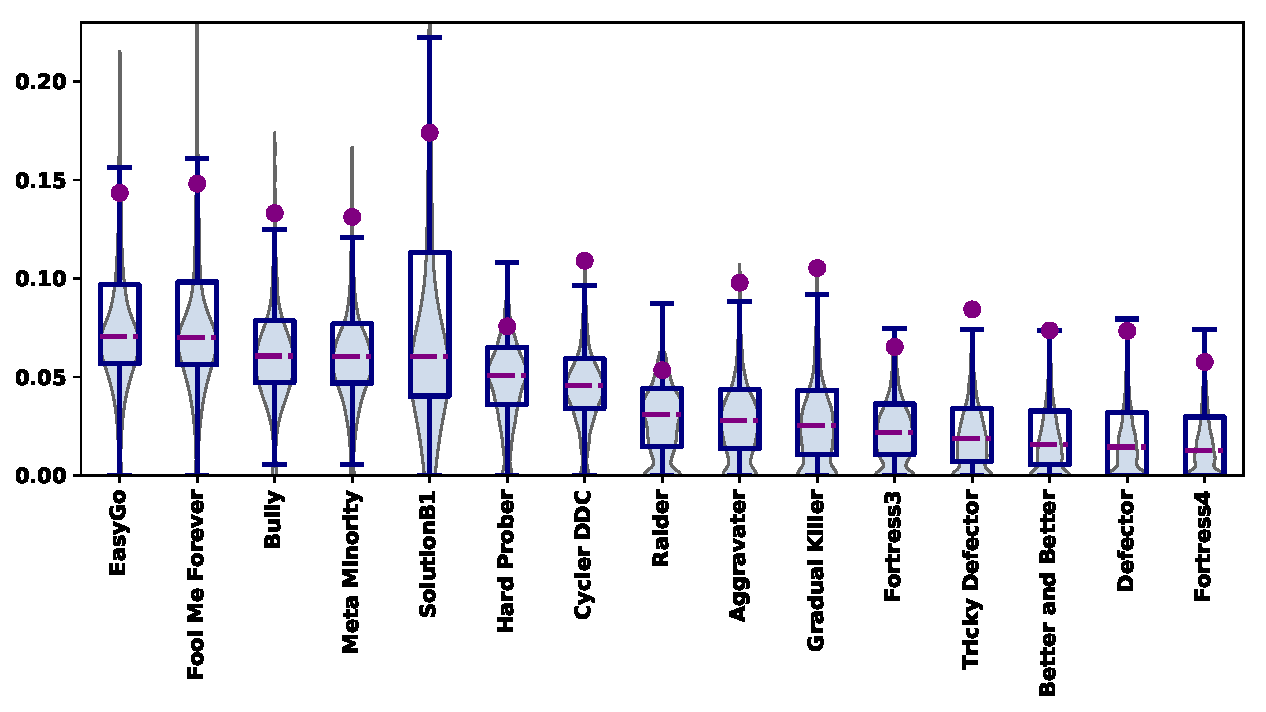
\includegraphics[width=.7\textwidth]{../images/performance_probend.pdf}
    \caption{\(r\) distributions for best performed strategies in probabilistic ending tournaments.}
    \label{fig:probend_results}
\end{figure}

The distributions of \(r\) for the top 6 strategies in probabilistic ending
tournaments over \(p_e\) are given in Figure~\ref{fig:effect_of_probend}.
Figure~\ref{fig:effect_of_probend} shows that the 6 strategies start of with a
high median rank, however, their ranked decreased as the the probability of the
game ending increased and at the point of \(p_e=0.1\) they became the dominant
strategies in their respective tournaments. In essence, what is demonstrated is
that defecting strategies did better when the likelihood of the game ending in
the next turn increased, which is inline with the Folk
Theorem~\cite{Fudenberg2009}. If tournaments where the probability of the game
ending was less than 0.1 were considered then the the top ranked spots are not
dominated by just defecting strategies anymore, as shown in
Table~\ref{table:subset_probend_result}. Instead the effective strategies are
now the Meta strategies, trained strategies, Grudger~\cite{axelrodproject} and
Spiteful Tit for Tat~\cite{prison}.

\begin{figure}[!htbp]
    \centering
    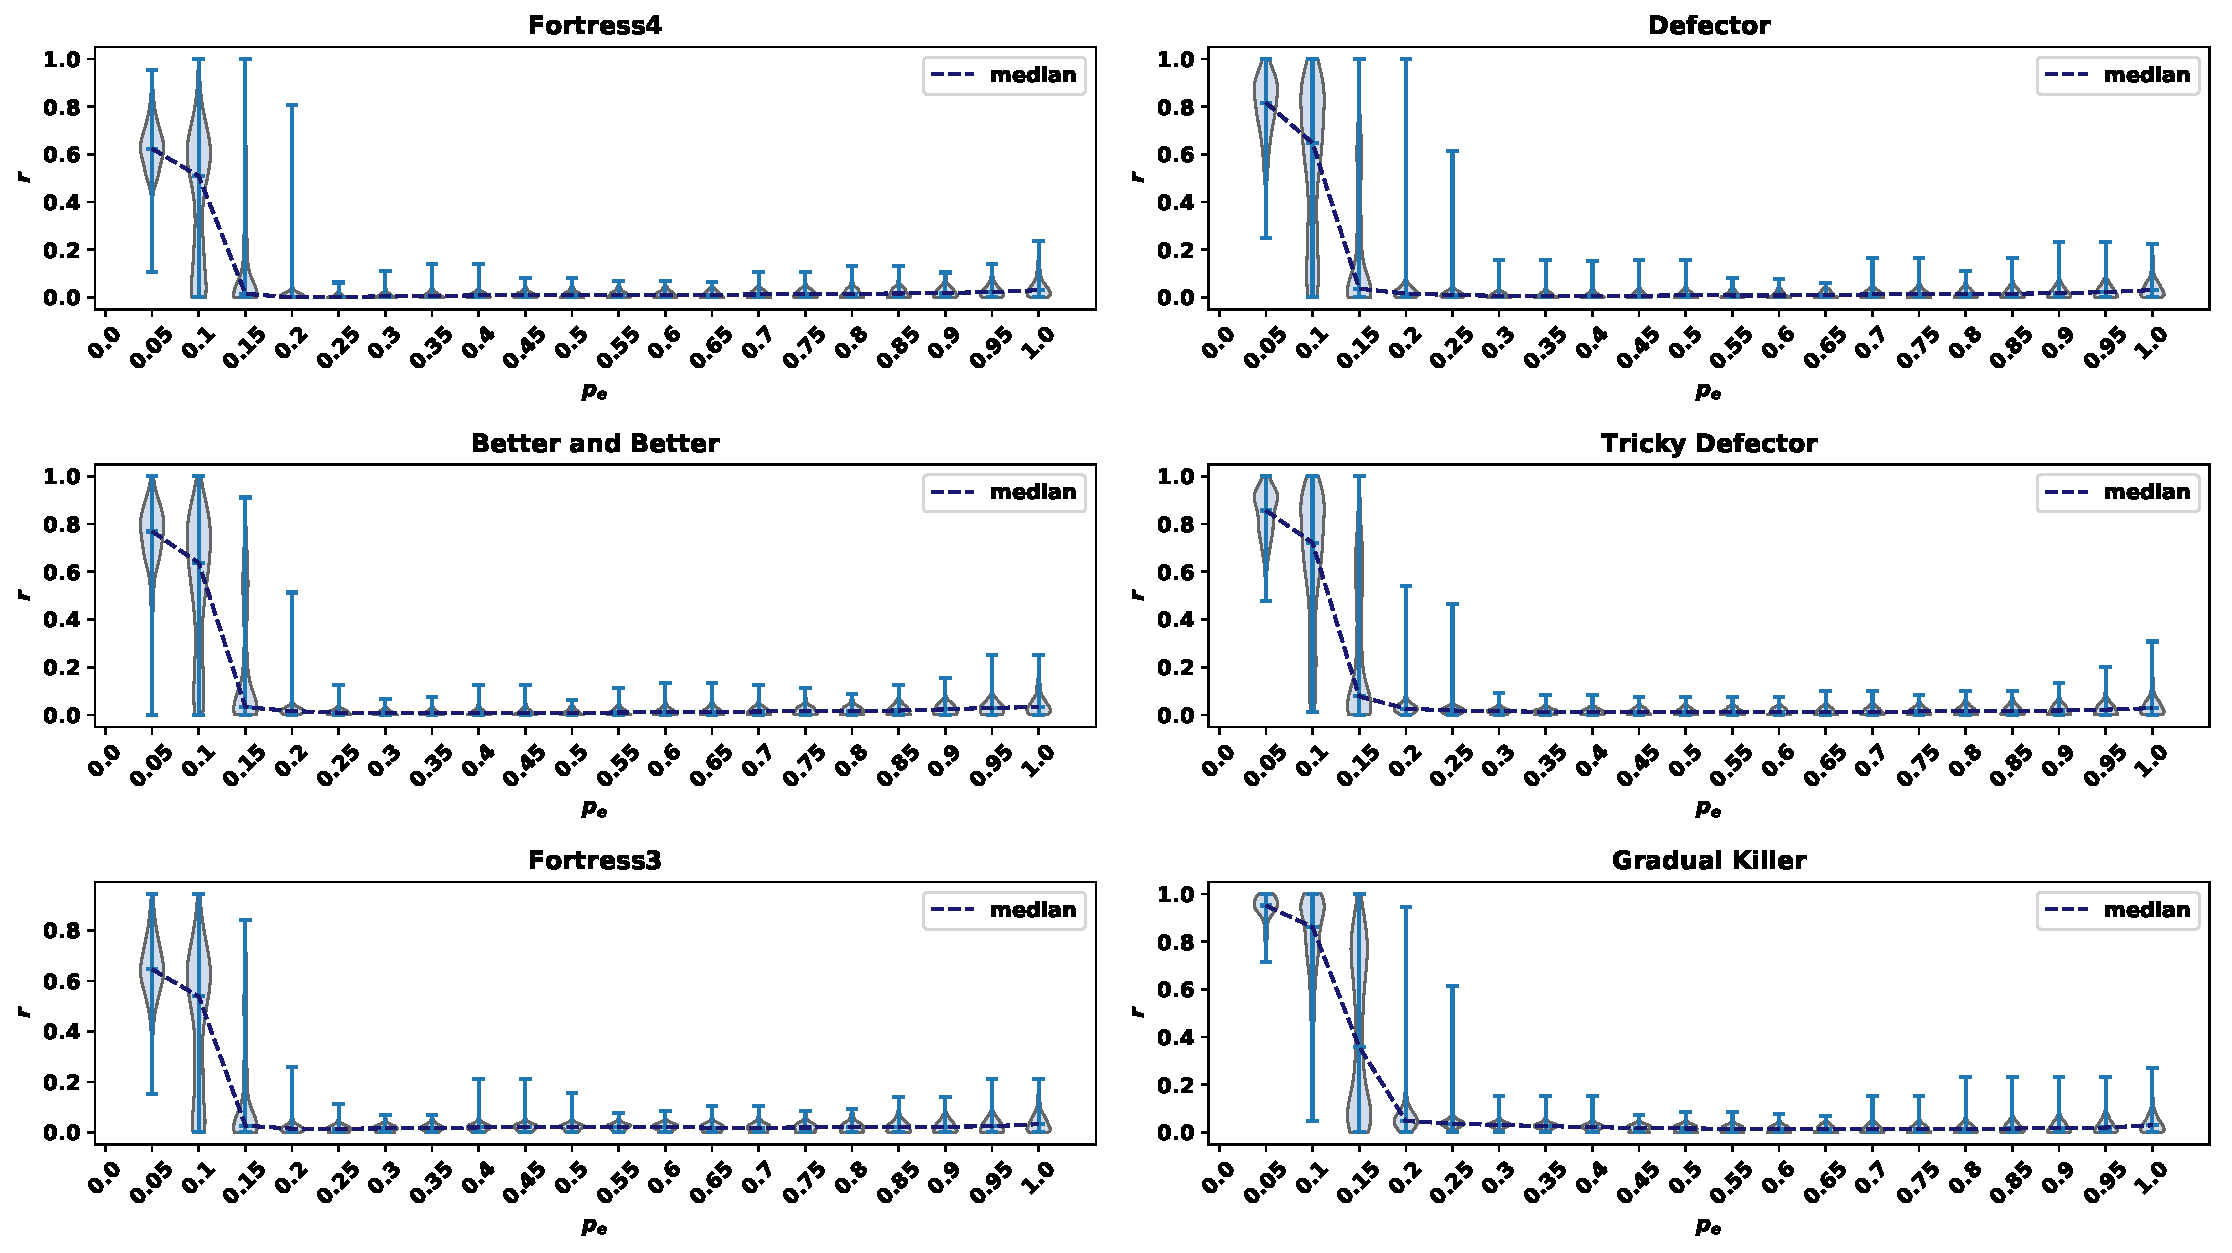
\includegraphics[width=\textwidth]{../images/folk_theorem.pdf}
    \caption{\(r\) distributions for top 6 strategies in probabilistic ending tournaments
    over $p_e$.}
    \label{fig:effect_of_probend}
\end{figure}

\begin{table}[!htbp]
    \centering
    \resizebox{.30\textwidth}{!}{
    \begin{tabular}{lr}
\toprule
Name                      &   $\bar{r}$ \\
\midrule
Evolved FSM 16            &    0.00000 \\
Evolved FSM 16 Noise 05   &    0.01266 \\
MEM2                      &    0.02715 \\
Evolved HMM 5             &    0.04423 \\
EvolvedLookerUp2 2 2      &    0.04870 \\
Spiteful Tit For Tat      &    0.05958 \\
Nice Meta Winner          &    0.06842 \\
NMWE Finite Memory        &    0.06923 \\
Grudger                   &    0.06985 \\
NMWE Deterministic        &    0.07018 \\
NMWE Long Memory          &    0.07407 \\
Nice Meta Winner Ensemble &    0.07595 \\
EvolvedLookerUp1 1 1      &    0.07692 \\
NMWE Memory One           &    0.08000 \\
NMWE Stochastic           &    0.08475 \\
\bottomrule
\end{tabular}
}
    \caption{Top performances in 1139 probabilistic ending tournaments with \(p_e < 0.1\)}
    \label{table:subset_probend_result}
\end{table}

In tournaments with both noise and an unspecified number of turns several of the
top ranked strategies are strategies that were highly ranked in noisy
tournaments. However, strategies from the top ranks in probabilistic ending
tournaments did not rank highly here. Other strategies include $\pi$, $\phi$
which are based on the same approach as $e$. The distributions of \(r\) shown in
Figure~\ref{fig:noisy_probend_results} have the largest median values compared
to the top rank strategies of the other tournament types. A subset of noisy
probabilistic ending tournaments has been considered such that \(p_e < 0.1\) and
\(p_n < 0.5\). The top ranked strategies are given in
Table~\ref{table:subset_probend_noise_result} and it is shown that the Meta
strategies which performed well in noisy tournaments with \(p_n < 0.5\), perform
well once again even the number of turns is not specified. Moreover, several
strategies that did well in probabilistic ending tournaments such as Fortress 3,
Fortress 4, Defector and Better and Better are effective here as well.

\begin{figure}[!htbp]
    \centering
    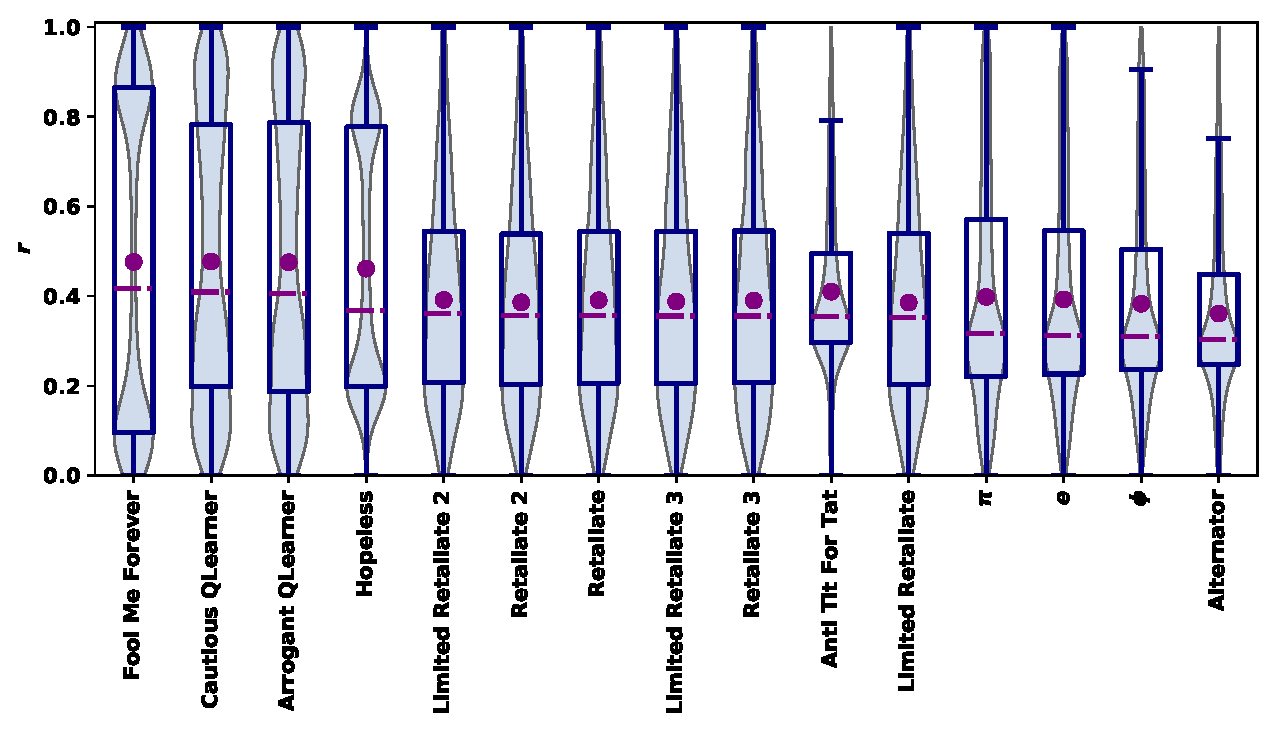
\includegraphics[width=.7\textwidth]{../images/performance_probend_noise.pdf}
    \caption{\(r\) distributions for best performed strategies in noisy
    probabilistic ending tournaments.}
    \label{fig:noisy_probend_results}
\end{figure}

\begin{table}[!htbp]
    \centering
    \resizebox{.30\textwidth}{!}{
    \begin{tabular}{lc}
\toprule
Name                      &    $\bar{r}$\\
\midrule
Defector                  &    0.00552 \\
Better and Better         &    0.01055 \\
Aggravater                &    0.01399 \\
Fortress4                 &    0.02100 \\
Tricky Defector           &    0.03857 \\
Meta Winner Long Memory   &    0.04878 \\
Meta Winner Memory One    &    0.04955 \\
Meta Winner Finite Memory &    0.04972 \\
Meta Winner Stochastic    &    0.05128 \\
Meta Winner Deterministic &    0.05195 \\
Meta Winner               &    0.05333 \\
Meta Winner Ensemble      &    0.05882 \\
Fortress3                 &    0.06956 \\
CollectiveStrategy        &    0.07692 \\
Prober 3                  &    0.08018 \\
\bottomrule
\end{tabular}
}
    \caption{Top performances in 568 probabilistic ending tournaments with \(p_e < 0.1\) and \(p_n < 0.5\).}
    \label{table:subset_probend_noise_result}
\end{table}

Up till now, the performances of the \numberofstrategies strategies have been evaluated for
individual tournament types. The distributions of \(r\) for the tournament types indicate that
for probabilistic ending and standard tournaments successful strategies do exist.
For these settings, the top 15 strategies have frequently ranked in
the top spots with only a few exceptions. Contrarily, it appears that noise
cause variation in the normalised ranks, and the strategies can always guarantee
a spot in the top ranks.

The data set considered in this work, described in
Section~\ref{section:data_collection}, contains a total of \numberofalltournaments
tournament results. For this part of the manuscript the strategies are ranked
based on the median normalised rank they achieved over the entire data set.
The top 15 strategies are given in Table~\ref{table:overall_results}
and their normalised rank distributions are given in Figure~\ref{fig:overall_results}.

\begin{table}[!htbp]
    \centering
    \resizebox{.35\textwidth}{!}{
    \begin{tabular}{lr}
\toprule
{} &  Normalized\_Rank \\
Name                    &                  \\
\midrule
Evolved FSM 16          &            0.018 \\
Evolved HMM 5           &            0.019 \\
Evolved FSM 16 Noise 05 &            0.025 \\
EvolvedLookerUp2\_2\_2    &            0.028 \\
Evolved ANN             &            0.037 \\
PSO Gambler 2\_2\_2       &            0.040 \\
Evolved ANN 5           &            0.046 \\
PSO Gambler 1\_1\_1       &            0.061 \\
Fool Me Once            &            0.067 \\
Evolved FSM 4           &            0.075 \\
DoubleCrosser           &            0.079 \\
Winner12                &            0.081 \\
BackStabber             &            0.082 \\
DBS                     &            0.086 \\
PSO Gambler Mem1        &            0.089 \\
\bottomrule
\end{tabular}
}
    \caption{Top performances over all the tournaments}\label{table:overall_results}
\end{table}

The top ranks include strategies that have been previously mentioned. The
set of Retaliate strategies occupy the top spots followed by BackStabber
and DoubleCrosser. The distributions of the Retaliate strategies have no
statistical difference. Thus, in an IPD tournament where the type is not
specified, playing as any of the Retaliate strategies seems like a good approach.
DoubleCrosser performed well in standard tournaments and the
strategy is just an extension of BackStabber. It should be noted that these
strategies can be characterised as ``cheaters". The source code of the strategies
allows them to known the number of turns in a match (if they are specified).
PSO Gambler and Evolved HMM 5 are
trained strategies introduced in~\cite{Harper2017} and Nice Meta Winner and NMWE
Memory One are strategies based on teams. Grudger is a strategy from Axelrod's
original tournament and Forgetful Fool Me Once is based on the same approach as
Grudger. Overall the top 15 strategies are fundamentally different. Some are cheaters,
some are complex, others are simple deterministic strategies and strategies based
on teams. The results of \numberofalltournaments tournaments used in this work imply the following:
there is not a single type of strategy which can performance well in any IPD interaction.

\begin{figure}[!htbp]
    \centering
    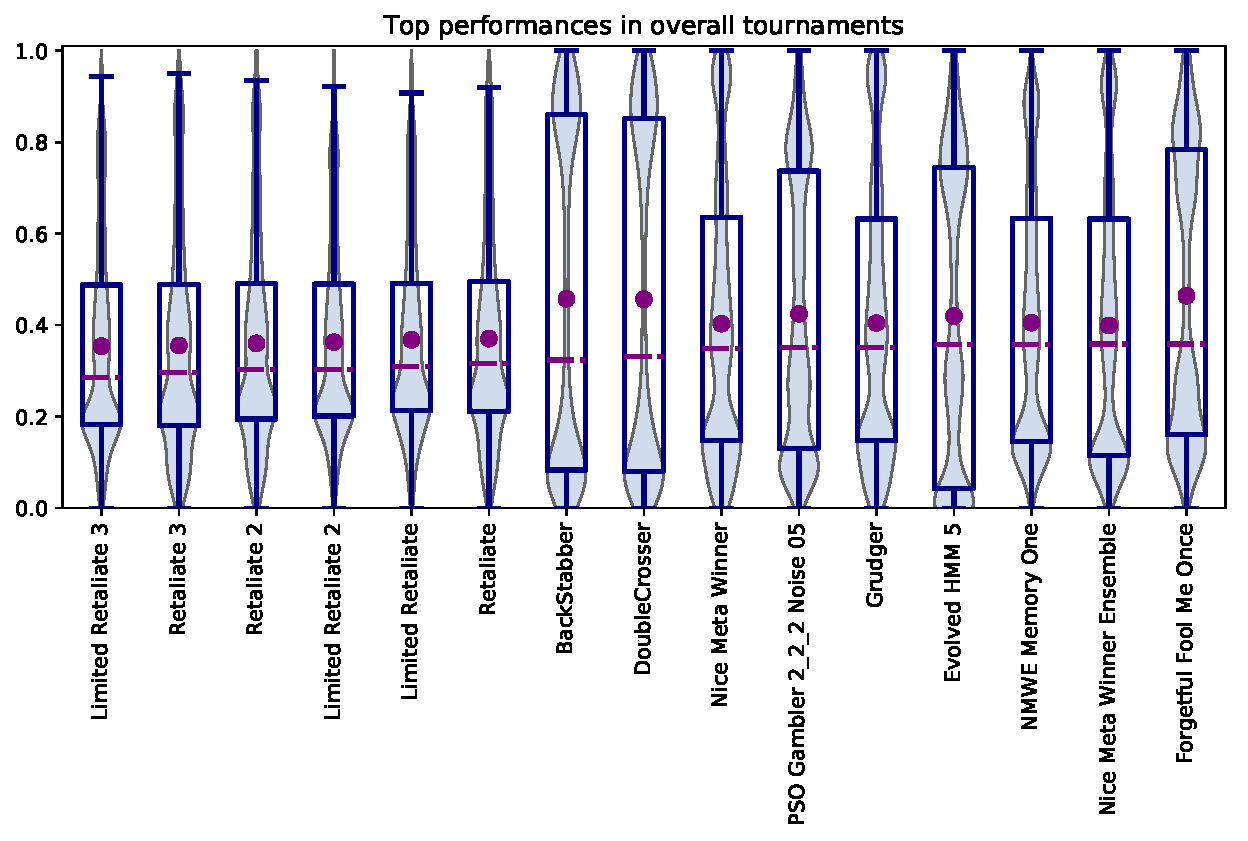
\includegraphics[width=.7\textwidth]{../images/performance_merged.pdf}
    \caption{\(r\) distributions for best performed strategies in the data set~\cite{data}.}
    \label{fig:overall_results}
\end{figure}

This section presented the winning strategies in a series of IPD tournaments. In
standard tournaments the top spots were dominated by complex strategies that had
been trained using reinforcement learning techniques. In noisy environments,
whether the number of turns was fixed or not, the winning strategies were
deterministic strategies designed to defect if the opponent tricked them more
than a current amount of the times that they had tricked their opponent. However,
if a value of noise strictly less than 0.5 was considered, then the successful
strategies were strategies based on teams. In
probabilistic ending tournaments most of the winning strategies were defecting
strategies and trained finite state automata, designed by the same authors.
These strategies only did better when the probability of the game ending after
each turn was increased.
Finally the performance of all \numberofstrategies
strategies over the \numberofalltournaments tournaments in this manuscript was
assessed on \(\bar{r}\). The top ranked strategies were a mixture of behaviours
that did well in standard tournaments and tournaments with noise, as well as a
few strategies based on teams.

The results of this section imply that successful strategies for specific
settings exist for an IPD tournament. The top ranked strategies in both standard
tournaments and tournaments with probabilistic ending, managed to rank in the
top 10\% of the tournament most of the times.
Strategies in noisy
environments demonstrated that no strategy can be consistently
successful, except if the value of noise is constrained to less than a half.
Overall, there has been not a single strategy that has shown to perform well in
more than one setting. The aim of the next section is to understand the features
that made these strategies successful, in each setting separately
but also overall.

\section{Evaluation of performance}\label{section:evaluation_of_performance}

The aim of this section is to explore the features that contribute to a
strategy's successful performance. The features explored are measures regarding a
strategy's behaviour, along with measures regarding the tournaments the
strategies competed in. These are given in Table~\ref{table:manual_features}.

\newcolumntype{g}{>{\columncolor{Gray}}c}
\begin{table}[h]
    \begin{center}
    \resizebox{\textwidth}{!}{
    \begin{tabular}{gcgcgc}
    \toprule
    feature & feature explanation &  source & value type & min value & max value \\
    \midrule
stochastic  &  If a strategy is stochastic & strategy classifier from APL & boolean  & Na &  Na \\
makes use of game &  If a strategy makes used of the game information & strategy classifier from APL & boolean  & Na &  Na \\
makes use of length &  If a strategy makes used of the number of turns & strategy classifier from APL & boolean  & Na &  Na \\
memory usage &  The memory size of a strategy divided by the number of turns & memory size from APL & float & 0 &  1 \\
SSE & A measure of how far a strategy is from ZD behaviour & method described in~\cite{Knight2019} & float & 0 & 1 \\
max cooperating rate $(C_{\text{max}})$  & The biggest cooperating rate in a given tournament  & result summary  & float & 0 & 1\\
min cooperating rate $(C_{\text{min}})$ & The smallest cooperating rate in a given tournament  & result summary  & float & 0 & 1\\
median cooperating rate $(C_{\text{median}})$ & The median cooperating rate in a given tournament  & result summary  & float & 0 & 1\\
mean cooperating rate $(C_{\text{mean}})$ & The mean cooperating rate in a given tournament  & result summary  & float & 0 & 1 \\
$C_r$ / $C_{\text{max}}$ & A strategy's cooperating rate divided by the maximum & result summary  & float & 0 & 1 \\
$C_r$ / $C_{\text{min}}$ & A strategy's cooperating rate divided by the minimum & result summary  & float & 0 & 1 \\
$C_r$ / $C_{\text{median}}$ & A strategy's cooperating rate divided by the median  & result summary  & float & 0 & 1\\
$C_r$ / $C_{\text{mean}}$ & A strategy's cooperating rate divided by the mean & result summary  & float & 0 & 1 \\
$C_r$ & The cooperating ratio of a strategy & result summary  & float & 0 & 1 \\
$CC$ to $C$ rate & The probability a strategy will cooperate after a mutual cooperation & result summary  & float & 0 & 1\\
$CD$ to $C$ rate & The probability a strategy will cooperate after being betrayed by the opponent & result summary  & float & 0 & 1 \\
$DC$ to $C$ rate & The probability a strategy will cooperate after betraying the opponent & result summary  & float & 0 & 1 \\
$DD$ to $C$ rate & The probability a strategy will cooperate after a mutual defection & result summary  & float & 0 & 1 \\
$p_n$ & The probability of a player's action being flip at each interaction & trial summary & float & 0 & 1 \\
$n$ & The number of turns & trial summary & integer & 1 & 200 \\
$p_e$ & The probability of a match ending in the next turn & trial summary & float & 0 & 1 \\
$N$ & The number of strategies in the tournament & trial summary & integer & 3 & 195 \\
$k$ & The number of repetitions of a given tournament & trial summary & integer & 10 & 100 \\
    \bottomrule
        \end{tabular}}
    \end{center}
    \caption{The features which are included in the performance evaluation analysis.}
    \label{table:manual_features}
\end{table}

APL makes use of classifiers to classify strategies according to
various dimensions. These determine whether
a strategy is stochastic or deterministic, whether it makes use of the number of
turns or the game's payoffs. The memory usage feature is calculated as the
memory size of strategy (which is specified in the strategies implementation
in the APL) divide by the number of turns. For example, Evolved
FSM 16 Noise 05 has a memory size of 16 and participated in a tournament where
$n$ was 134. In the given tournament Evolved FSM 16 Noise 05 has a memory usage
of 0.119. For tournaments with a probabilistic ending the number of turns was
not collected, so the memory usage feature is not used for probabilistic ending
tournaments. The SSE is a feature introduced in~\cite{Knight2019} which shows
how close a strategy is to behaving as a ZDs, and subsequently, in an
extortionate way. The method identifies the ZDs closest to a given strategy and
calculates the algebraic distance between them, defined as SSE. A SSE value of 1
indicates no extortionate behaviour at all whereas a value of 0 indicates that a
strategy is behaving a ZDs. The rest of the features considered are the $CC$ to
$C$, $CD$ to $C$, $DC$ to $C$, and $DD$ to $C$ rates as well as cooperating
ratio of a strategy. The minimum, maximum, medium and median cooperating ratios
of each tournament are also included, and finally the number of turns, the
number of strategies, the number of repetitions and the probabilities of noise
and the game ending are also included.

Table~\ref{table:correlations} shows the correlation coefficients between the
features of Table~\ref{table:manual_features} the median score and the median
normalised rank. Note that the correlation for the classifiers is
not included because they are binary variables and they will be evaluated using a
different method. The correlation coefficients for all the features in
Table~\ref{table:manual_features} against themselves have also been calculated and a
graphical representation can be found in the Appendix~\ref{app:correlations}.

\newcolumntype{g}{>{\columncolor{Gray}}c}
\begin{table}[!htbp]
    \begin{center}
    \resizebox{.9\textwidth}{!}{
        \begin{tabular}{lggccggccggg}
    \toprule
    &  \multicolumn{2}{g}{Standard} & \multicolumn{2}{c}{Noisy} & \multicolumn{2}{g}{Probabilistic ending} &  \multicolumn{2}{c}{Noisy probabilistic ending} &  \multicolumn{2}{g}{Overall} \\
\midrule
{} &  $r$ &  median score &  $r$ &  median score &  $r$ &  median score &  $r$ &  median score &  $r$ &  median score\\
\midrule
$CC$ to $C$ rate     & -0.501 &  0.501 &   0.414 &  -0.504 &   0.408 &  -0.323 &   0.260 &   0.022 &  -0.501 &  0.501 \\
$CD$ to $C$ rate     &  0.226 & -0.199 &   0.456 &  -0.330 &   0.320 &  -0.017 &   0.205 &  -0.220 &   0.226 & -0.199 \\
$C_r$                & -0.323 &  0.384 &   0.711 &  -0.678 &   0.714 &  -0.832 &   0.579 &  -0.135 &  -0.323 &  0.384 \\
$C_r$ / $C_{max}$    & -0.323 &  0.381 &   0.616 &  -0.551 &   0.714 &  -0.833 &   0.536 &  -0.116 &  -0.323 &  0.381 \\
$C_r$ / $C_{mean}$   & -0.331 &  0.358 &   0.731 &  -0.740 &   0.721 &  -0.861 &   0.649 &  -0.621 &  -0.331 &  0.358 \\
$C_r$ / $C_{median}$ & -0.331 &  0.353 &   0.652 &  -0.669 &   0.712 &  -0.852 &   0.330 &  -0.466 &  -0.331 &  0.353 \\
$C_r$ / $C_{min}$    &  0.109 & -0.080 &  -0.358 &   0.250 &  -0.134 &   0.150 &  -0.368 &   0.113 &   0.109 & -0.080 \\
$C_{max}$            & -0.000 &  0.049 &   0.000 &   0.023 &  -0.000 &   0.046 &   0.000 &  -0.004 &  -0.000 &  0.049 \\
$C_{mean}$           & -0.000 &  0.229 &  -0.000 &   0.271 &   0.000 &   0.200 &   0.000 &   0.690 &  -0.000 &  0.229 \\
$C_{median}$         &  0.000 &  0.209 &  -0.000 &   0.240 &  -0.000 &   0.187 &  -0.000 &   0.673 &   0.000 &  0.209 \\
$C_{min}$            &  0.000 &  0.084 &   0.000 &  -0.017 &  -0.000 &   0.007 &  -0.000 &   0.041 &   0.000 &  0.084 \\
$DC$ to $C$ rate     &  0.127 & -0.100 &   0.509 &  -0.504 &  -0.018 &   0.033 &   0.341 &  -0.016 &   0.127 & -0.100 \\
$DD$ to $C$ rate     &  0.412 & -0.396 &   0.533 &  -0.436 &  -0.103 &   0.176 &   0.378 &  -0.263 &   0.412 & -0.396 \\
$N$                  &  0.000 & -0.009 &  -0.000 &   0.002 &  -0.000 &   0.003 &  -0.000 &   0.001 &   0.000 & -0.009 \\
$k$                  &  0.000 & -0.002 &  -0.000 &   0.003 &  -0.000 &   0.001 &  -0.000 &  -0.008 &   0.000 & -0.002 \\
$n$                  &  0.000 & -0.125 &  -0.000 &  -0.024 &       - &       - &       - &       - &   0.000 & -0.125 \\
$p_e$                &      - &      - &        - &     - &    0.000 &   0.165 &   0.000 &  -0.058 &  -0.001 &  0.001 \\
$p_n$                &      - &      - &  -0.000 &   0.207 &       - &       - &  -0.000 &  -0.650 &   0.002 & -0.000 \\
Make use of game     & -0.003 & -0.022 &   0.025 &  -0.082 &  -0.053 &  -0.108 &   0.013 &  -0.016 &  -0.003 & -0.022 \\
Make use of length   & -0.158 &  0.124 &   0.005 &  -0.123 &  -0.025 &  -0.090 &   0.014 &  -0.016 &  -0.154 &  0.117 \\
SSE                  &  0.473 & -0.452 &   0.463 &  -0.337 &  -0.156 &   0.223 &   0.305 &  -0.259 &   0.473 & -0.452 \\
memory usage         & -0.082 &  0.095 &  -0.007 &  -0.017 &       - &     - &     - &           - &  -0.084 &  0.095 \\
stochastic           &  0.006 & -0.024 &   0.022 &  -0.026 &   0.002 &  -0.130 &   0.021 &  -0.013 &   0.006 & -0.024 \\
\bottomrule
\end{tabular}

    }
\end{center}
\caption{Correlations table between the features of Table~\ref{table:manual_features}
the normalised rank and the median score.}\label{table:correlations}
\end{table}

In standard tournaments the features  $CC$ to $C$, $C_r$, $C_r / C_{\text{max}}$
and the cooperating ratio compared to $C_{\text{median}}$ and $C_{\text{mean}}$
have a moderate negative effect on the normalised rank, and a moderate positive
on the median score. The SSE error and the $DD$ to $C$ have the opposite
effects. Thus, in standard tournaments behaving cooperatively corresponds to a
more successful performance. Even though being nice pays off,
that's not true against defective strategies. Cooperating after a mutual
defection lowers a strategy's success.
Figure~\ref{fig:rates_of_winners_in_standard_tournaments} confirms that the
winners of standard tournaments always cooperate after a mutual cooperation and
almost always defects after a mutual defection.

\begin{figure}[!htbp]
    \centering
    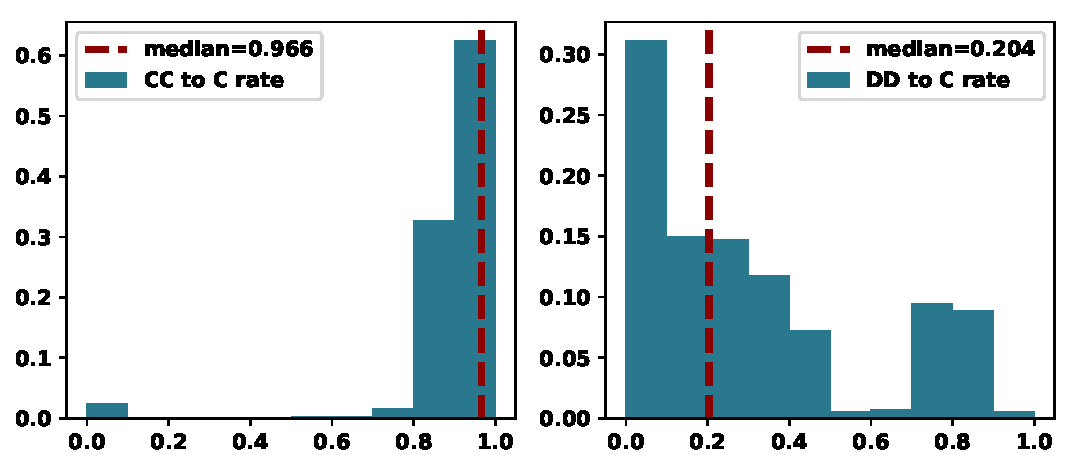
\includegraphics[width=.65\textwidth]{../images/rates_of_winners_in_standard_tournaments.pdf}
    \caption{Distributions of $CC$ to $C$ and $DD$ to $C$ for the winners in
    standard tournaments.}\label{fig:rates_of_winners_in_standard_tournaments}
\end{figure}

Compared to standard tournaments, in both noisy and in probabilistic ending
tournaments the higher the rates of cooperation the lower a strategy's success
and median score. A strategy would want to cooperate less than both
the mean and median cooperator in such settings. In probabilistic ending
tournaments the correlations coefficients have a larger values, indicating a
stronger effect. Thus a strategy will be punished more by it's cooperative
behaviour in probabilistic ending environments, this was seen in Section~\ref{section:evaluation_of_performance}
as well. The distributions of the $C_r$ of the winners in
both tournaments is given by Figure~\ref{fig:c_r_distributions}. It confirms
that the winners in noisy tournaments cooperated less than 35\% of the times
and in probabilistic ending tournaments less than 10\%.
In noisy probabilistic ending tournaments and in over all the tournaments' results,
the only features that had a moderate affect are $C_r/C_{\text{mean}},
C_r/C_{\text{max}}$ and $C_r$. In such environments cooperative behaviour
appears to be punished by not as much as in noisy and probabilistic ending
tournaments.

\begin{figure}[!htbp]
    \centering
    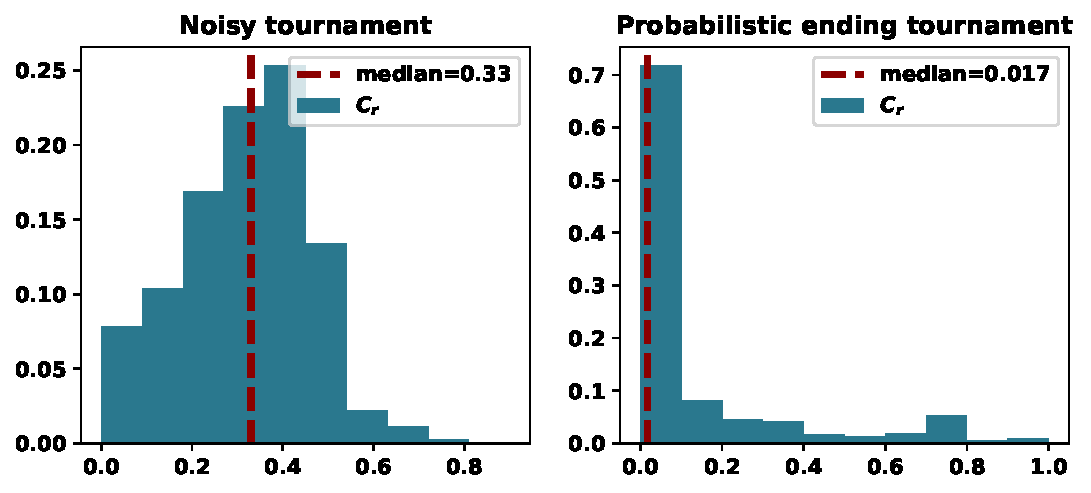
\includegraphics[width=.65\textwidth]{../images/c_r_winners_tournaments.pdf}
    \caption{$C_r$ distributions of the winners in noisy and in probabilistic
    ending tournaments.}\label{fig:c_r_distributions}
\end{figure}

The performances are clustered based on the normalised rank. More specifically,
they are clustered 3 times into 2 different clusters based on  on whether their
normalised rank was in the top 5\%, 25\% or 50\% respectively. A random forest
approach~\cite{breiman2001} is then applied to each performance to predict the cluster to
which it has been assigned to. The random forest method
constructs many individual decision trees and the predictions from all trees are
pooled to make the final prediction. The random forest models are trained on a
training set of 70\% of the tournaments results. The accuracy of each model
based on $R^2$ are given by Table~\ref{table:accuracy_random_forest}. The out of
the bag error (OOB)~\cite{hastie2005} has also been calculated. The models fit well,
and a high value of both the accuracy measure on the test data and the OOB error
indicate that the model is not over fitting.

The performances have also been clustered based on their normalised rank and
their median score by a \(k-\)means algorithm~\cite{Arthur2007}. The number of
clusters is not deterministically chosen but it is based on the silhouette
coefficients~\cite{Rousseeuw1987}. The chosen cluster for each tournament type,
as well as the accuracy for random forest models are also given in
Table~\ref{table:accuracy_random_forest}.

\begin{table}[!htbp]
    \begin{center}
        \resizebox{.9\textwidth}{!}{
        \begin{tabular}{lccccc}
    \toprule
    Tournament type & Clustering on & Number of clusters & $R^2$ training data &  $R^2$ test data  & $R^2$ OOB score\\
    \midrule
    standard  & top 5\% $r$              & 2  & 0.998831  & 0.987041 & 0.983708 \\
              & top 25\% $r$             & 2  & 0.998643  & 0.978626 & 0.969202 \\
              & top 50\% $r$             & 2  & 0.998417  & 0.985217 & 0.976538 \\
              & $r$  \& normalised score & 2  & 0.998794  & 0.990677 & 0.982959 \\
    \midrule
    noisy     & top 5\% $r$              & 2 & 0.996677  & 0.950572 & 0.935383\\
              & top 25\% $r$             & 2 & 0.996677  & 0.950572 & 0.935383\\
              & top 50\% $r$             & 2 & 0.996677  & 0.950572 & 0.935383\\
              & $r$  \& normalised score & 3 & 0.996677  & 0.950572 & 0.935383\\
    \midrule
    probabilistic ending & top 5\% $r$              & 2 & 0.999592  & 0.995128 & 0.992819 \\
                         & top 25\% $r$             & 2 & 0.999592  & 0.995128 & 0.992819 \\
                         & top 50\% $r$             & 2 & 0.999592  & 0.995128 & 0.992819 \\
                         & $r$  \& normalised score & 2 & 0.999592  & 0.995128 & 0.992819 \\
    \midrule
    noisy probabilistic ending & top 5\% $r$              & 2 & 0.990490  & 0.813905 & 0.791418\\
                               & top 25\% $r$             & 2 & 0.990490  & 0.813905 & 0.791418\\
                               & top 50\% $r$             & 2 & 0.990490  & 0.813905 & 0.791418\\
                               & $r$  \& normalised score & 4 & 0.990490  & 0.813905 & 0.791418\\
    \midrule
    over \numberofalltournaments tournaments & top 5\% $r$               & 2 & 0.993396 & 0.913409 & 0.898059 \\
                                             & top 25\% $r$              & 2 & 0.993396 & 0.913409 & 0.898059 \\
                                             & top 50\% $r$              & 2 & 0.993396 & 0.913409 & 0.898059 \\
                                             & $r$  \& normalised score  & 3 & 0.993396 & 0.913409 & 0.898059 \\
    \bottomrule
        \end{tabular}}
    \end{center}
    \caption{Accuracy metrics for random forest models.}
    \label{table:accuracy_random_forest}
\end{table}

The importance that the features of Table~\ref{table:manual_features} had on
each classification task; to which cluster a performance was assigned to based
on the normalised rank, and their normalised rank and median score have been
calculated and are given by Figures~\ref{fig:clustering_importance_standard},
\ref{fig:clustering_importance_noise},~\ref{fig:clustering_importance_probend},
\ref{fig:clustering_importance_probend_noise}
and~\ref{fig:clustering_importance_overall}. These show that the classifiers
stochastic, make use of game and make use of length have no significant effect,
and several of the features that are highted by the importance are inline with
the correlation results. Moreover, the smoothing parameter \(k\) appears to no
have a significant effect either. The most important features based on the
random forest analysis were $C_{r} / C_{median}$ and $C_r / C_{mean}$.

\begin{figure}[!htbp]
    \begin{subfigure}[t]{0.5\textwidth}
        \begin{center}
            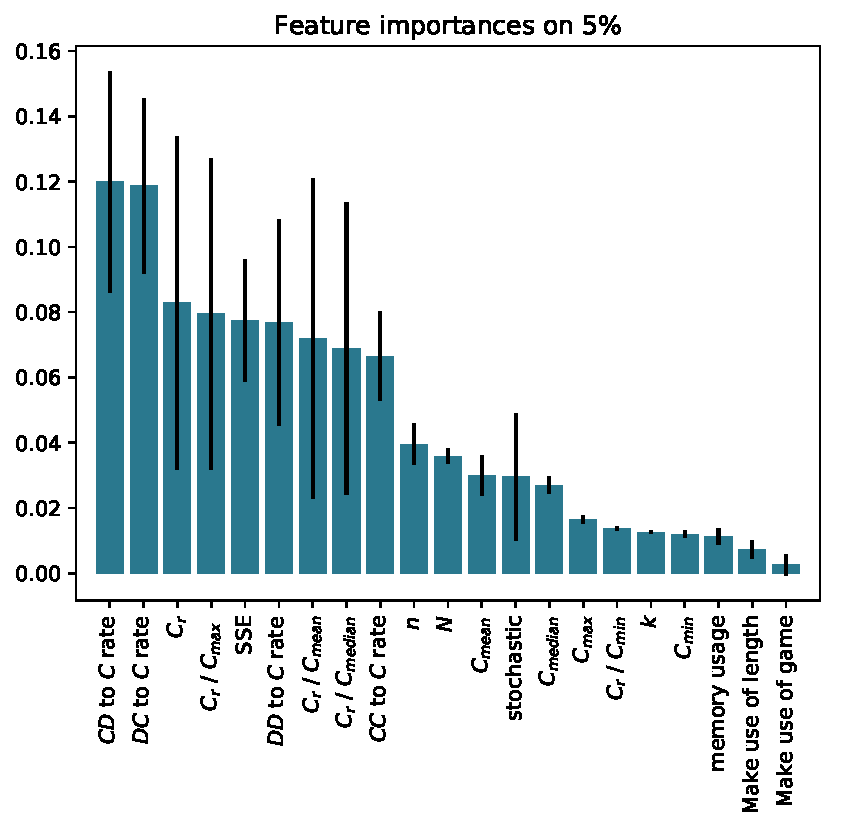
\includegraphics[width=.75\linewidth]{../new_output/standard/_feature_importance_bar_plot_cluster_on_0_05.pdf}
        \end{center}
        \caption{Importance of features for clusters on 5\% performance.}
    \end{subfigure}\hfill
    \begin{subfigure}[t]{0.5\textwidth}
        \begin{center}
            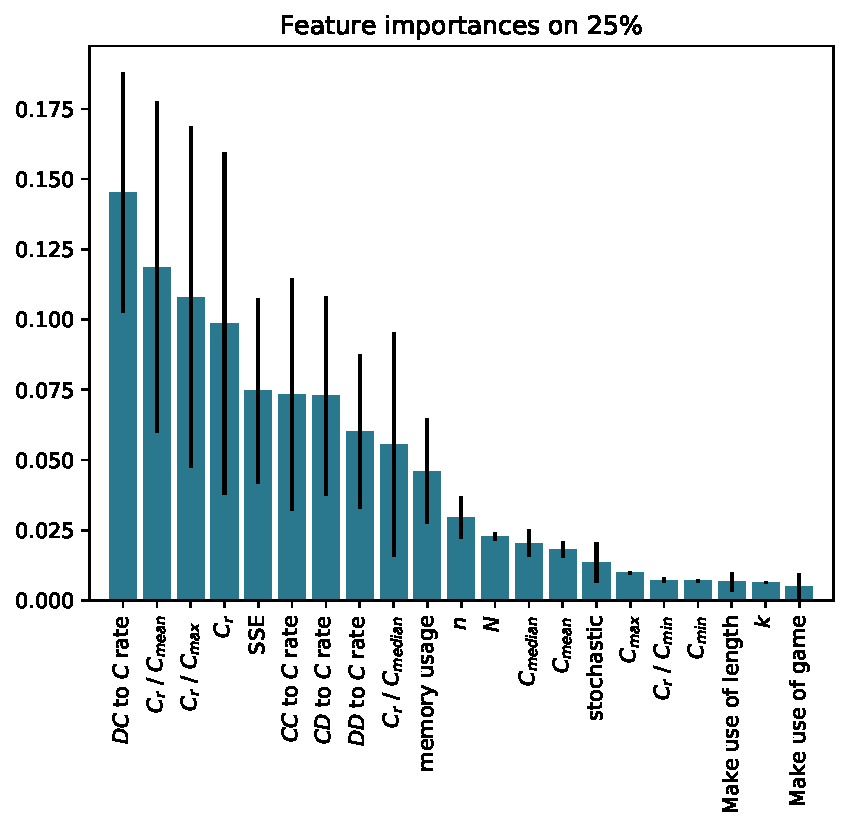
\includegraphics[width=.75\linewidth]{../new_output/standard/_feature_importance_bar_plot_cluster_on_0_25.pdf}
        \end{center}
        \caption{Importance of features for clusters on 25\% performance.}
    \end{subfigure}
    \begin{subfigure}[t]{0.5\textwidth}
        \begin{center}
            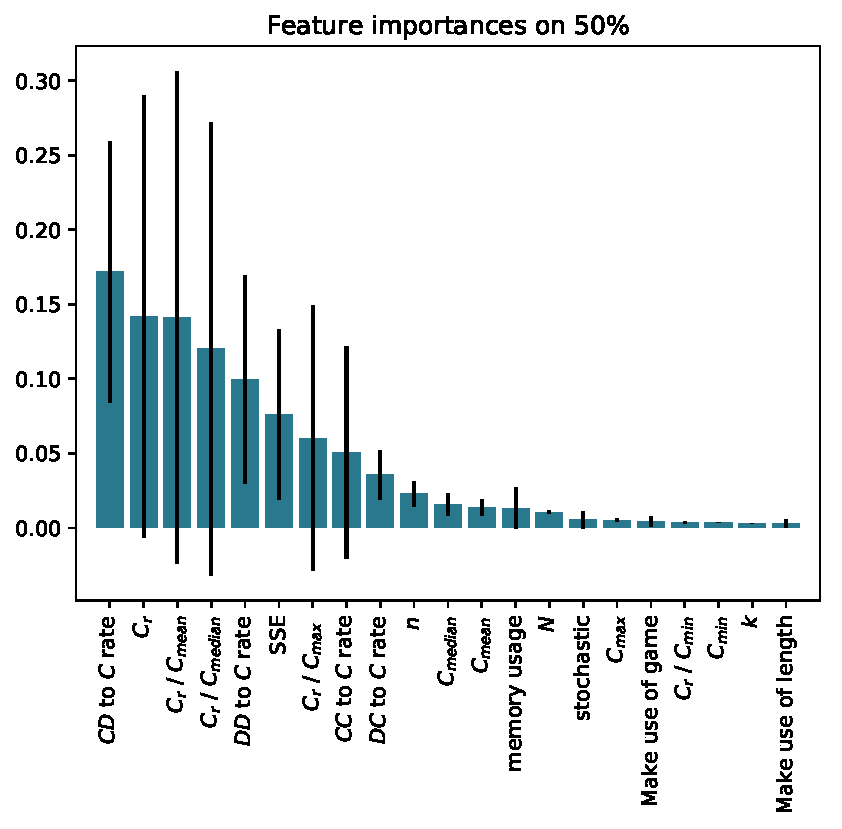
\includegraphics[width=.75\linewidth]{../new_output/standard/_feature_importance_bar_plot_cluster_on_0_5.pdf}
        \end{center}
        \caption{Importance of features for clusters on 50\% performance.}
    \end{subfigure}\hfill
    \begin{subfigure}[t]{0.5\textwidth}
        \begin{center}
            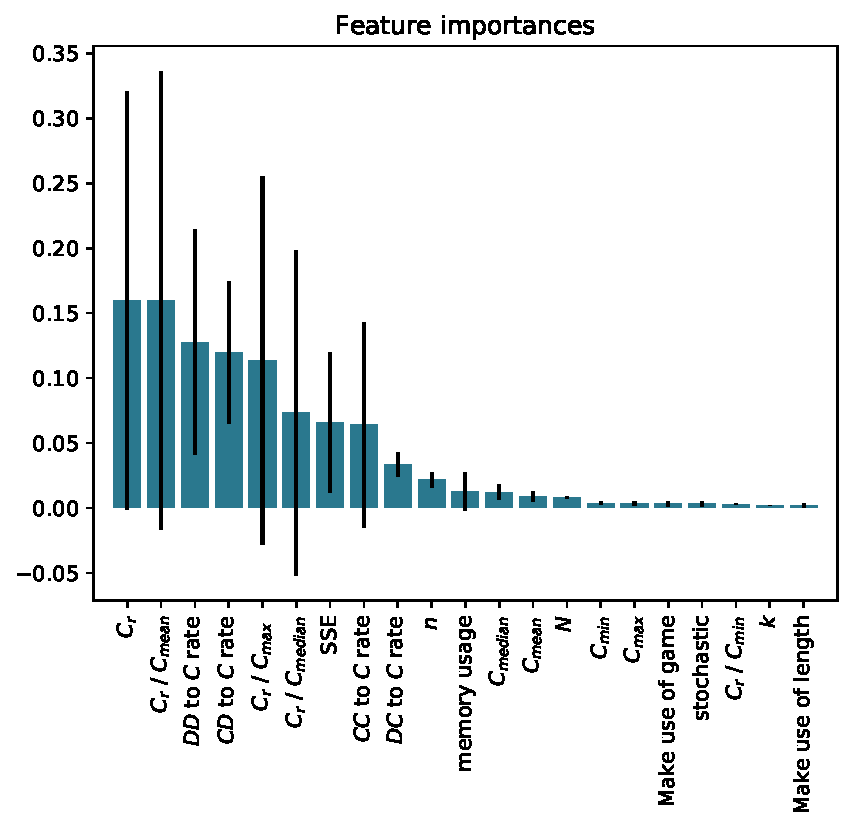
\includegraphics[width=.75\linewidth]{../k_means_output/standard/_feature_importance_bar_plot.pdf}
        \end{center}
        \caption{Importance of features for clusters based on \(k\)means algorithm.}
    \end{subfigure}
    \caption{Importance of features in standard tournaments for different
    clustering methods.}\label{fig:clustering_importance_standard}
\end{figure}

\begin{figure}[!htbp]
    \begin{subfigure}{0.5\textwidth}
        \begin{center}
            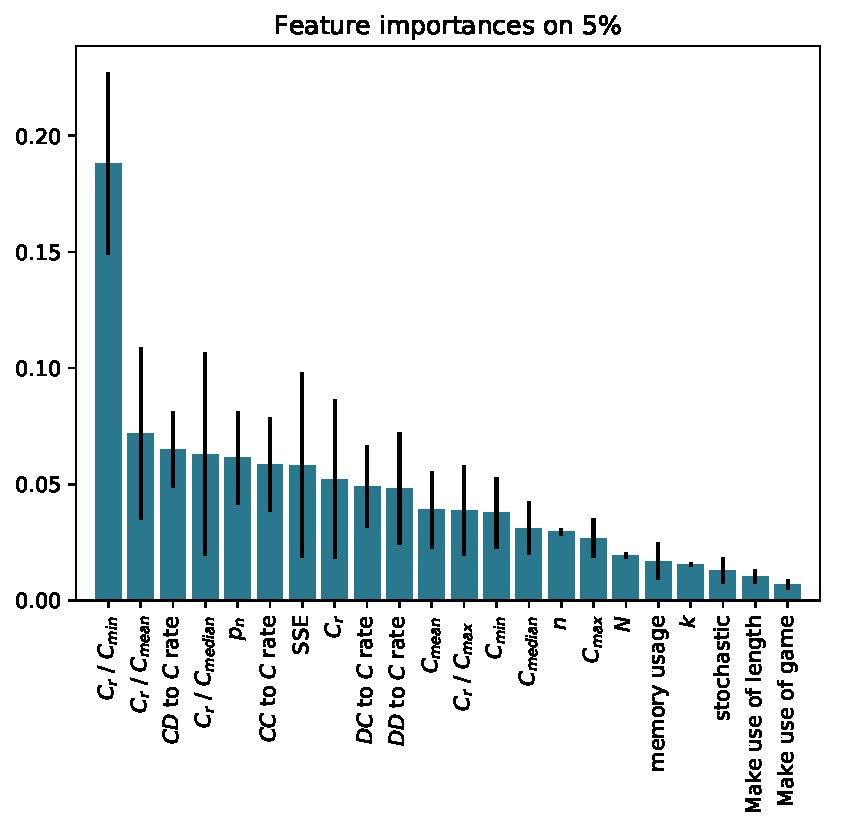
\includegraphics[width=.75\linewidth]{../new_output/noise/_feature_importance_bar_plot_cluster_on_0_05.pdf}
        \end{center}
        \caption{Importance of features for clusters on 5\% performance.}
    \end{subfigure}\hfill
    \begin{subfigure}{0.5\textwidth}
        \begin{center}
            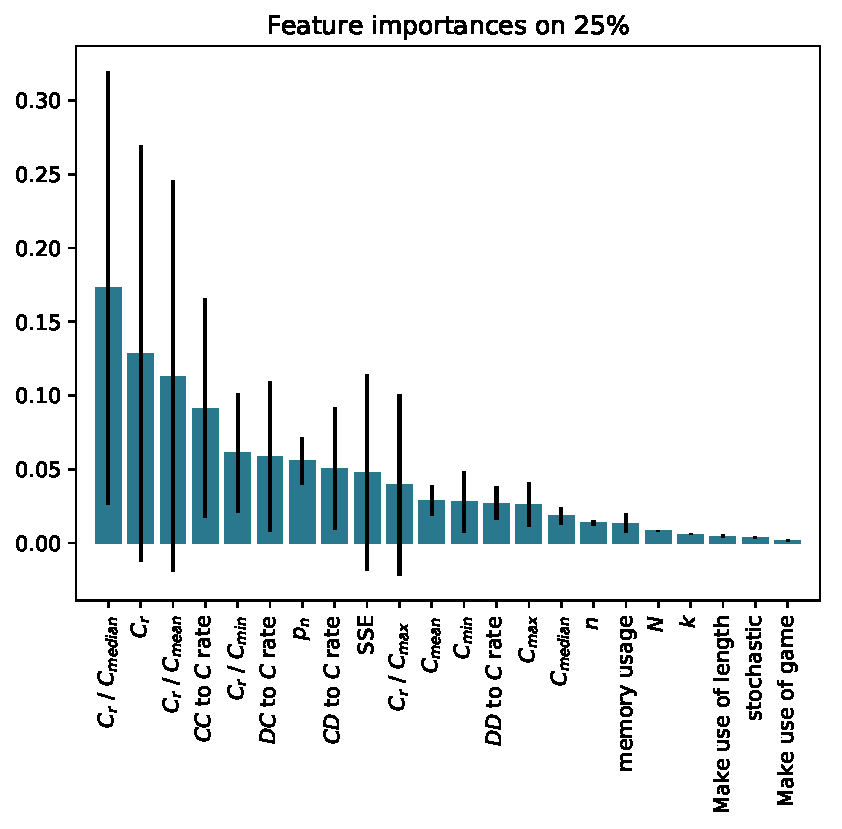
\includegraphics[width=.75\linewidth]{../new_output/noise/_feature_importance_bar_plot_cluster_on_0_25.pdf}
        \end{center}
        \caption{Importance of features for clusters on 25\% performance.}
    \end{subfigure}
    \begin{subfigure}{0.5\textwidth}
        \begin{center}
            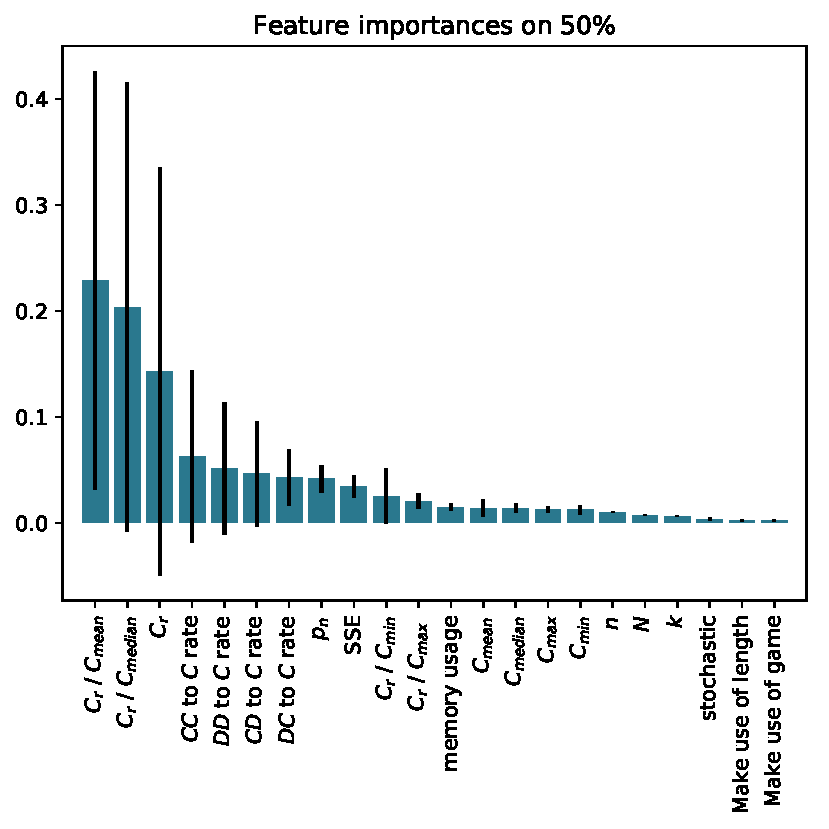
\includegraphics[width=.75\linewidth]{../new_output/noise/_feature_importance_bar_plot_cluster_on_0_5.pdf}
        \end{center}
        \caption{Importance of features for clusters on 50\% performance.}
    \end{subfigure}\hfill
    \begin{subfigure}{0.5\textwidth}
        \begin{center}
            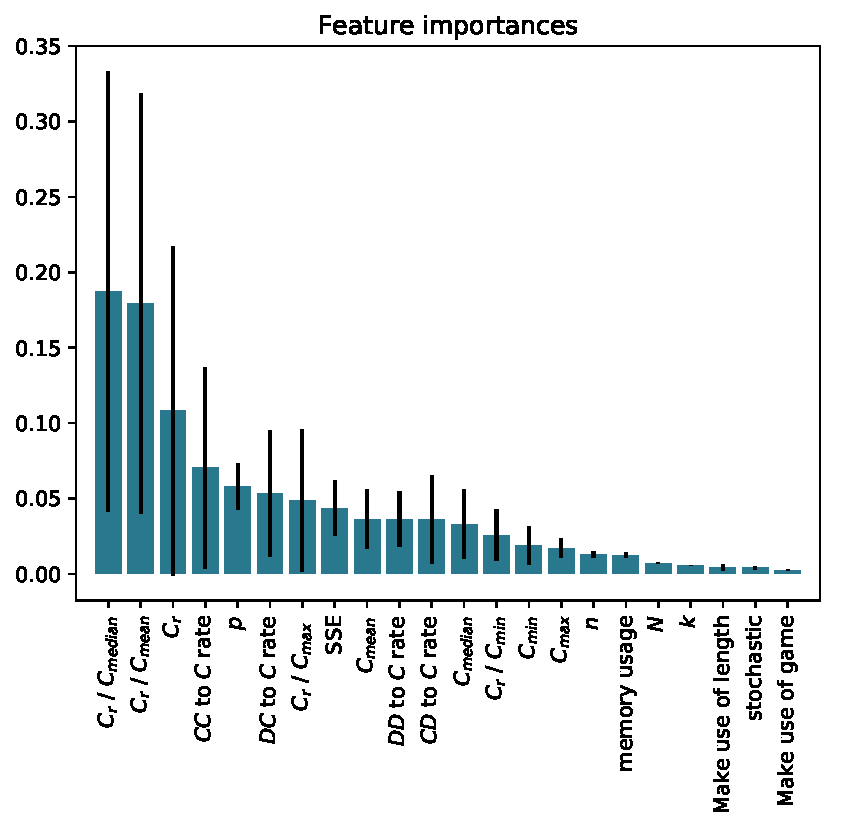
\includegraphics[width=.75\linewidth]{../k_means_output/noise/_feature_importance_bar_plot.pdf}
        \end{center}
        \caption{Importance of features for clusters based on \(k\)means algorithm.}
    \end{subfigure}
    \caption{Importance of features in noisy tournaments for different
    clustering methods.}\label{fig:clustering_importance_noise}
\end{figure}

\begin{figure}[!htbp]
    \begin{subfigure}[t]{0.5\textwidth}
        \begin{center}
            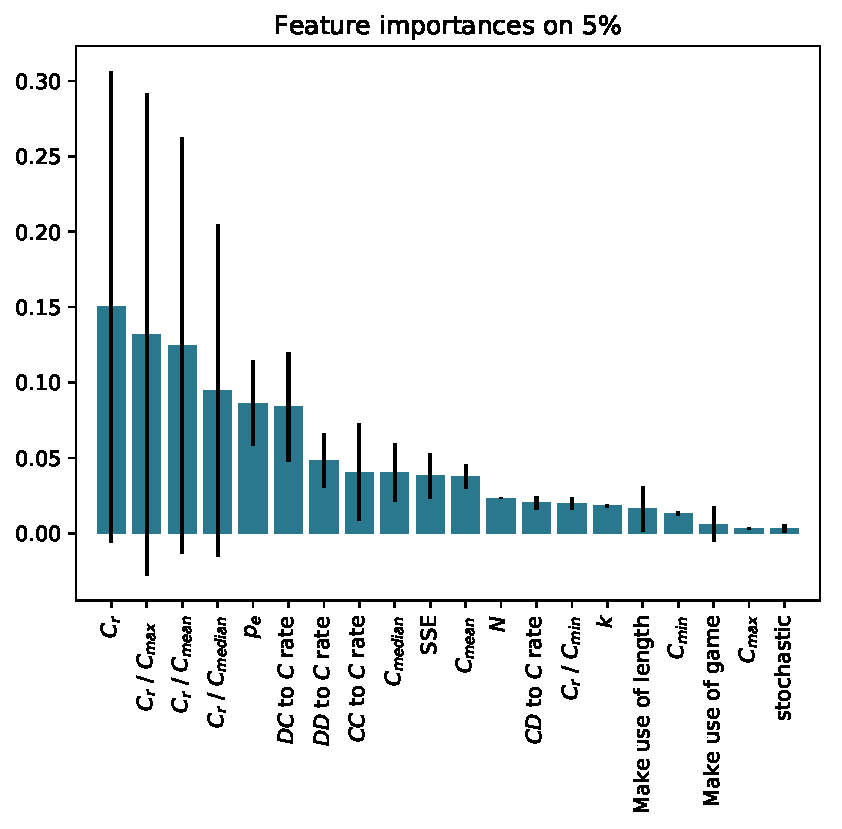
\includegraphics[width=.75\linewidth]{../new_output/probend/_feature_importance_bar_plot_cluster_on_0_05.pdf}
        \end{center}
        \caption{Importance of features for clusters on 5\% performance.}
    \end{subfigure}
    \begin{subfigure}[t]{0.5\textwidth}
        \begin{center}
            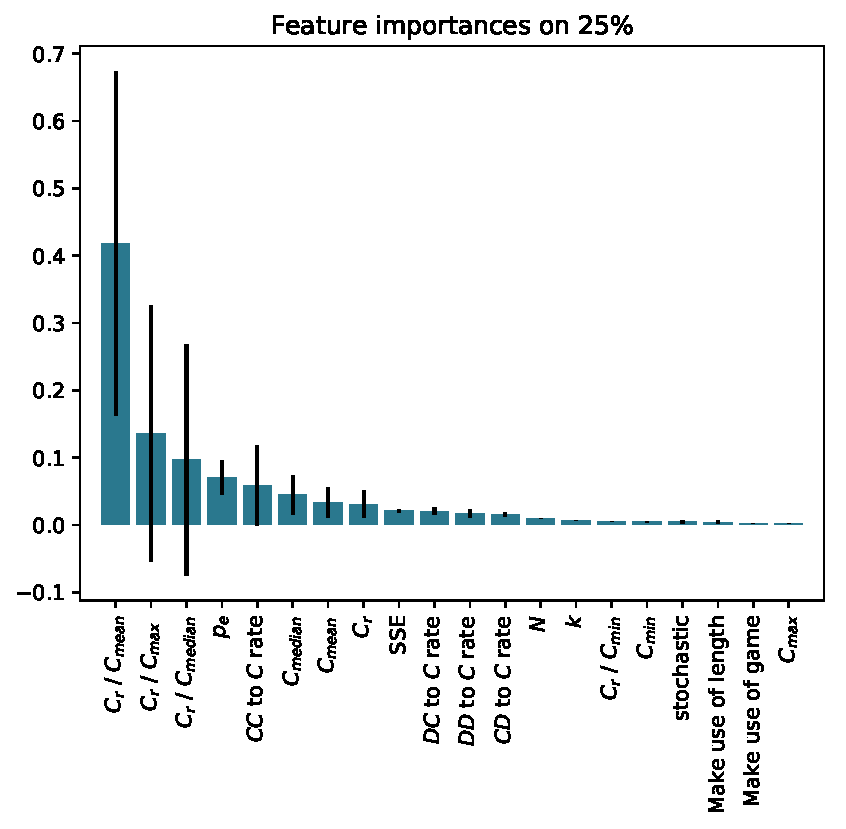
\includegraphics[width=.75\linewidth]{../new_output/probend/_feature_importance_bar_plot_cluster_on_0_25.pdf}
        \end{center}
        \caption{Importance of features for clusters on 25\% performance.}
    \end{subfigure}
    \begin{subfigure}[t]{0.5\textwidth}
        \begin{center}
            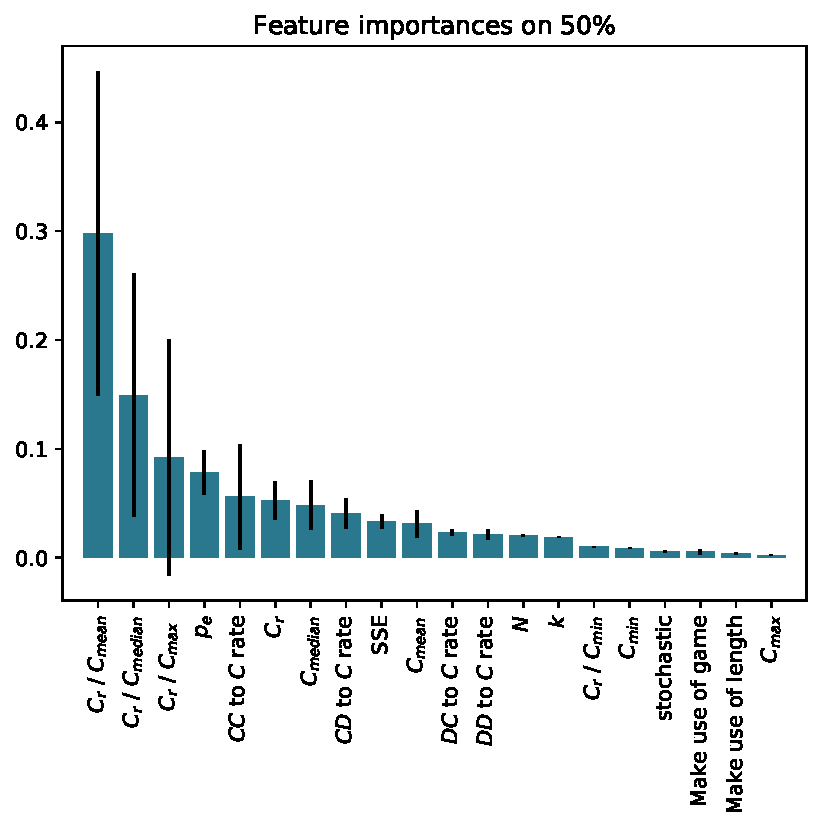
\includegraphics[width=.75\linewidth]{../new_output/probend/_feature_importance_bar_plot_cluster_on_0_5.pdf}
        \end{center}
        \caption{Importance of features for clusters on 50\% performance.}
    \end{subfigure}
    \begin{subfigure}[t]{0.5\textwidth}
        \begin{center}
            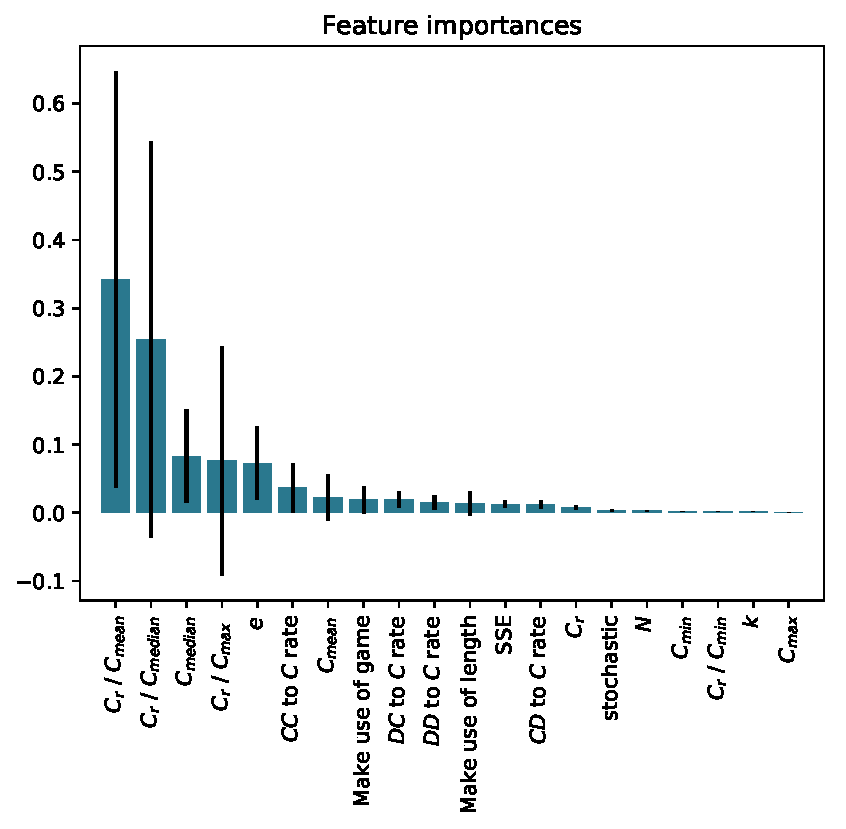
\includegraphics[width=.75\linewidth]{../k_means_output/probend/_feature_importance_bar_plot.pdf}
        \end{center}
        \caption{Importance of features for clusters based on \(k\)means algorithm.}
    \end{subfigure}
    \caption{Importance of features in probabilistic ending tournaments for different
    clustering methods.}\label{fig:clustering_importance_probend}
\end{figure}

\begin{figure}[!htbp]
    \begin{subfigure}[t]{0.5\textwidth}
        \begin{center}
            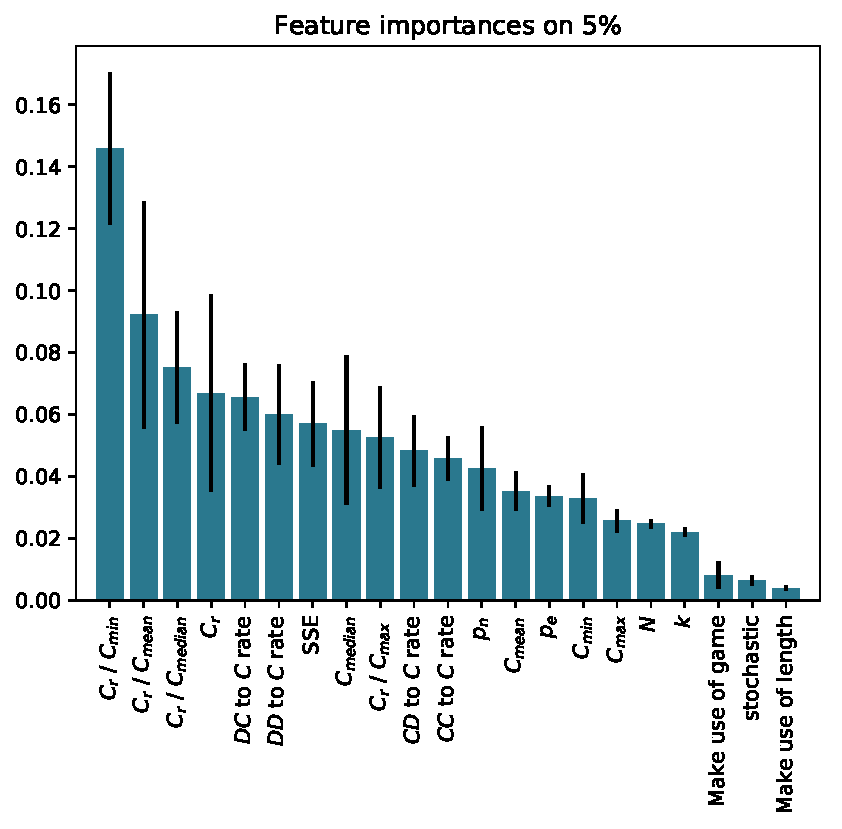
\includegraphics[width=.75\linewidth]{../new_output/probend_noise/_feature_importance_bar_plot_cluster_on_0_05.pdf}
        \end{center}
        \caption{Importance of features for clusters on 5\% performance.}
    \end{subfigure}
    \begin{subfigure}[t]{0.5\textwidth}
        \begin{center}
            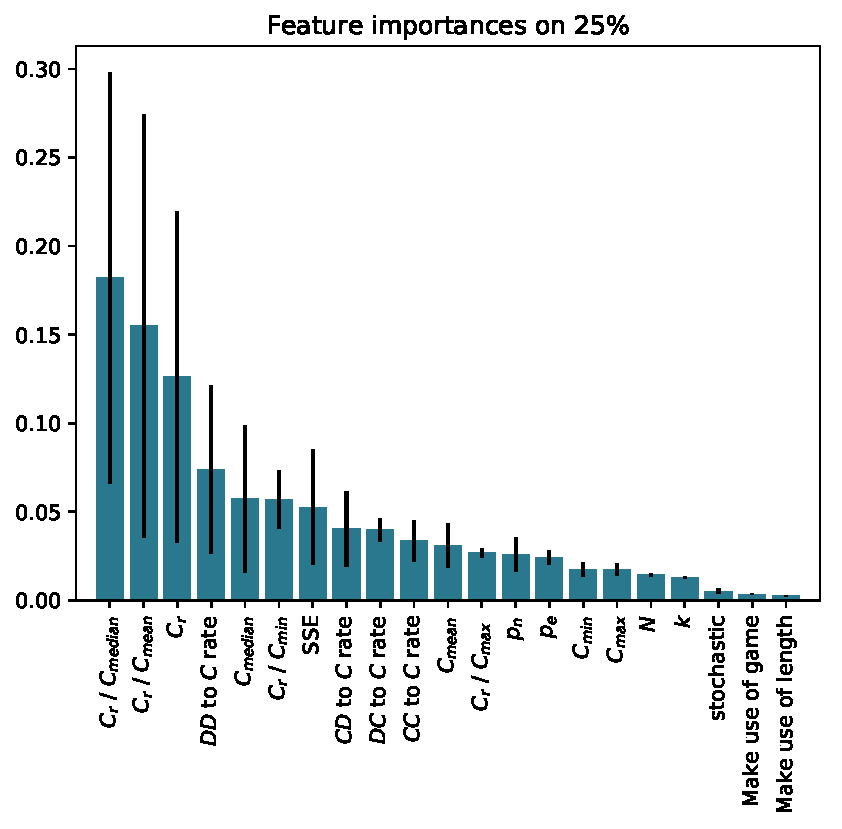
\includegraphics[width=.75\linewidth]{../new_output/probend_noise/_feature_importance_bar_plot_cluster_on_0_25.pdf}
        \end{center}
        \caption{Importance of features for clusters on 25\% performance.}
    \end{subfigure}
    \begin{subfigure}[t]{0.5\textwidth}
        \begin{center}
            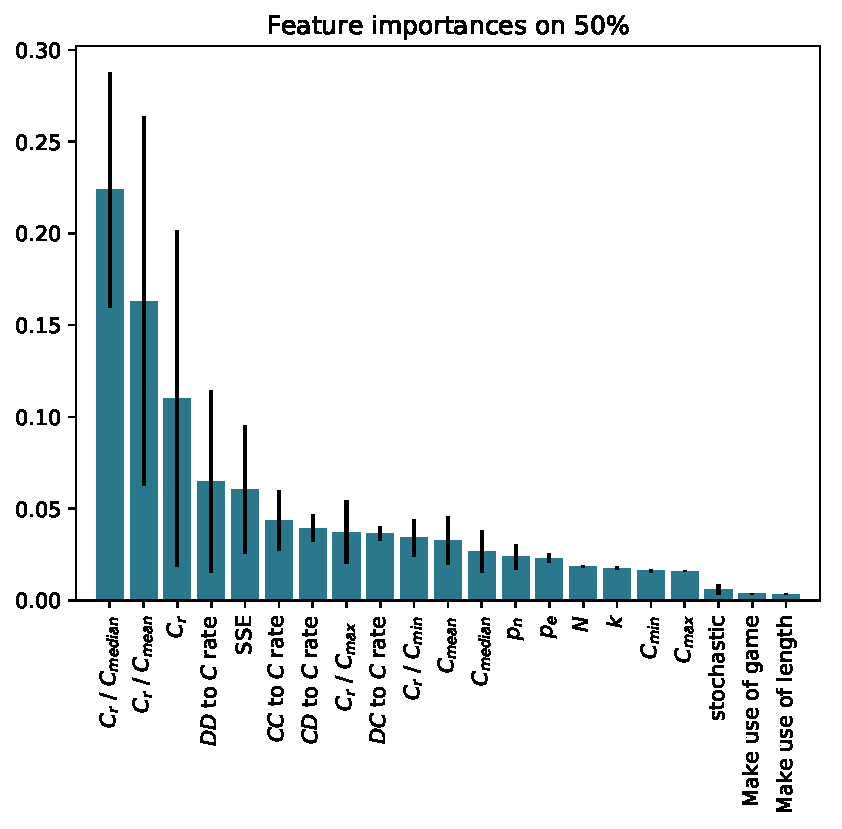
\includegraphics[width=.75\linewidth]{../new_output/probend_noise/_feature_importance_bar_plot_cluster_on_0_5.pdf}
        \end{center}
        \caption{Importance of features for clusters on 50\% performance.}
    \end{subfigure}
    \begin{subfigure}[t]{0.5\textwidth}
        \begin{center}
            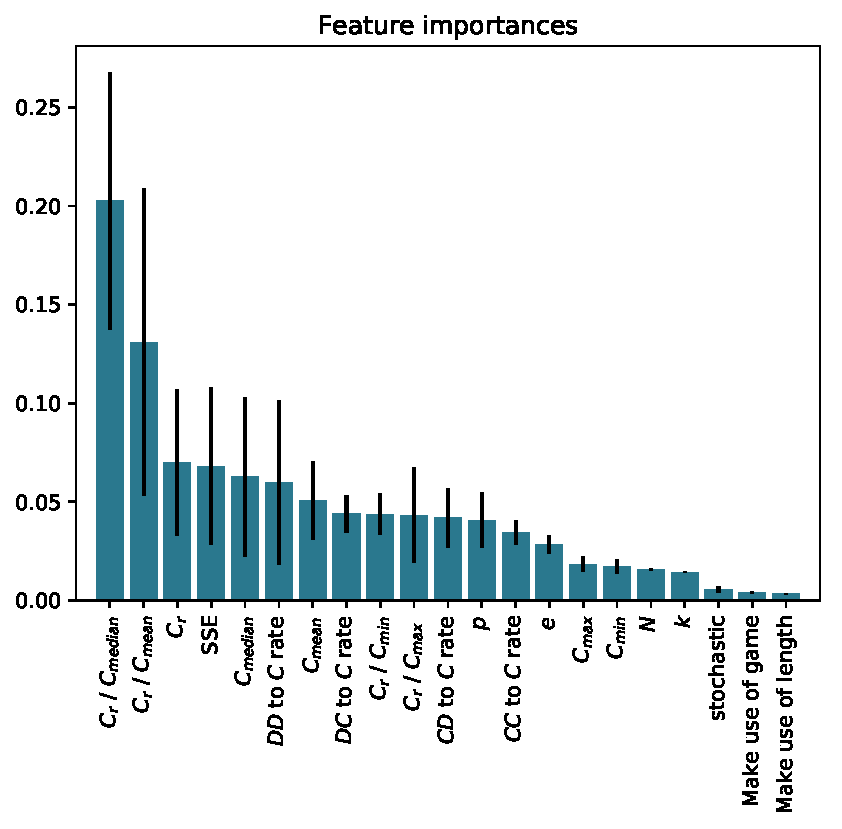
\includegraphics[width=.75\linewidth]{../k_means_output/probend_noise/_feature_importance_bar_plot.pdf}
        \end{center}
        \caption{Importance of features for clusters based on \(k\)means algorithm.}
    \end{subfigure}
    \caption{Importance of features in noisy probabilistic ending tournaments for different
    clustering methods.}\label{fig:clustering_importance_probend_noise}
\end{figure}

\begin{figure}[!htbp]
    \begin{subfigure}[t]{0.5\textwidth}
        \begin{center}
            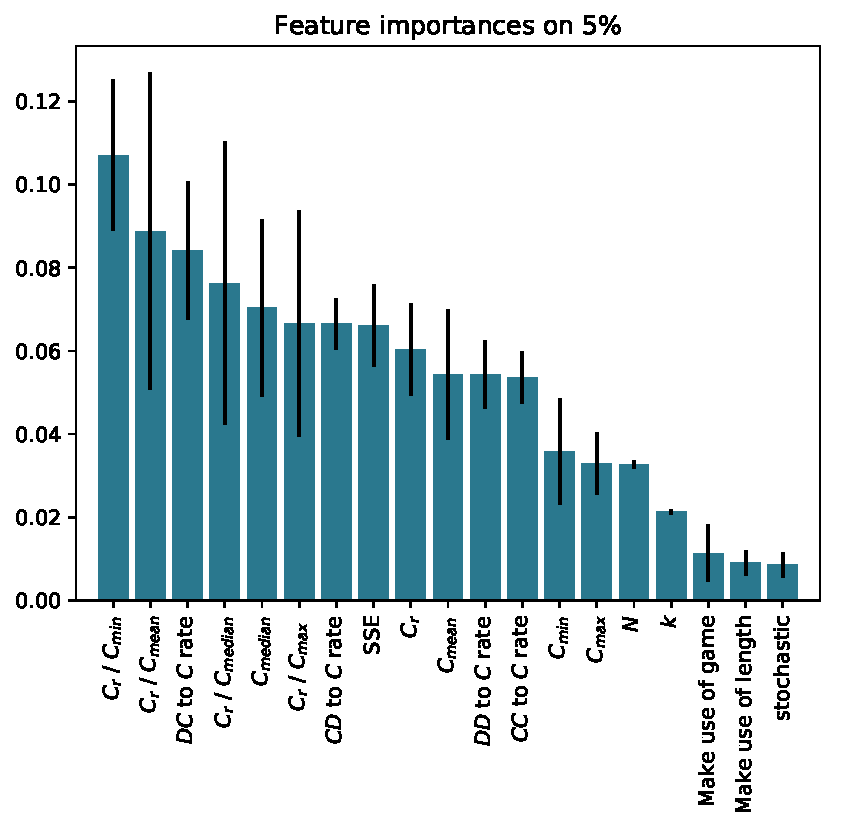
\includegraphics[width=.75\linewidth]{../new_output/merged/_feature_importance_bar_plot_cluster_on_0_05.pdf}
        \end{center}
        \caption{Importance of features for clusters on 5\% performance.}
    \end{subfigure}
    \begin{subfigure}[t]{0.5\textwidth}
        \begin{center}
            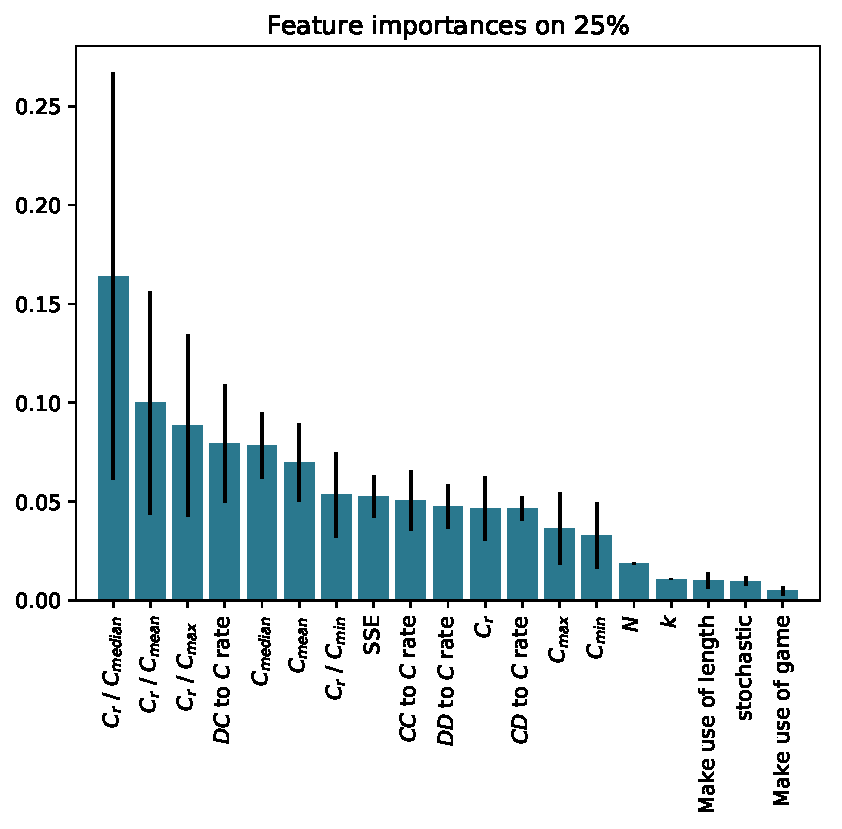
\includegraphics[width=.75\linewidth]{../new_output/merged/_feature_importance_bar_plot_cluster_on_0_25.pdf}
        \end{center}
        \caption{Importance of features for clusters on 25\% performance.}
    \end{subfigure}
    \begin{subfigure}[t]{0.5\textwidth}
        \begin{center}
            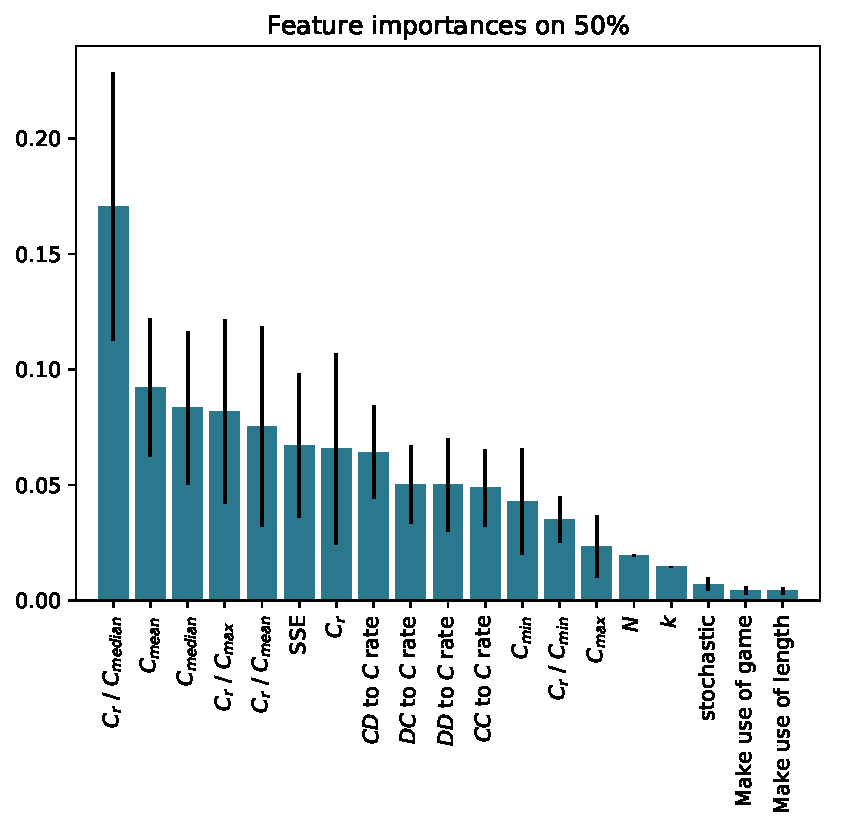
\includegraphics[width=.75\linewidth]{../new_output/merged/_feature_importance_bar_plot_cluster_on_0_5.pdf}
        \end{center}
        \caption{Importance of features for clusters on 50\% performance.}
    \end{subfigure}
    \begin{subfigure}[t]{0.5\textwidth}
        \begin{center}
            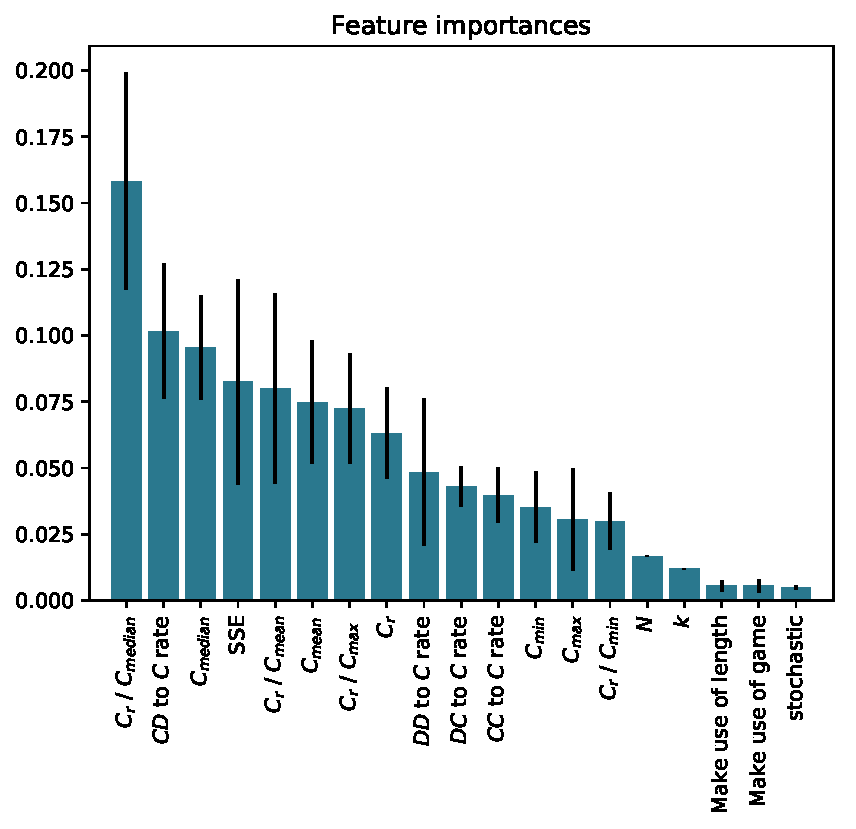
\includegraphics[width=.75\linewidth]{../k_means_output/merged/_feature_importance_bar_plot.pdf}
        \end{center}
        \caption{Importance of features for clusters based on \(k\)means algorithm.}
    \end{subfigure}
    \caption{Importance of features over all the tournaments for different
    clustering methods.}\label{fig:clustering_importance_overall}
\end{figure}

The effect of both these features can be further explored. In
Figure~\ref{fig:mean_median_std} the distributions of \(C_r / C_{\text{mean}}\)
and \(C_r / C_{\text{median}}\) are given for the winners in standard tournaments. A value of \(C_r /
C_{\text{mean}} = 1\) imply that the cooperating ratio of the winner was the
same as the mean/median cooperating ratio of the tournament. In standard tournaments, the mean
for both ratios is 1. Therefore, an effective strategy in standard tournaments
was the mean/median cooperator of its respective tournament. In comparison,
Figure~\ref{fig:mean_median_noisy} shows the distributions of the features for
the winners in noisy tournaments where the mean is at 0.67. Thereupon the winners
cooperated 67\% of the times the mean/median cooperator did. This analysis is
applied to the rest of the tournaments and the distributions are given by
Figures \ref{fig:mean_median_probend}, \ref{fig:mean_median_probend_noisy} and
\ref{fig:mean_median_overall}. In a tournament with noisy and a probabilistic
ending the winners cooperated 60\%, whereas in settings that the type of the
tournament can vary between the types considered in this work the winners
cooperated 67\% of the times the mean or median cooperator did. Finally, in
probabilistic ending tournament it has already been mentioned that defecting
strategies prevail and this result is once again confirmed in this section.

\begin{figure}[!htbp]
    \centering
    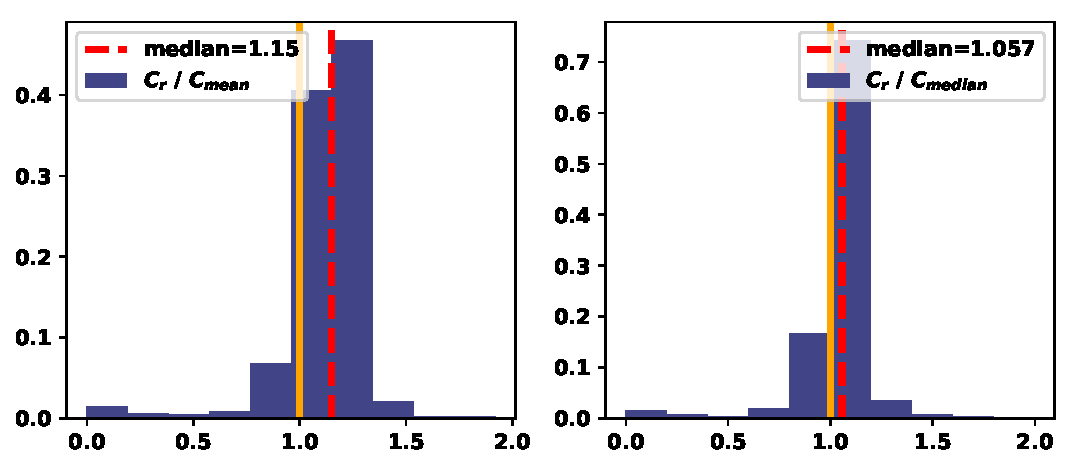
\includegraphics[width=.5\textwidth]{../images/compared_to_mean_median_standard.pdf}
    \caption{Distributions of \(C_r / C_{\text{median}}\)
    and \(C_r / C_{\text{median}}\) for winners of standard tournaments.}\label{fig:mean_median_std}
\end{figure}

\begin{figure}[!htbp]
    \centering
    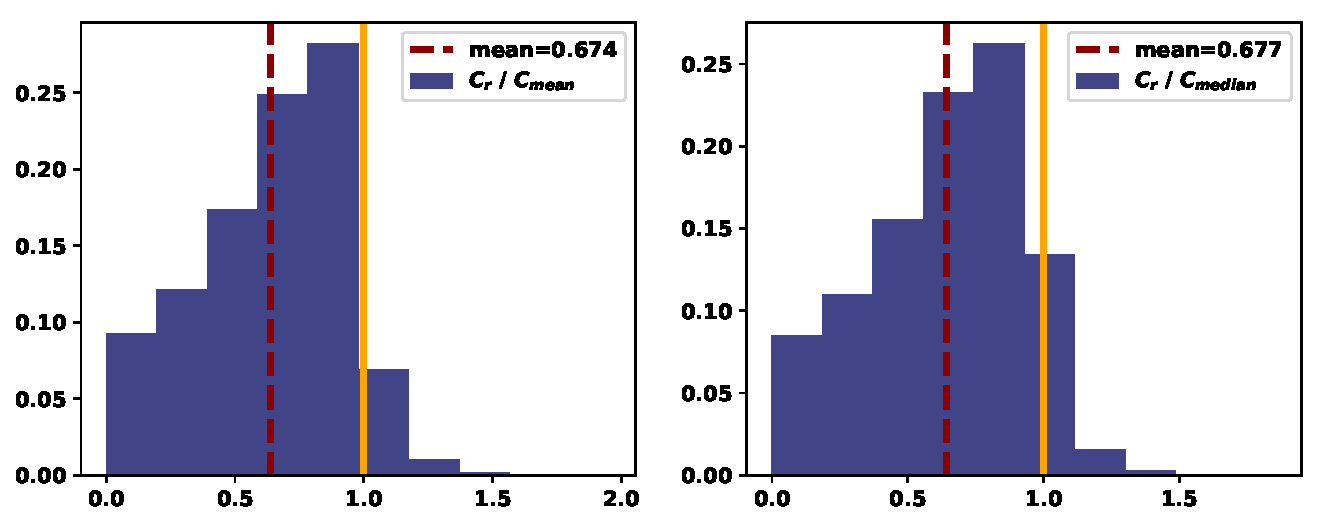
\includegraphics[width=.5\textwidth]{../images/compared_to_mean_median_noisy.pdf}
    \caption{Distributions of \(C_r / C_{\text{median}}\)
    and \(C_r / C_{\text{median}}\) for winners of noisy tournaments.}\label{fig:mean_median_noisy}
\end{figure}

\begin{figure}[!htbp]
    \centering
    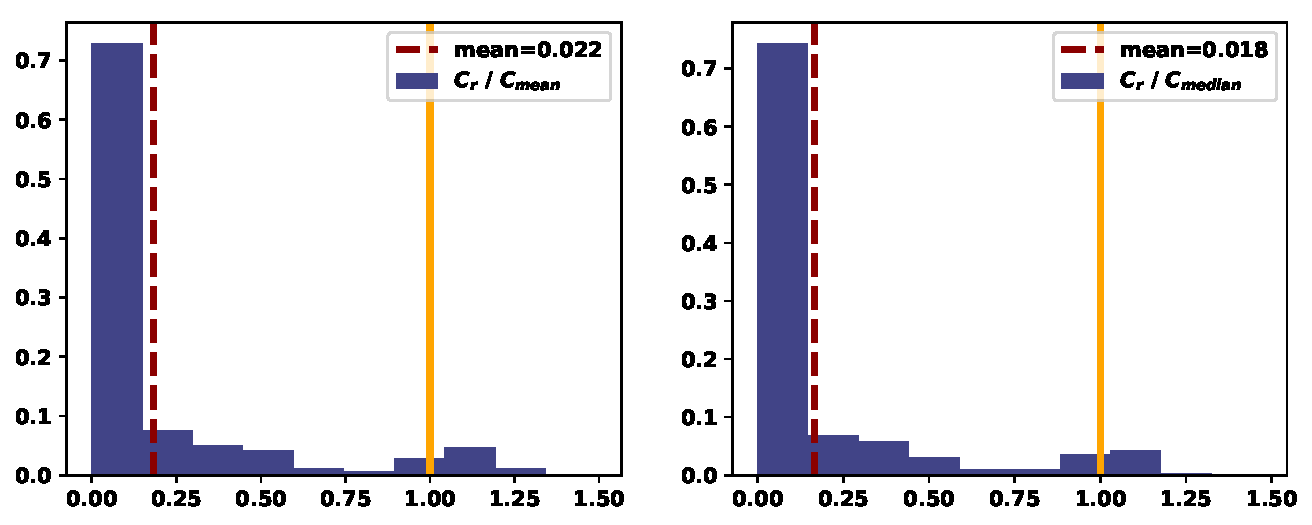
\includegraphics[width=.5\textwidth]{../images/compared_to_mean_median_probend.pdf}
    \caption{Distributions of \(C_r / C_{\text{median}}\)
    and \(C_r / C_{\text{median}}\) for winners of probabilistic ending tournaments.}\label{fig:mean_median_probend}
\end{figure}

\begin{figure}[!htbp]
    \centering
    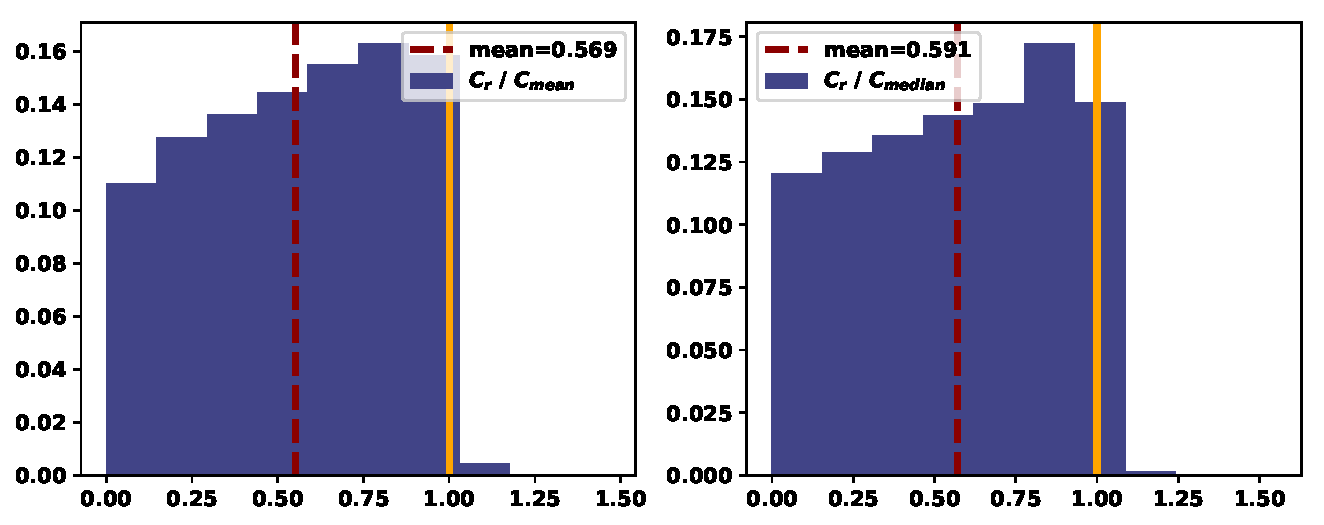
\includegraphics[width=.5\textwidth]{../images/compared_to_mean_median_probend_noisy.pdf}
    \caption{Distributions of \(C_r / C_{\text{median}}\)
    and \(C_r / C_{\text{median}}\) for winners of noisy probabilistic ending tournaments.}\label{fig:mean_median_probend_noisy}
\end{figure}

\begin{figure}[!htbp]
    \centering
    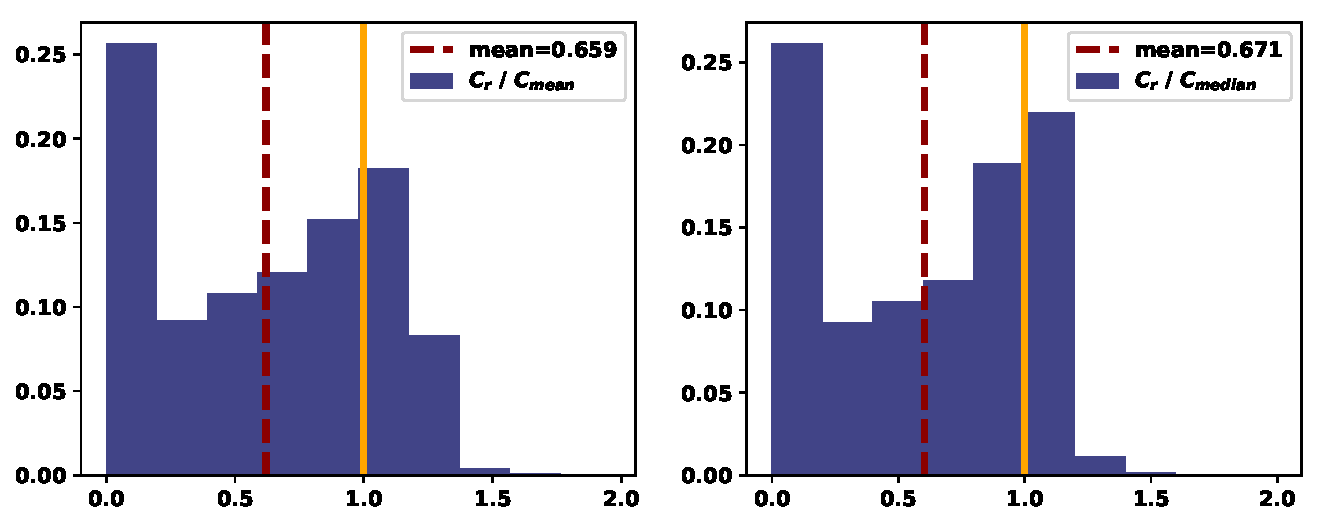
\includegraphics[width=.5\textwidth]{../images/compared_to_mean_median_overall.pdf}
    \caption{Distributions of \(C_r / C_{\text{median}}\)
    and \(C_r / C_{\text{median}}\) for winners of over all the tournaments.}\label{fig:mean_median_overall}
\end{figure}

In this section the effect of several features, regarding a strategy's behaviour
and the tournament in which it participated on its performance were presented.
This was done using two approaches. Correlation coefficients and a random forest
analysis. The results of these are summarised in the following section.

\section{Conclusion}\label{section:conclusion}

This manuscript has explored the performance of \numberofstrategies strategies of the Iterated
Prisoner's Dilemma in a large number of computer tournaments. The results of
the analysis demonstrated that, although for specific tournament types such as
standard and probabilistic ending tournaments, dominant strategies exist
there is not a single dominant type of strategies if the environments
vary. Moreover, a strategy with a theory of mind should aim to adapt its behaviour
based on the mean and median cooperators.

The \numberofstrategies strategies used in this manuscript have been mainly from
the literature, and they have been accessible due to an open source software
called Axelrod-Python library. The software was used to generate a total of
\numberofalltournaments computer tournaments results with different number of
strategies and different participants each time. The data collection was
described in Section~\ref{section:data_collection}. In
Section~\ref{section:top_performances}, the tournaments results were used to
present the top performances. The data set contained results from four different
settings, and these were also studied individually. In standard tournaments
complex strategies trained using reinforcement learning ranked in the top spots.
Some of these strategies ranked again in the top spots in probabilistic
ending tournaments when a \(p_e\) of less 0.1 was considered. In probabilistic
ending tournaments \(p_e\) was designed to vary between 0 and 1. It was demonstrated
that for values larger than 0.1, as stated in the Folk Theorem, defecting strategies
were winning the tournaments because there was a high likelihood of the game
ending in the next turn. In tournaments with noise the median ranks of the top
15 strategies had the highest values and the \(r\) distributions were bimodal.
The top rank strategies were performing both well and bad, and this indicates
that in noisy tournaments there are not strategies that can guarantee winning.
Overall, the top ranked strategies differed from one tournament type to
another and the mechanism behind the winning strategies were all different.
Even strategies designed to do good in one setting did better in others.
On the whole ... (the ipd interactions are unique and there is no winning
strategy) %TODO help from Vince

Section~\ref{section:evaluation_of_performance}, covered an analysis of
performance based on several features associated with a strategy and with the
environments it was competing. The results of this analysis showed that a
strategy's characteristics such as whether or not it's stochastic, and the information it
used regarding the game had no effect on the strategy's success. The most
important features have been those that compared the strategy's behaviour to it's
environment. The cooperating ratio of the strategy compared to the mean and
median cooperator was highlighted as the most important feature in the analysis.
More specifically, if a strategy were to enter a tournament with a theory of
mind of its environment it would choose to be the median cooperator in standard
tournaments, to cooperate 10\% of the times the median cooperator did in probabilistic ending tournaments and 
60\% in noisy and noisy probabilistic
tournaments. Lastly, if a strategy was aware of the opponents but not of the
setting on the tournament, a strategy would be more likely to be successful if
it were to identify the median cooperator and cooperated 67\% of the times that
they did.

The data set described in this work contains the largest number of IPD tournaments,
to the authors knowledge, and available at~\cite{data}. Further data mining
could be applied and provide new insights in the field.

\bibliographystyle{plain}
\bibliography{bibliography}

\section{Acknowledgements}

A variety of software have been used in this work:

\begin{itemize}
    \item The Axelrod-Python library for IPD simulations~\cite{axelrodproject}.
    \item The Matplotlib library for visualisation~\cite{hunter2007matplotlib}.
    \item The Numpy library for data manipulation~\cite{walt2011numpy}.
    \item The scikit-learn library for data analysis~\cite{scikit-learn}.
\end{itemize}

\appendix

\section{A summary of parameters}\label{app:parameters}

A summary of the parameters and features used in this work are given
by Table~\ref{table:parameters_summary}.


\begin{table}[h]
    \begin{center}
    \resizebox{.7\textwidth}{!}{
    \begin{tabular}{llc}
    \toprule
feature & feature explanation \\
 \midrule
stochastic                  & If a strategy is stochastic \\
makes use of game           & If a strategy makes used of the game information  \\
makes use of length         & If a strategy makes used of the number of turns \\
memory usage                & The memory size of a strategy divided by the number of turns \\
SSE                         & A measure of how far a strategy is from extortionate behaviour \\
$C_{\text{max}}$          & The biggest cooperating rate in the tournament \\
$C_{\text{min}}$          & The smallest cooperating rate in the tournament \\
$C_{\text{median}}$       & The median cooperating rate in the tournament \\
$C_{\text{mean}}$         & The mean cooperating rate in the tournament \\
$C_r$ / $C_{\text{max}}$    & A strategy's cooperating rate divided by the maximum \\
$C_r$ / $C_{\text{min}}$    & A strategy's cooperating rate divided by the minimum \\
$C_r$ / $C_{\text{median}}$ & A strategy's cooperating rate divided by the median \\
$C_r$ / $C_{\text{mean}}$   & A strategy's cooperating rate divided by the mean \\
$C_r$                       & The cooperating ratio of a strategy \\
$CC$ to $C$ rate            & The probability a strategy will cooperate after a mutual cooperation \\
$CD$ to $C$ rate            & The probability a strategy will cooperate after being betrayed by the opponent \\
$DC$ to $C$ rate            & The probability a strategy will cooperate after betraying the opponent\\
$DD$ to $C$ rate            & The probability a strategy will cooperate after a mutual defection\\
$p_n$                       & The probability of a player's action being flip at each interaction \\
$n$                         & The number of turns \\
$p_e$                       & The probability of a match ending in the next turn \\
$N$                         & The number of strategies in the tournament \\
$k$                         & The number that a given tournament is repeated \\
    \bottomrule
        \end{tabular}}
    \end{center}
    \caption{The features which are included in the performance evaluation analysis.}\label{table:parameters_summary}
\end{table}



\section{List of strategies}\label{app:list_of_players}

The strategies used in this study which are from Axelrod-Python library version 3.0.0.

\begin{multicols}{3}
	\begin{enumerate}
		\item $\phi$~\cite{axelrodproject}
\item $\pi$~\cite{axelrodproject}
\item $e$~\cite{axelrodproject}
\item ALLCorALLD \cite{axelrodproject}
\item Adaptive~\cite{Li2011}
\item Adaptive Pavlov 2006~\cite{kendall2007iterated}
\item Adaptive Pavlov 2011~\cite{Li2011}
\item Adaptive Tit For Tat: 0.5~\cite{Tzafestas2000}
\item Aggravater~\cite{axelrodproject}
\item Alexei~\cite{lesswrong}
\item Alternator~\cite{Axelrod1981, Mittal2009}
\item Alternator Hunter~\cite{axelrodproject}
\item Anti Tit For Tat~\cite{Hilbe2013}
\item AntiCycler~\cite{axelrodproject}
\item Appeaser~\cite{axelrodproject}
\item Arrogant QLearner~\cite{axelrodproject}
\item Average Copier~\cite{axelrodproject}
\item Backstabber~\cite{axelrodproject}
\item Better and Better~\cite{prison}
\item Bully~\cite{Nachbar1992}
\item Calculator~\cite{prison}
\item Cautious QLearner~\cite{axelrodproject}
\item Champion~\cite{Axelrod1980b}
\item CollectiveStrategy~\cite{Li2009}
\item Contrite Tit For Tat~\cite{Axelrod1995}
\item Cooperator~\cite{Axelrod1981, Mittal2009, Press2012}
\item Cooperator Hunter~\cite{axelrodproject}
\item Cycle Hunter~\cite{axelrodproject}
\item Cycler CCCCCD~\cite{axelrodproject}
\item Cycler CCCD~\cite{axelrodproject}
\item Cycler CCCDCD~\cite{axelrodproject}
\item Cycler CCD~\cite{Mittal2009}
\item Cycler DC~\cite{axelrodproject}
\item Cycler DDC~\cite{Mittal2009}
\item DBS~\cite{Au2006}
\item Davis~\cite{Axelrod1980a}
\item Defector~\cite{Axelrod1981, Mittal2009, Press2012}
\item Defector Hunter~\cite{axelrodproject}
\item Double Crosser~\cite{axelrodproject}
\item Desperate \cite{Van2015}
\item DoubleResurrection~\cite{Eckhart2015}
\item Doubler~\cite{prison}
\item Dynamic Two Tits For Tat~\cite{axelrodproject}
\item EasyGo~\cite{Li2011, prison}
\item Eatherley~\cite{Axelrod1980b}
\item Eventual Cycle Hunter~\cite{axelrodproject}
\item Evolved ANN~\cite{axelrodproject}
\item Evolved ANN 5~\cite{axelrodproject}
\item Evolved ANN 5 Noise 05~\cite{axelrodproject}
\item Evolved FSM 16~\cite{axelrodproject}
\item Evolved FSM 16 Noise 05~\cite{axelrodproject}
\item Evolved FSM 4~\cite{axelrodproject}
\item Evolved HMM 5~\cite{axelrodproject}
\item EvolvedLookerUp1 1 1~\cite{axelrodproject}
\item EvolvedLookerUp2 2 2~\cite{axelrodproject}
\item Eugine Nier~\cite{lesswrong}
\item Feld~\cite{Axelrod1980a}
\item Firm But Fair~\cite{Frean1994}
\item Fool Me Forever~\cite{axelrodproject}
\item Fool Me Once~\cite{axelrodproject}
\item Forgetful Fool Me Once~\cite{axelrodproject}
\item Forgetful Grudger~\cite{axelrodproject}
\item Forgiver~\cite{axelrodproject}
\item Forgiving Tit For Tat~\cite{axelrodproject}
\item Fortress3~\cite{Ashlock2006}
\item Fortress4~\cite{Ashlock2006}
\item GTFT \cite{Gaudesi2016, Nowak1993}
\item General Soft Grudger~\cite{axelrodproject}
\item Gradual~\cite{Beaufils1997}
\item Gradual Killer~\cite{prison}
\item Grofman\cite{Axelrod1980a}
\item Grudger~\cite{Axelrod1980a, Banks1990, Beaufils1997, Van2015, Li2011}
\item GrudgerAlternator~\cite{prison}
\item Grumpy~\cite{axelrodproject}
\item Handshake~\cite{Robson1990}
\item Hard Go By Majority~\cite{Mittal2009}
\item Hard Go By Majority: 10~\cite{axelrodproject}
\item Hard Go By Majority: 20~\cite{axelrodproject}
\item Hard Go By Majority: 40~\cite{axelrodproject}
\item Hard Go By Majority: 5~\cite{axelrodproject}
\item Hard Prober~\cite{prison}
\item Hard Tit For 2 Tats~\cite{Stewart2012}
\item Hard Tit For Tat~\cite{PD2017}
\item Hesitant QLearner\cite{axelrodproject}
\item Hopeless~\cite{Van2015}
\item Inverse~\cite{axelrodproject}
\item Inverse Punisher~\cite{axelrodproject}
\item Joss~\cite{Axelrod1980a, Stewart2012}
\item Knowledgeable Worse and Worse~\cite{axelrodproject}
\item Level Punisher~\cite{Eckhart2015}
\item Limited Retaliate 2~\cite{axelrodproject}
\item Limited Retaliate 3~\cite{axelrodproject}
\item Limited Retaliate~\cite{axelrodproject}
\item MEM2~\cite{Li2014}
\item Math Constant Hunter~\cite{axelrodproject}
\item Meta Hunter Aggressive~\cite{axelrodproject}
\item Meta Hunter~\cite{axelrodproject}
\item Meta Majority~\cite{axelrodproject}
\item Meta Majority Finite Memory~\cite{axelrodproject}
\item Meta Majority Long Memory~\cite{axelrodproject}
\item Meta Majority Memory One~\cite{axelrodproject}
\item Meta Minority~\cite{axelrodproject}
\item Meta Mixer~\cite{axelrodproject}
\item Meta Winner~\cite{axelrodproject}
\item Meta Winner Deterministic~\cite{axelrodproject}
\item Meta Winner Ensemble~\cite{axelrodproject}
\item Meta Winner Finite Memory~\cite{axelrodproject}
\item Meta Winner Long Memory~\cite{axelrodproject}
\item Meta Winner Memory One~\cite{axelrodproject}
\item Meta Winner Stochastic~\cite{axelrodproject}
\item NMWE Deterministic~\cite{axelrodproject}
\item NMWE Finite Memory~\cite{axelrodproject}
\item NMWE Long Memory~\cite{axelrodproject}
\item NMWE Memory One~\cite{axelrodproject}
\item NMWE Stochastic~\cite{axelrodproject}
\item Naive Prober~\cite{Li2011}
\item Negation~\cite{PD2017}
\item Nice Average Copier~\cite{axelrodproject}
\item Nice Meta Winner~\cite{axelrodproject}
\item Nice Meta Winner Ensemble~\cite{axelrodproject}
\item Nydegger~\cite{Axelrod1980a}
\item Omega TFT~\cite{kendall2007iterated}
\item Once Bitten~\cite{axelrodproject}
\item Opposite Grudger~\cite{axelrodproject}
\item PSO Gambler 1 1 1~\cite{axelrodproject}
\item PSO Gambler 2 2 2~\cite{axelrodproject}
\item PSO Gambler 2 2 2 Noise 05~\cite{axelrodproject}
\item PSO Gambler Mem1 \cite{axelrodproject}
\item Predator~\cite{Ashlock2006}
\item Prober~\cite{Li2011}
\item Prober 2~\cite{prison}
\item Prober 3~\cite{prison}
\item Prober 4~\cite{prison}
\item Pun1~\cite{Ashlock2006}
\item Punisher~\cite{axelrodproject}
\item Raider~\cite{Ashlock2014}
\item Random Hunter~\cite{axelrodproject}
\item Random: 0.5~\cite{Axelrod1980a, Tzafestas2000}
\item Remorseful Prober~\cite{Li2011}
\item Resurrection~\cite{Eckhart2015}
\item Retaliate 2~\cite{axelrodproject}
\item Retaliate 3~\cite{axelrodproject}
\item Retaliate~\cite{axelrodproject}
\item Revised Downing~\cite{Axelrod1980a}
\item Ripoff~\cite{Ashlock2008}
\item Risky QLearner~\cite{axelrodproject}
\item SelfSteem~\cite{Andre2013}
\item ShortMem ~\cite{Andre2013}
\item Shubik~\cite{Axelrod1980a}
\item Slow Tit For Two Tats~\cite{axelrodproject}
\item Slow Tit For Two Tats 2~\cite{prison}
\item Sneaky Tit For Tat~\cite{axelrodproject}
\item Soft Go By Majority~\cite{Axelrod1981, Mittal2009}
\item Soft Go By Majority 10~\cite{axelrodproject}
\item Soft Go By Majority 20~\cite{axelrodproject}
\item Soft Go By Majority 40~\cite{axelrodproject}
\item Soft Go By Majority 5~\cite{axelrodproject}
\item Soft Grudger~\cite{Li2011}
\item Soft Joss~\cite{prison}
\item SolutionB1~\cite{Ashlock2015}
\item SolutionB5~\cite{Ashlock2015}
\item Spiteful Tit For Tat~\cite{prison}
\item Stalker~\cite{Carvalho2013}
\item Stein and Rapoport~\cite{Axelrod1980a}
\item Stochastic Cooperator~\cite{Adami2013}
\item Stochastic WSLS~\cite{axelrodproject}
\item Suspicious Tit For Tat~\cite{Beaufils1997, Hilbe2013}
\item TF1~\cite{axelrodproject}
\item TF2~\cite{axelrodproject}
\item TF3~\cite{axelrodproject}
\item Tester~\cite{Axelrod1980b}
\item ThueMorse~\cite{axelrodproject}
\item ThueMorseInverse~\cite{axelrodproject}
\item Thumper~\cite{Ashlock2008}
\item Tit For 2 Tats (\textbf{Tf2T})~\cite{Axelrod1981}
\item Tit For Tat (\textbf{TFT})~\cite{Axelrod1980a}
\item Tricky Cooperator~\cite{axelrodproject}
\item Tricky Defector~\cite{axelrodproject}
\item Tullock~\cite{Axelrod1980a}
\item Two Tits For Tat (\textbf{2TFT})~\cite{Axelrod1981}
\item VeryBad~\cite{Andre2013}
\item Willing \cite{Van2015}
\item Win-Shift Lose-Stay (\textbf{WShLSt})~\cite{Li2011}
\item Win-Stay Lose-Shift (\textbf{WSLS})~\cite{Kraines1989, Nowak1993, Stewart2012}
\item Winner12~\cite{mathieu2017}
\item Winner21~\cite{mathieu2017}
\item Worse and Worse\cite{prison}
\item Worse and Worse 2\cite{prison}
\item Worse and Worse 3\cite{prison}
\item ZD-Extort-2 v2~\cite{Kuhn2017}
\item ZD-Extort-2~\cite{Stewart2012}
\item ZD-Extort-4~\cite{axelrodproject}
\item ZD-GEN-2~\cite{Kuhn2017}
\item ZD-GTFT-2~\cite{Stewart2012}
\item ZD-SET-2~\cite{Kuhn2017}
	\end{enumerate}
\end{multicols}


\section{Correlation coefficients}\label{app:correlations}

A graphical representation of the correlation coefficients for the features in
Table~\ref{table:manual_features}.

\begin{figure}[!htbp]
        \begin{center}
            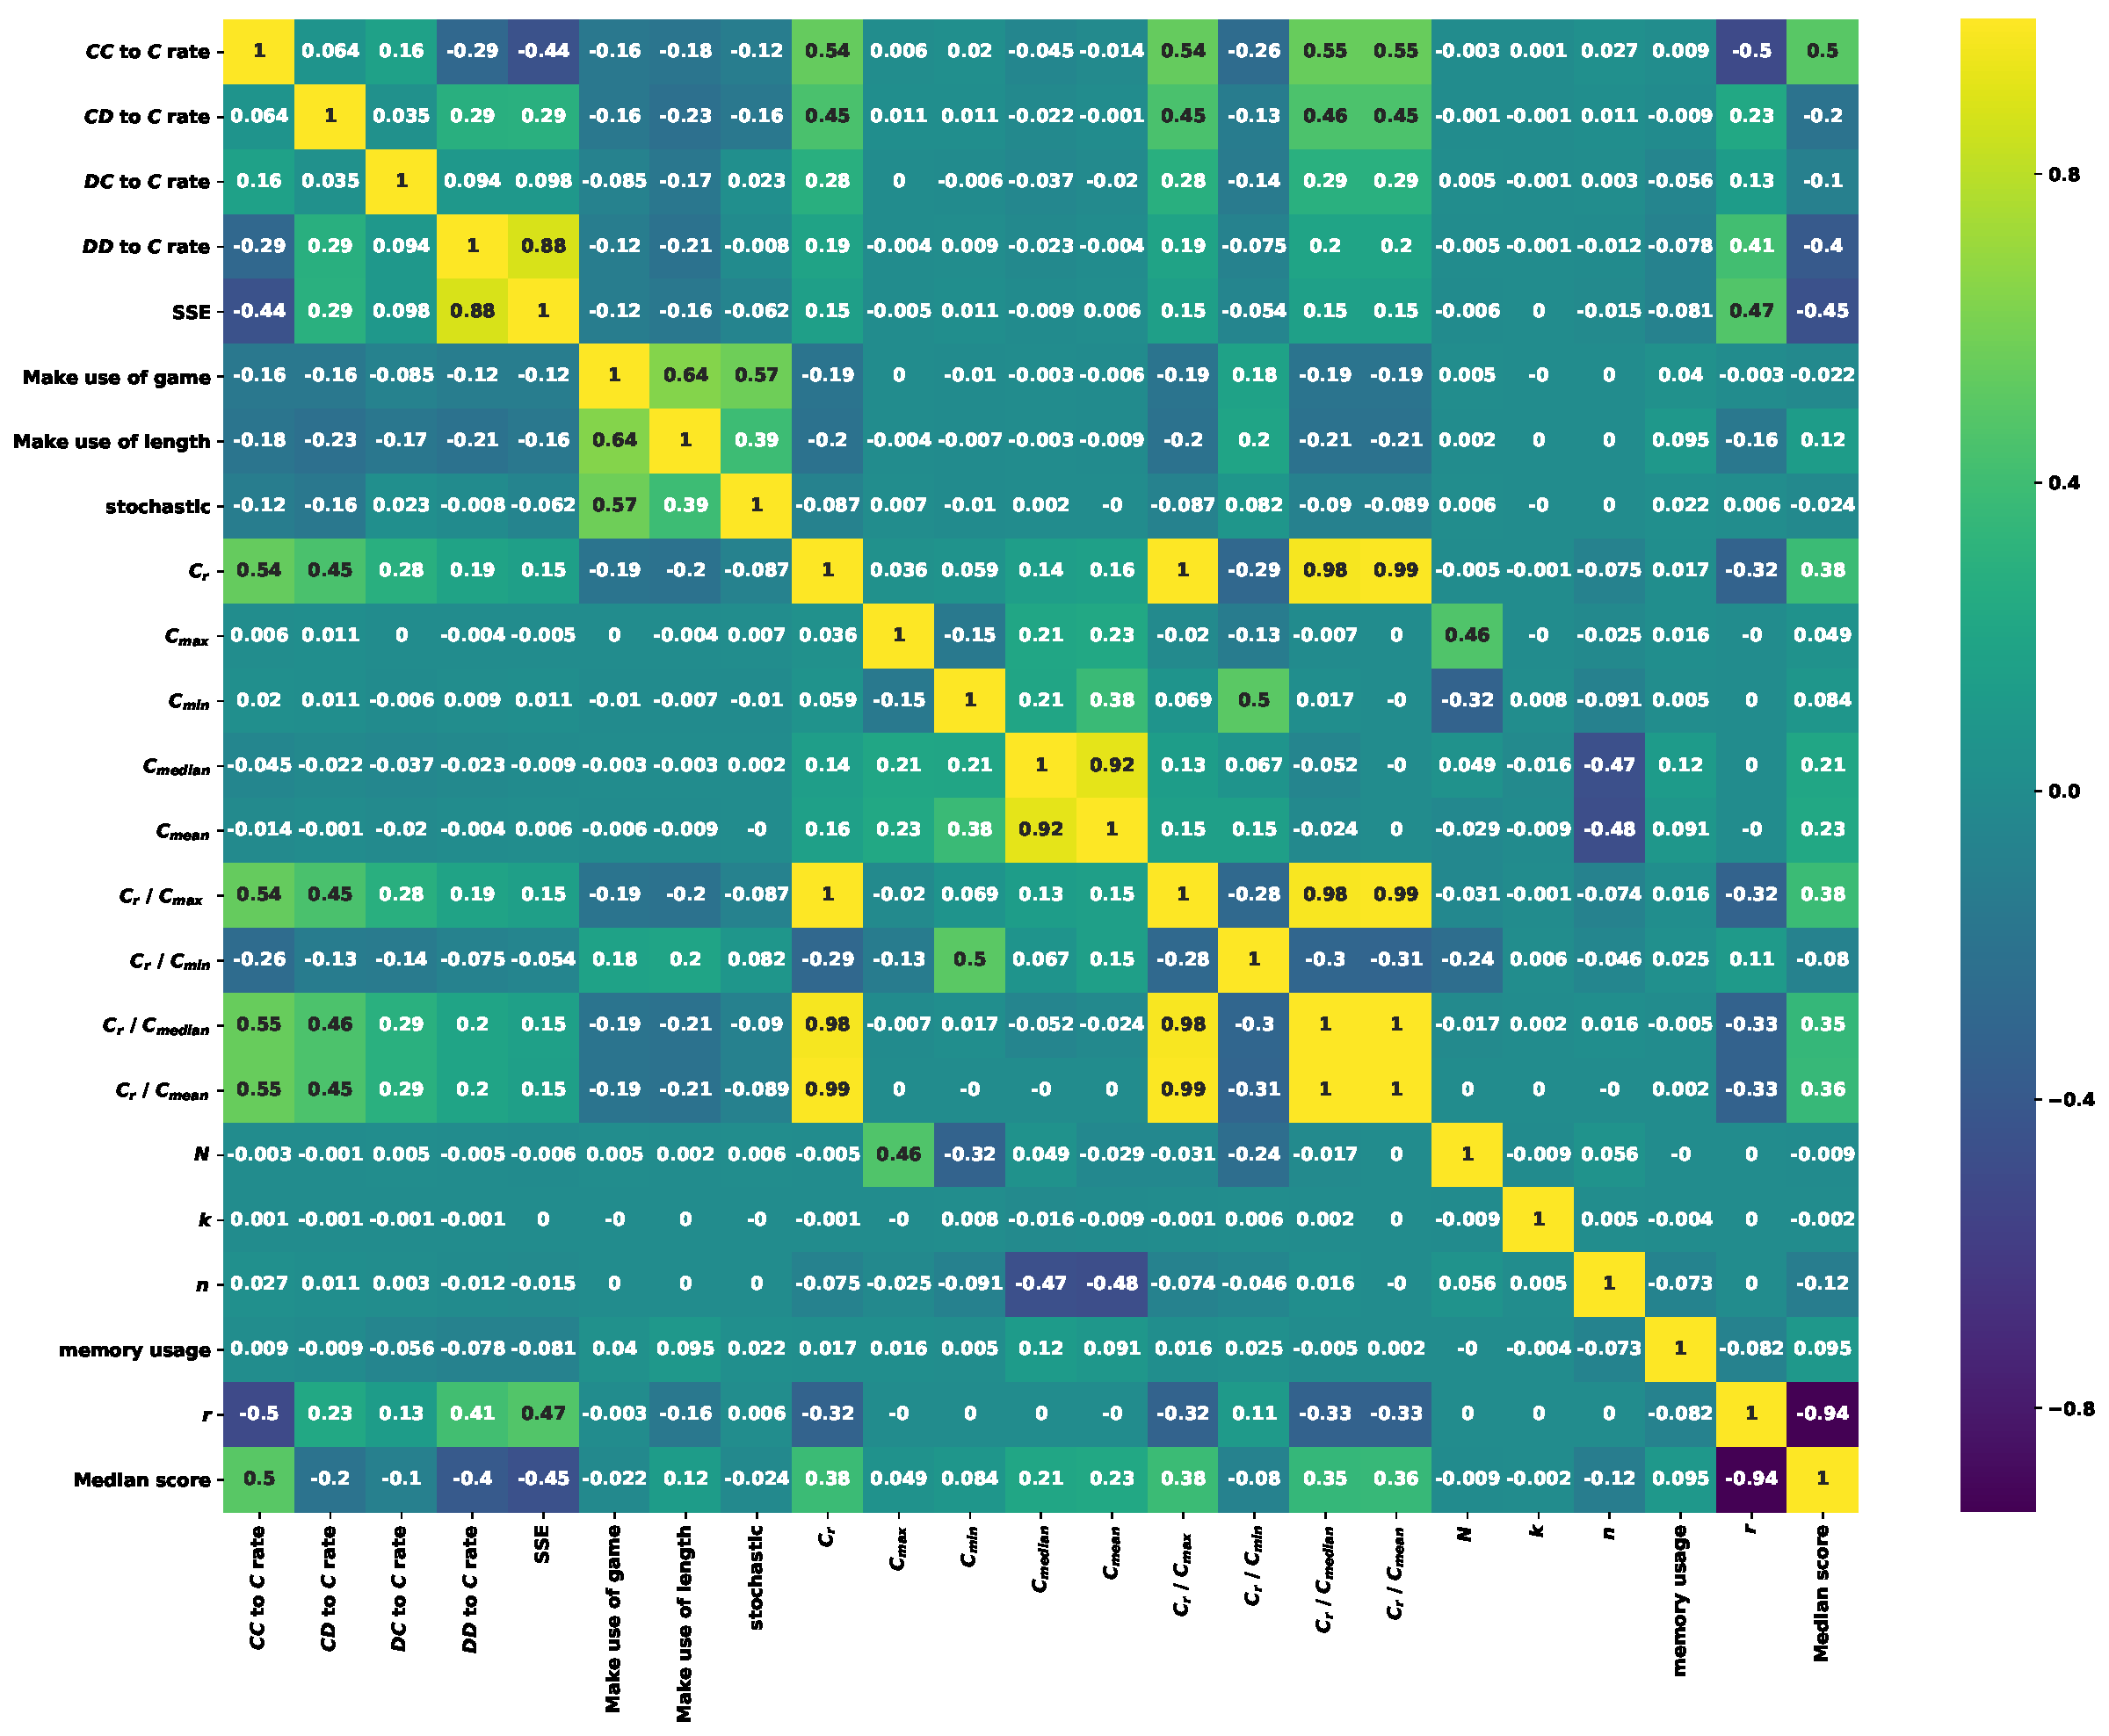
\includegraphics[width=.75\linewidth]{../images/standard_correlation_plot.pdf}
        \end{center}
        \caption{Correlation coefficients of features in Table~\ref{table:manual_features}
        for standard tournaments}
\end{figure}
\begin{figure}[!htbp]
    \begin{center}
        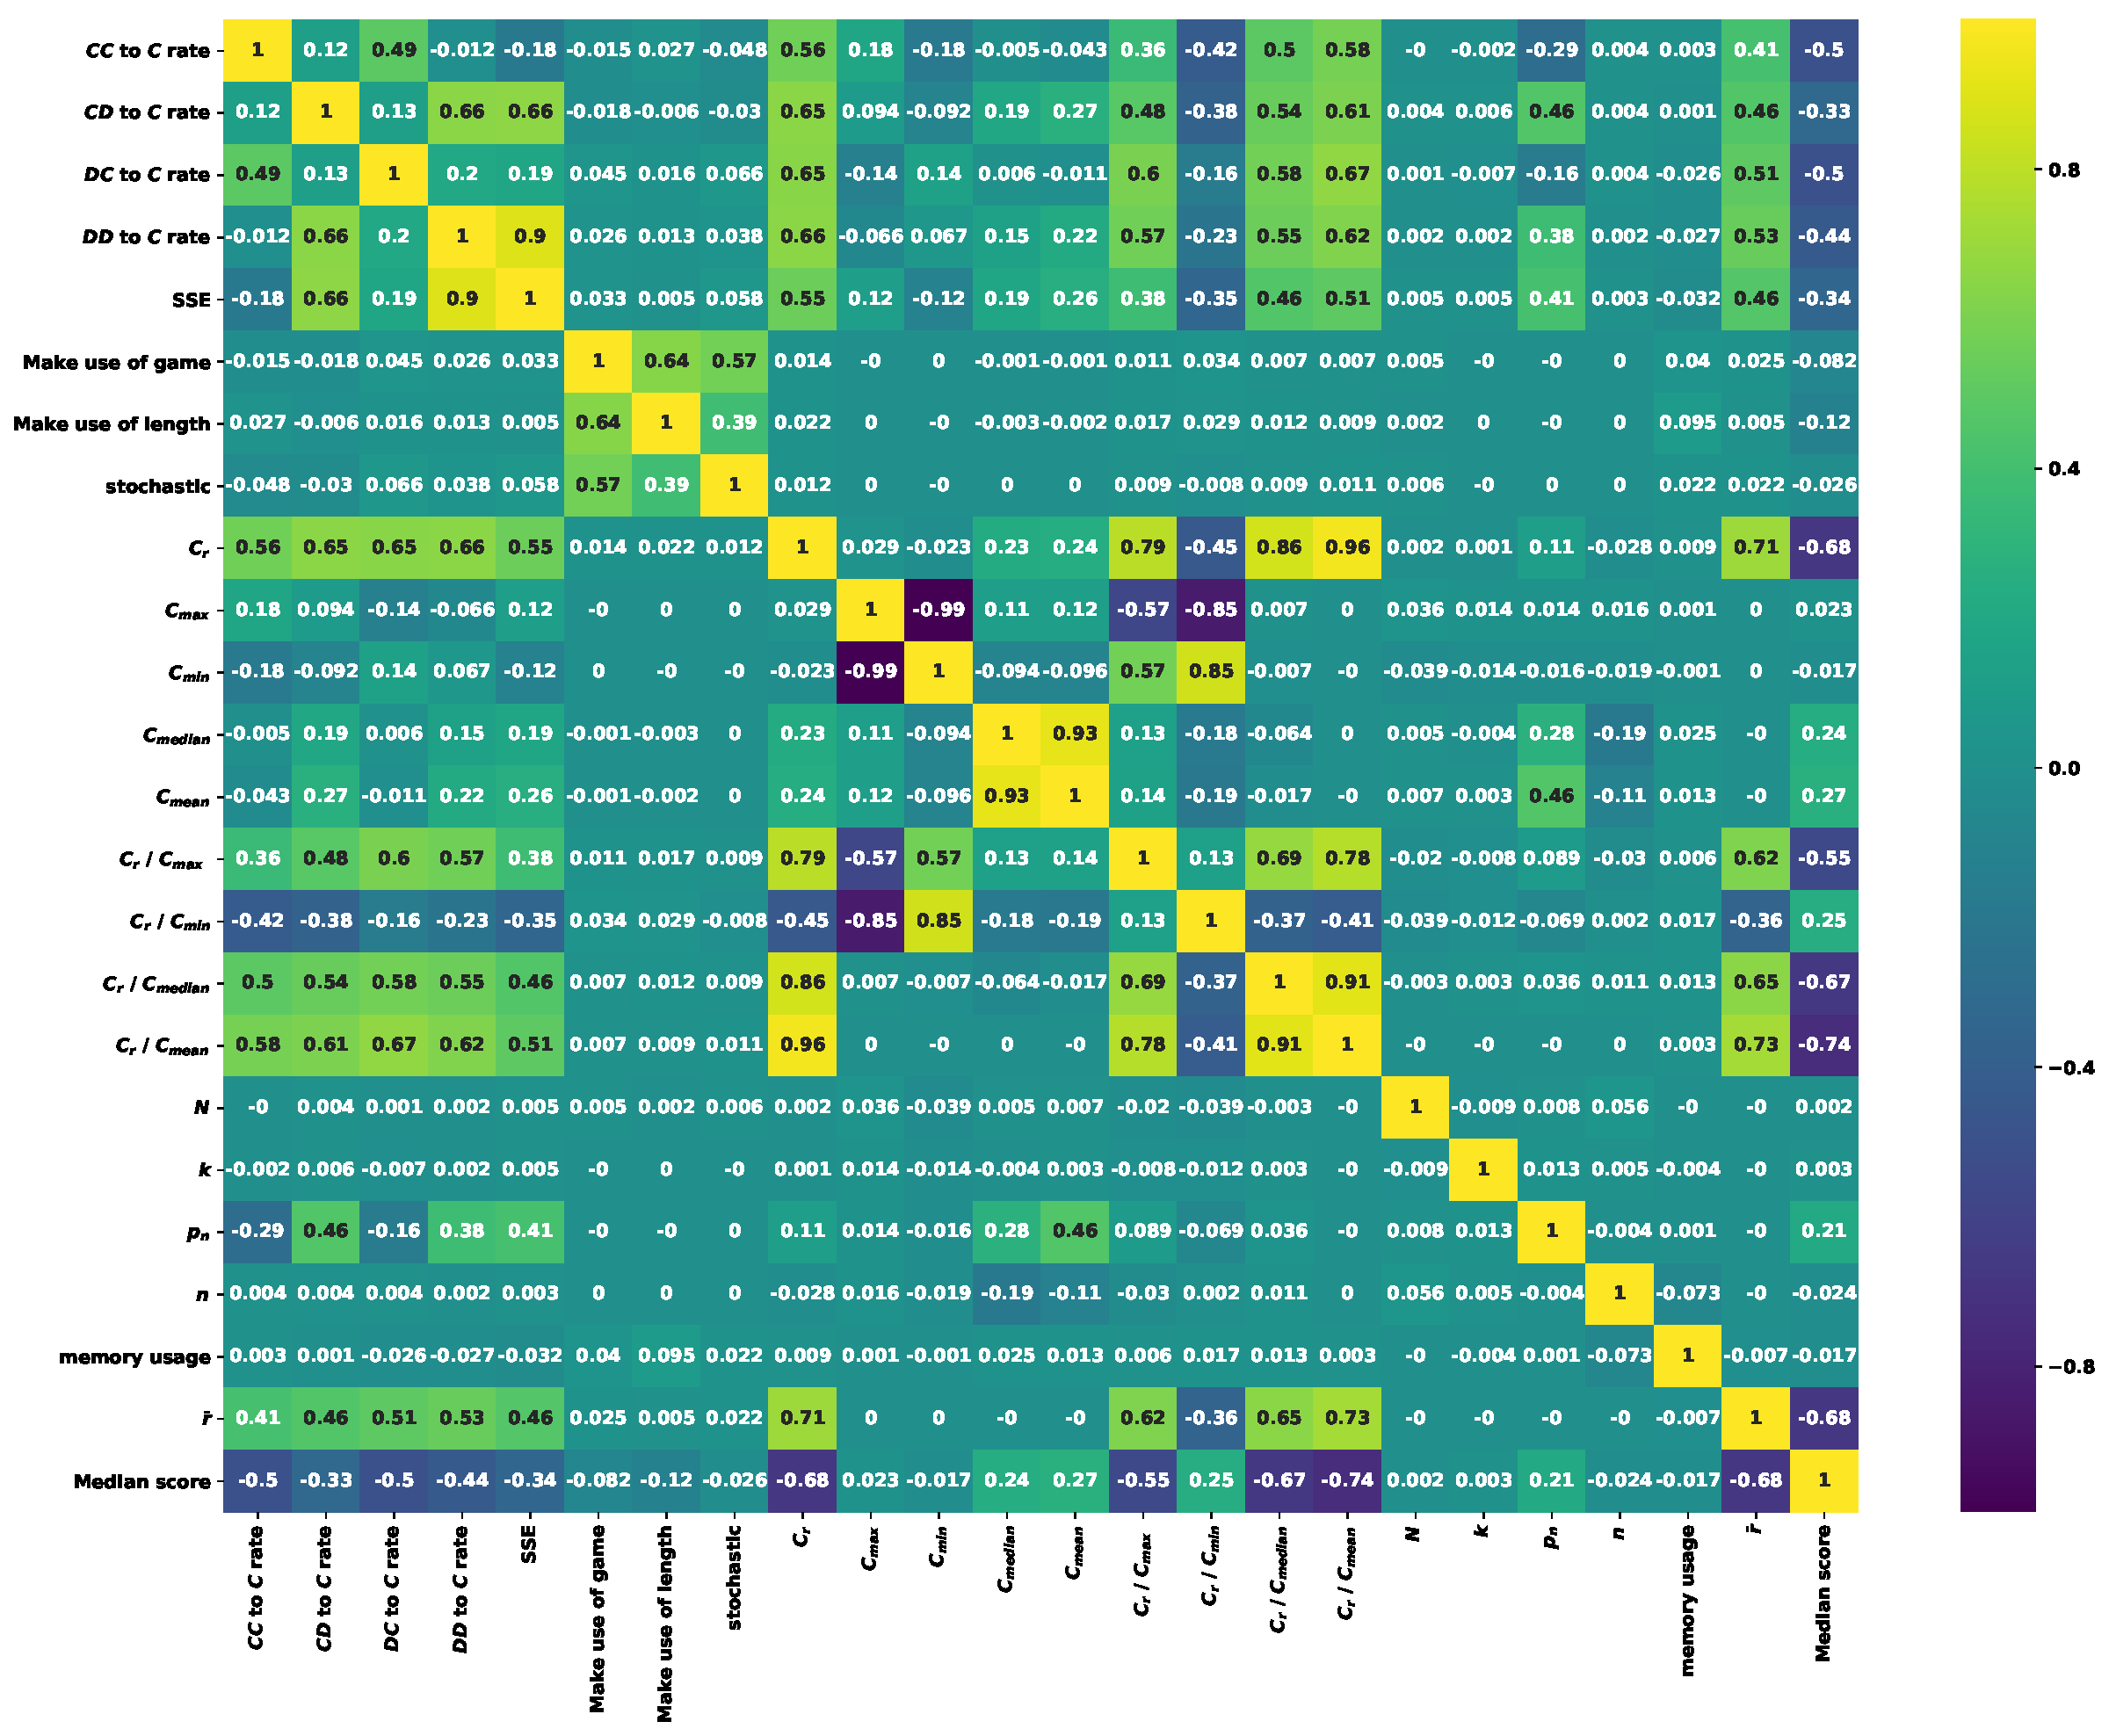
\includegraphics[width=.75\linewidth]{../images/noise_correlation_plot.pdf}
    \end{center}
    \caption{Correlation coefficients of features in Table~\ref{table:manual_features}
    for noisy tournaments}
\end{figure}
\begin{figure}[!htbp]
    \begin{center}
        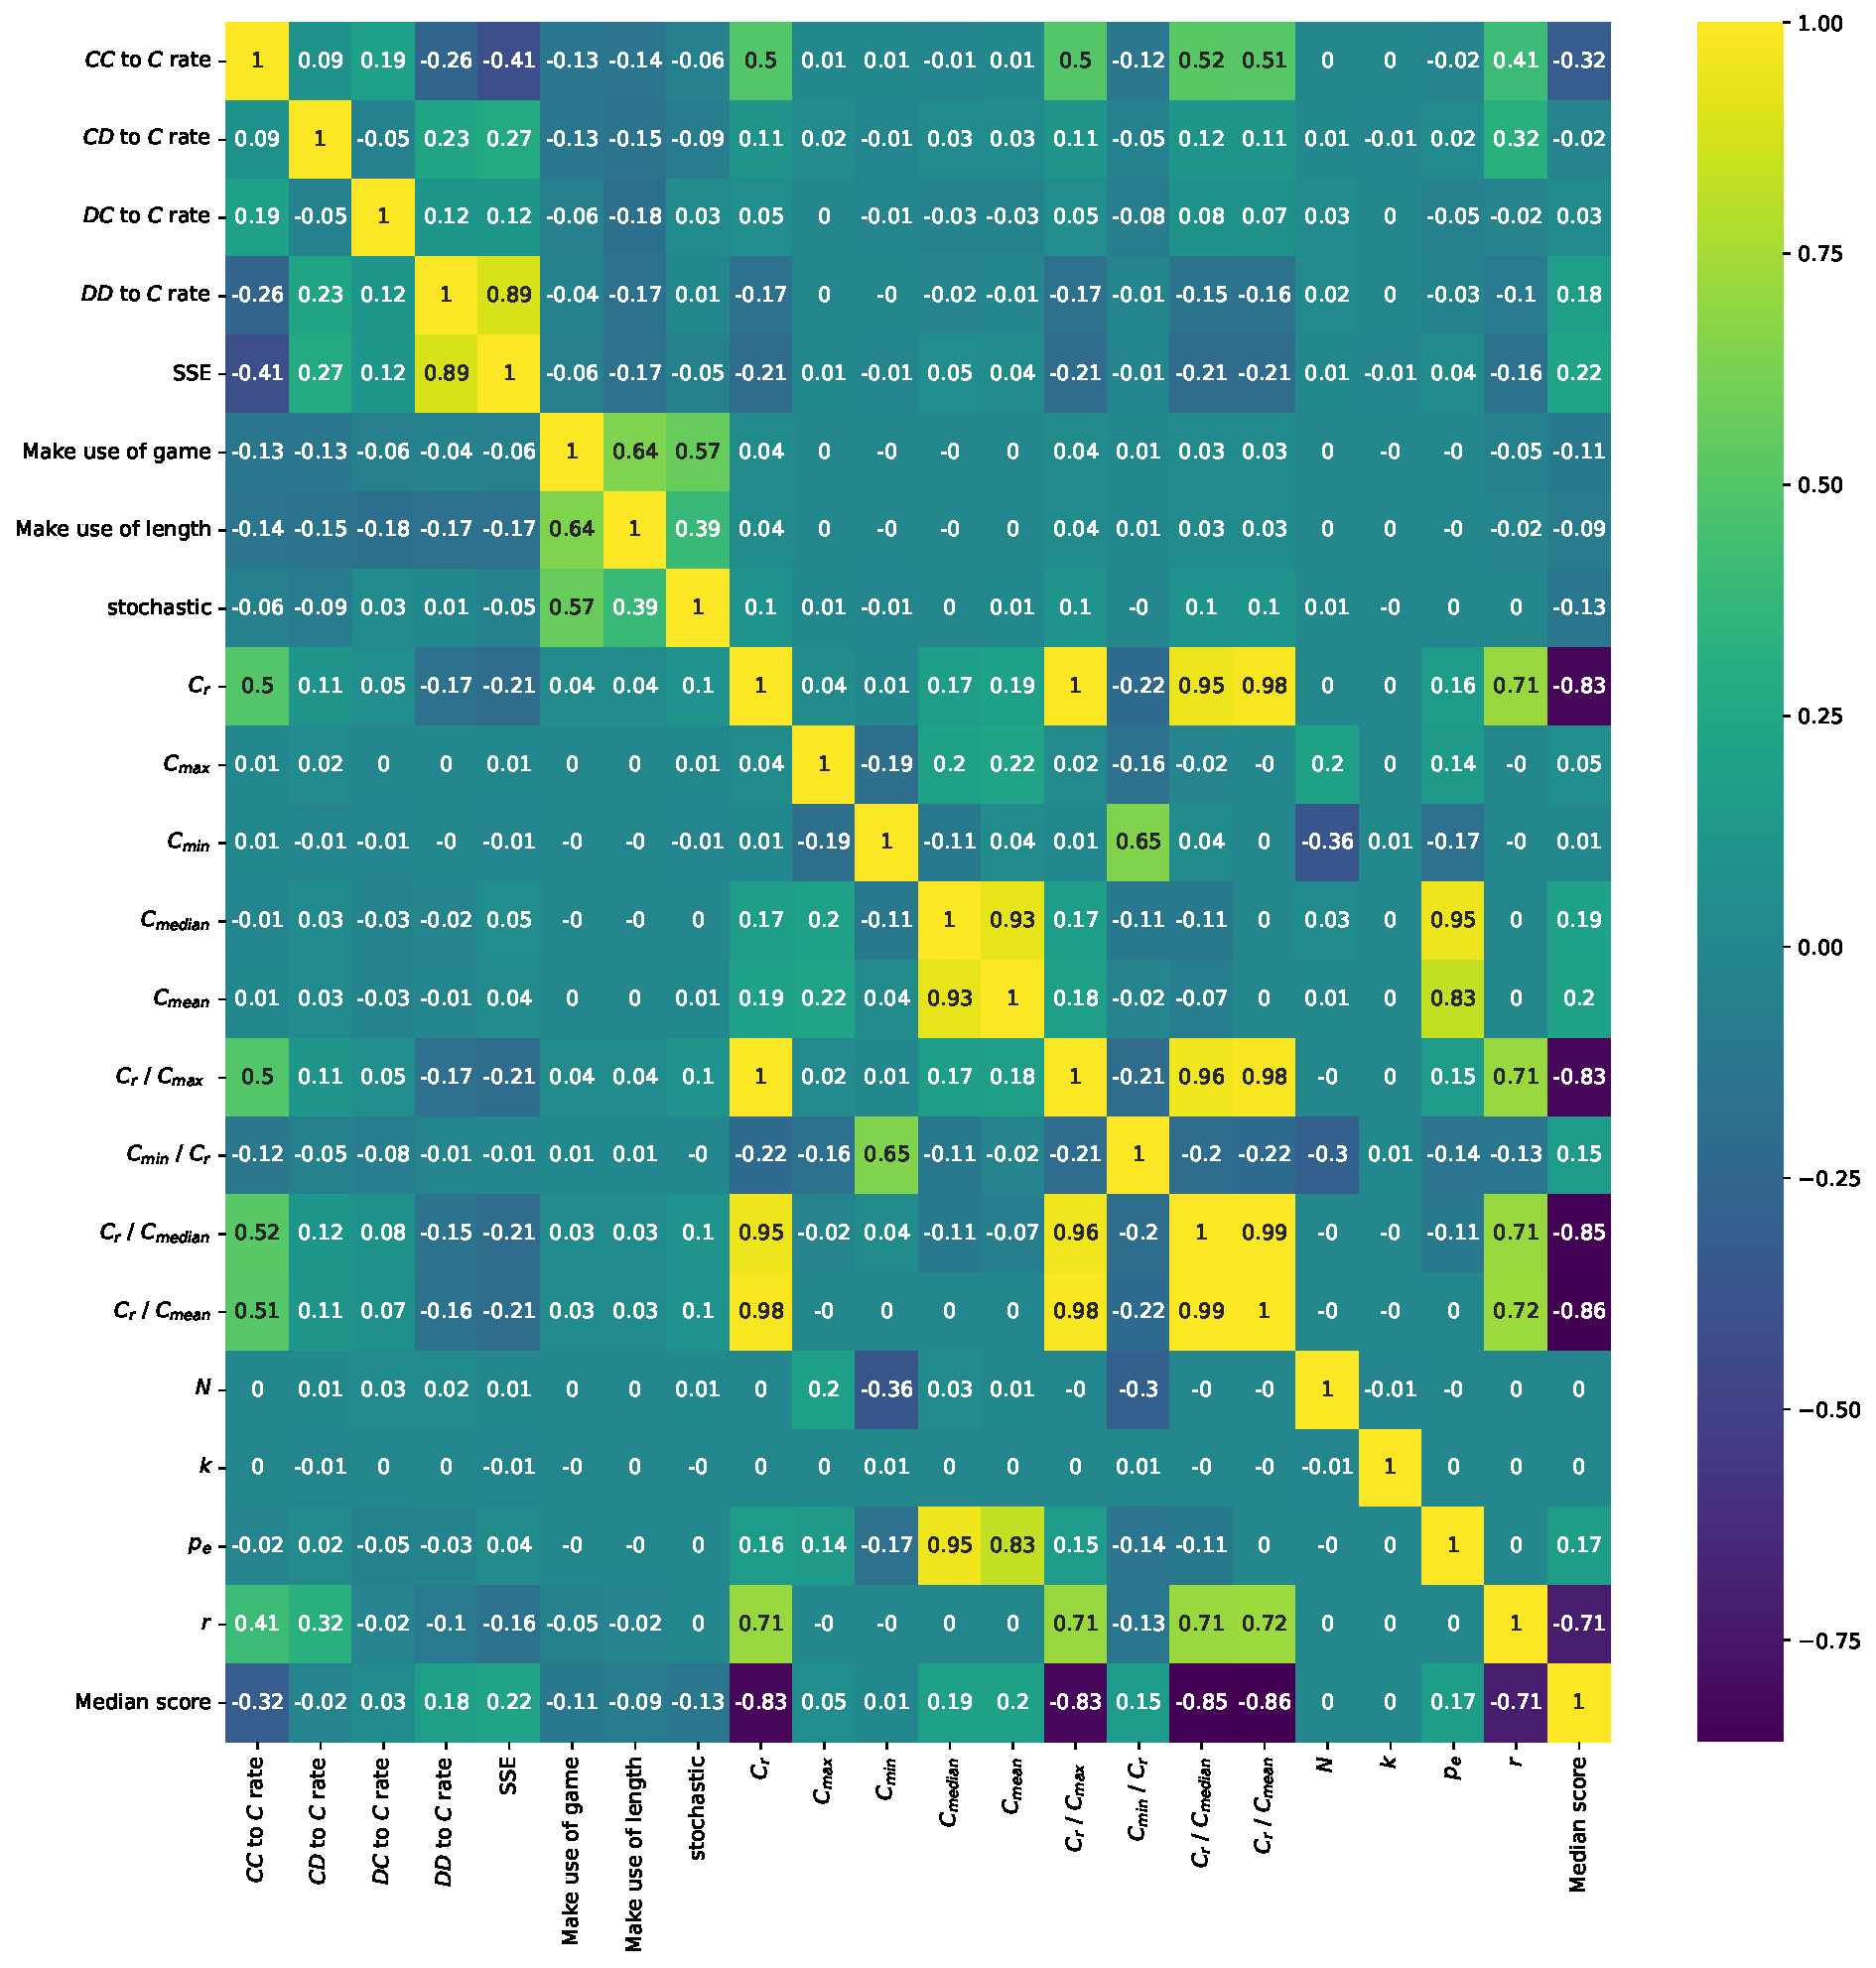
\includegraphics[width=.75\linewidth]{../images/probend_correlation_plot.pdf}
    \end{center}
    \caption{Correlation coefficients of features in Table~\ref{table:manual_features}
    for probabilistic ending tournaments}
\end{figure}
\begin{figure}[!htbp]
    \begin{center}
        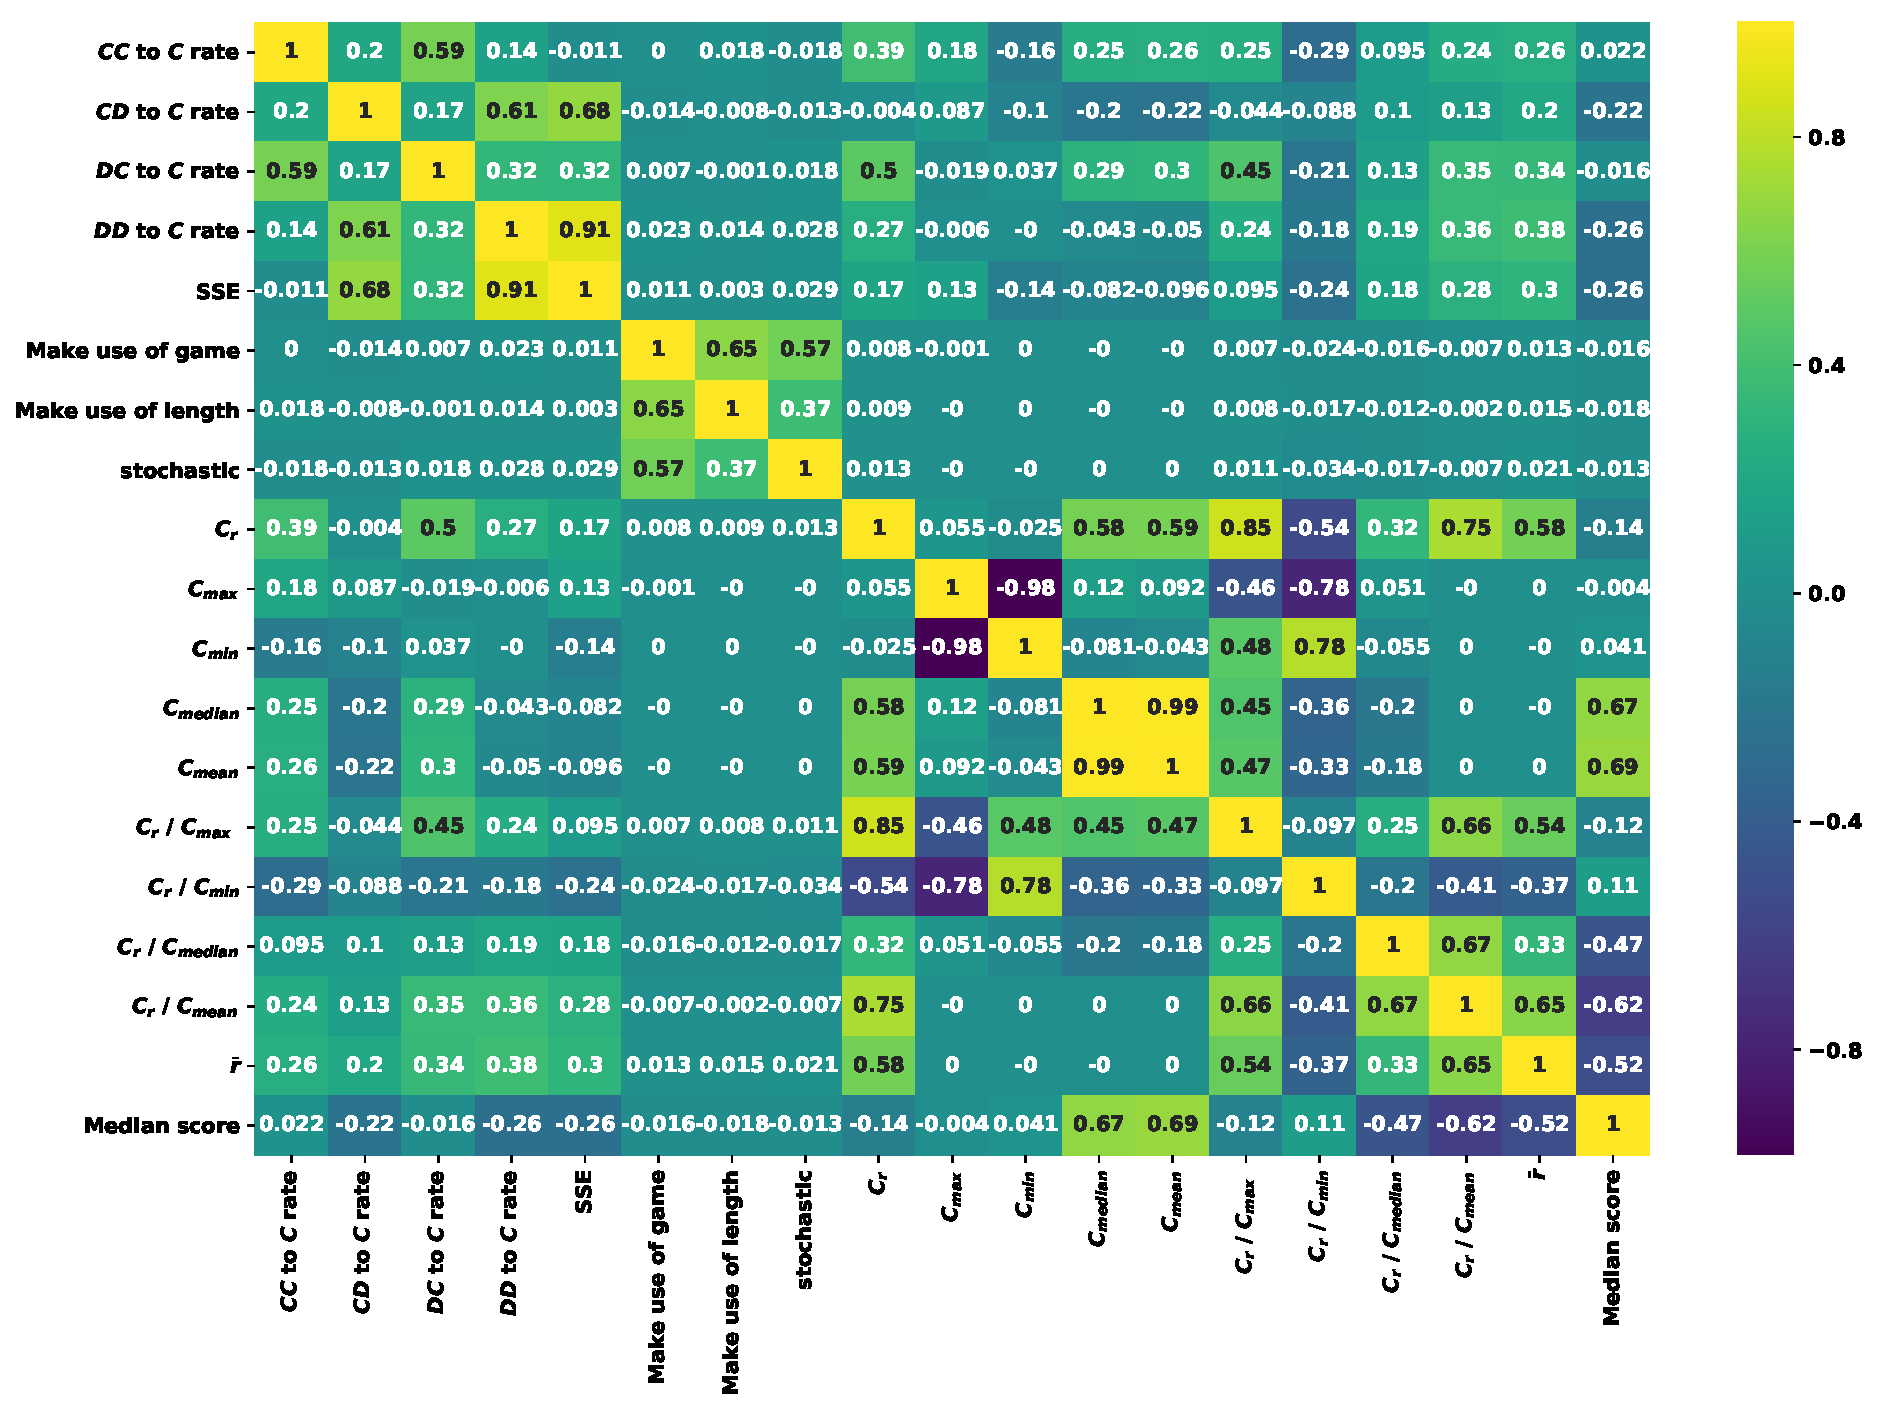
\includegraphics[width=.75\linewidth]{../images/probend_noise_correlation_plot.pdf}
    \end{center}
    \caption{Correlation coefficients of features in Table~\ref{table:manual_features}
    for noisy probabilistic ending tournaments}
\end{figure}
\begin{figure}[!htbp]
    \begin{center}
        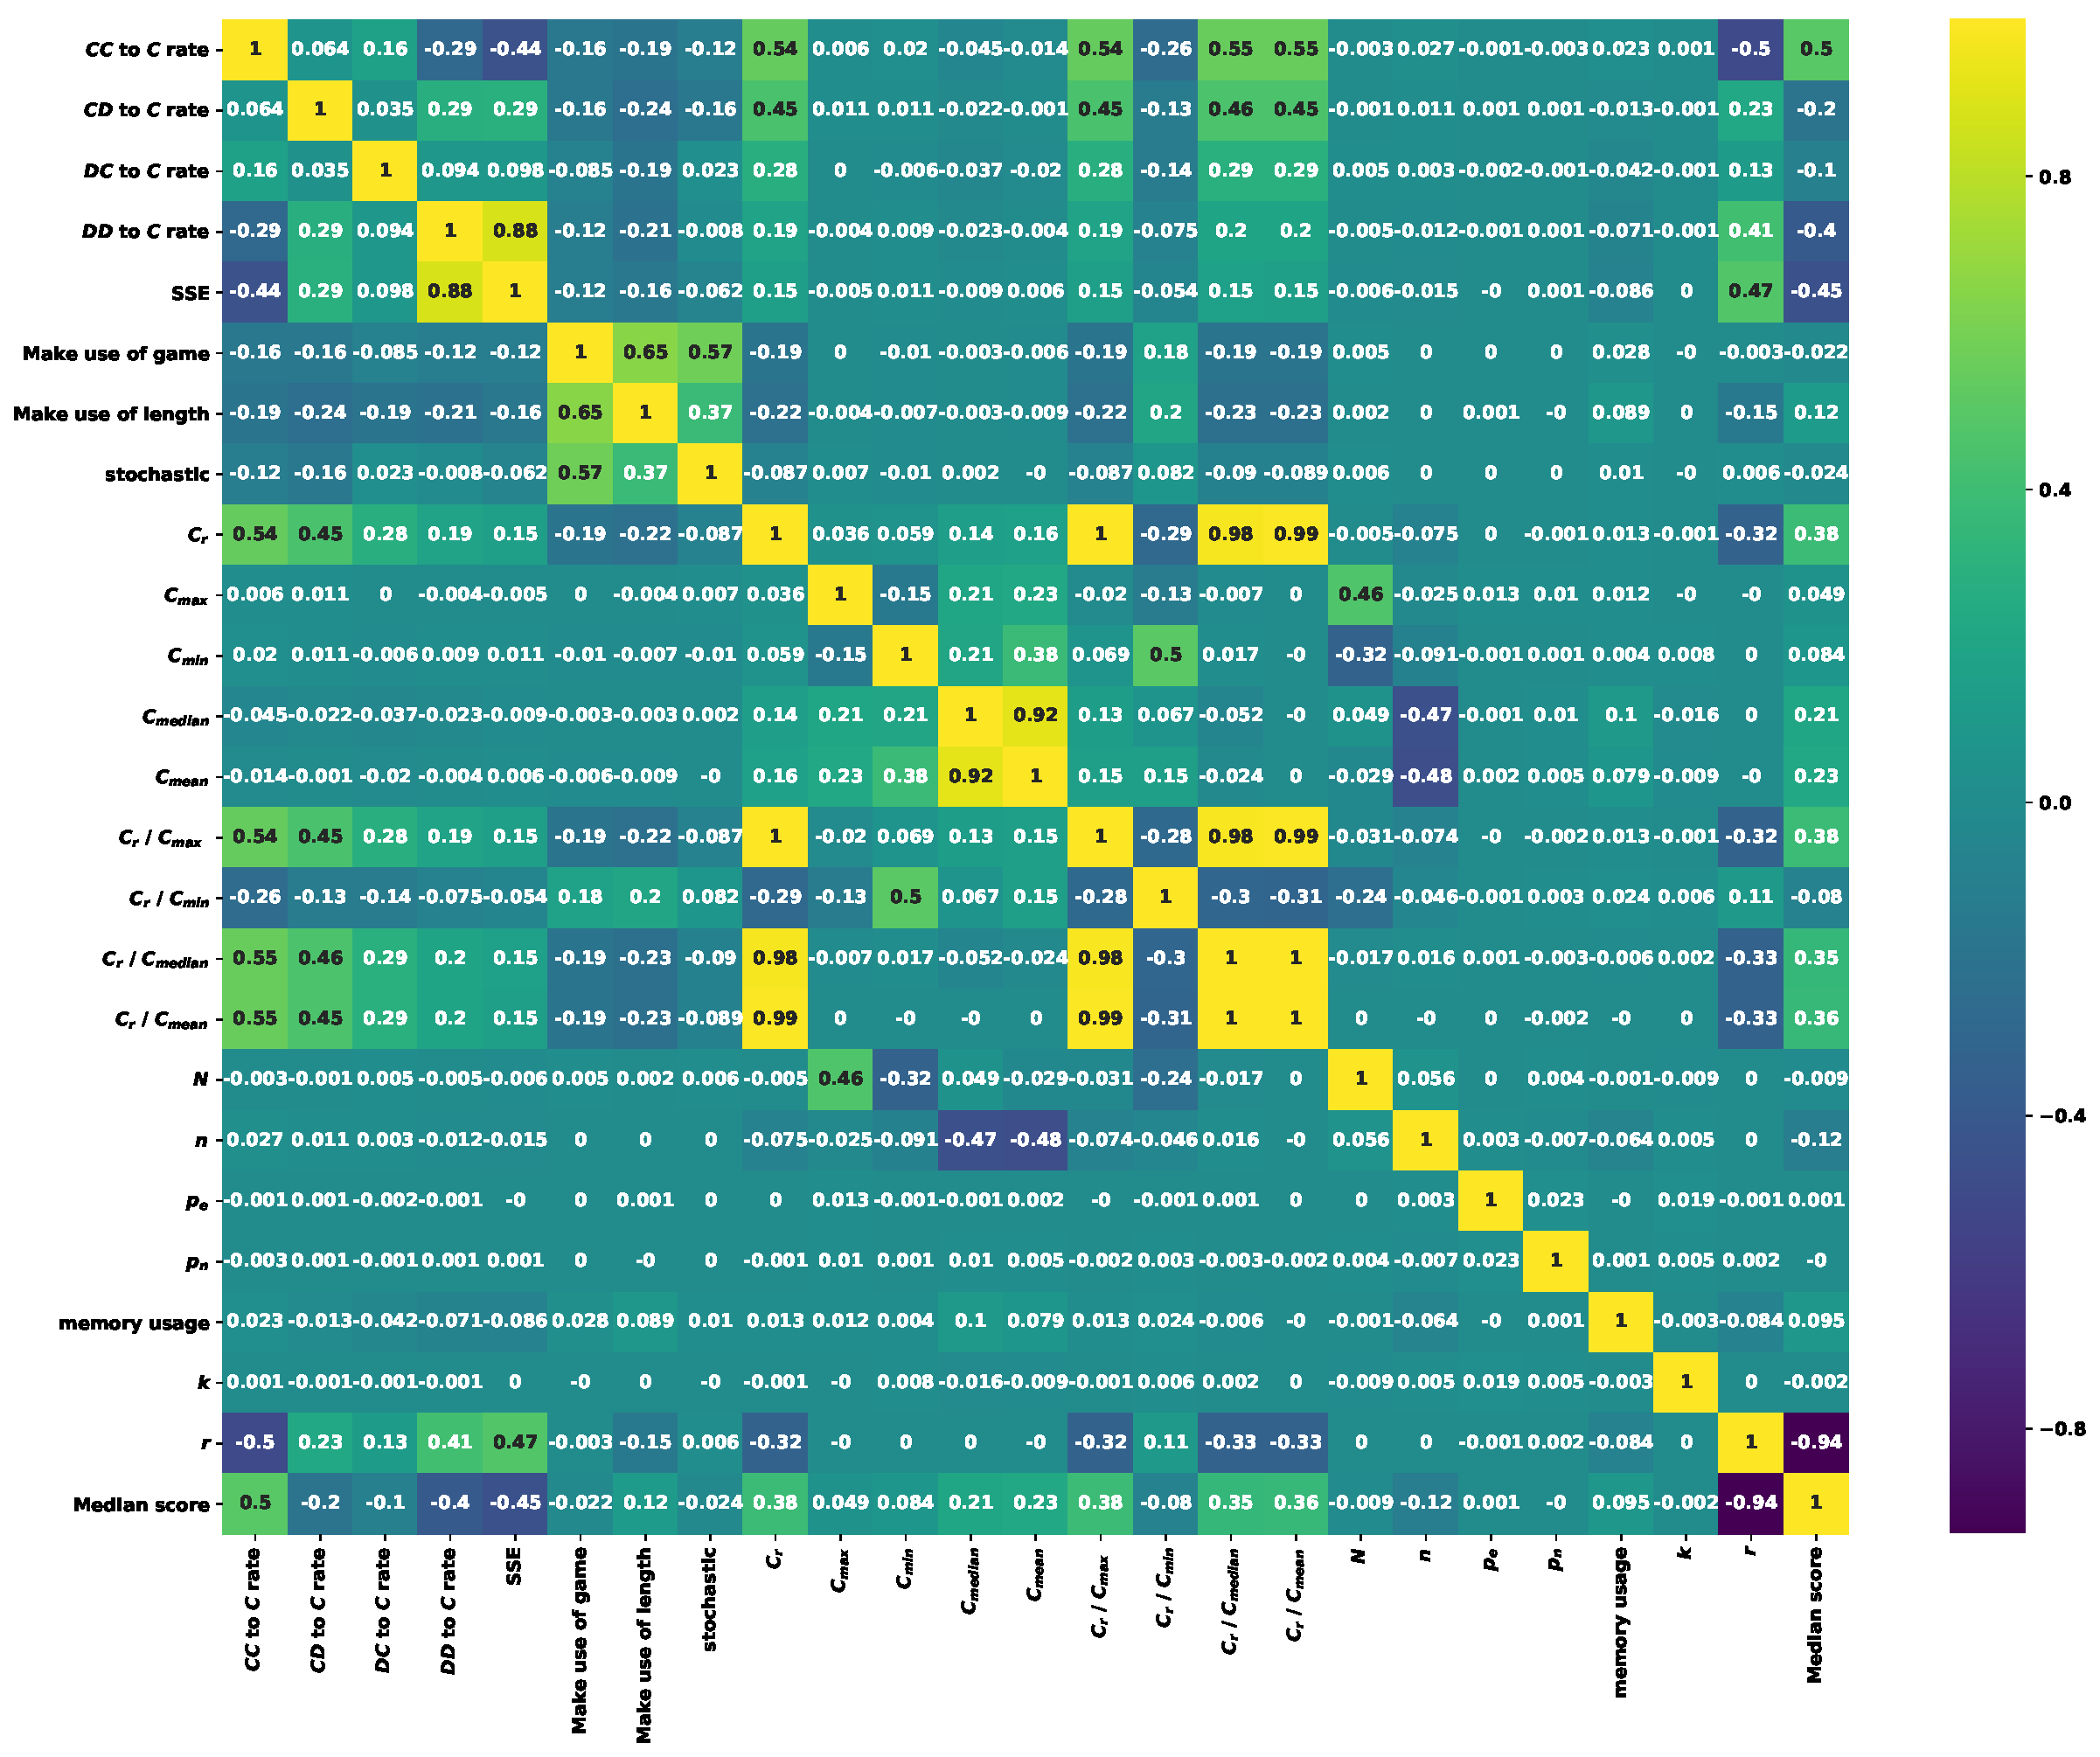
\includegraphics[width=.75\linewidth]{../images/merged_correlation_plot.pdf}
    \end{center}
    \caption{Correlation coefficients of features in Table~\ref{table:manual_features}
    for data set}
\end{figure}

\end{document}